\chapter{\igh{} locus structure and evolution in the Cyprinodontiformes}  
\label{chap:locus}
\onehalfspacing

\pagebreak

\section{Introduction}

The native structure of the immunoglobulin heavy chain (\igh{}) locus determines the state space of antibody heavy-chain diversity in a species, including the range of \vh, \dh and \jh segment choices available in VDJ recombination \parencite{jung2006vdjr}, the relationship between VDJ recombination and isotype choice \parencite{fillatreau2013astonishing}, and the ability of processes such as gene conversion \parencite{wysocki1989conversion} and class-switch recombination \parencite{magor2015affinity,patel2018aid} to affect the diversity and functionality of the antibody repertoire. The diversity produced by VDJ recombination, junctional diversity and secondary diversification processes (\Cref{sec:intro_immunity_primary,sec:intro_affinity_maturation}) in this locus are responsible for the majority of variation in antigen-specificity within a B-cell population, while the choice of isotype among the available \igh{} constant regions determines the antibody's effector function and relationship with the rest of the immune system \parencite{schroeder2010immunoglobulins}. Understanding the native structure of the \igh{} locus is therefore essential for understanding how the adaptive immune system functions in a given vertebrate species, while comparing loci between species enables the evolutionary history of adaptive immunity across lineages to be analysed, providing crucial insight into the complex history of this essential biological system. Last but not least, by providing thorough documentation of the \igh{} gene segments present in a species, characterising the \igh{} locus in a species is an essential forerunner to quantitative analysis of adaptive immunity using immunoglobulin sequencing.

Previous work has characterised \igh{} locus structure in a number of teleost species, including zebrafish \parencite{danilova2005zebrafish}, medaka \parencite{magadan2011medaka}, stickleback \parencite{bao2010stickleback,gambondeza2011stickleback}, rainbow trout \parencite{hansen2005trout}, fugu \parencite{savan2005fugu}, and Atlantic salmon \parencite{yasuike2010salmon} (\Cref{sec:intro_teleost_loci}). These characterisations have revealed remarkable diversity in the size, structure and functionality of teleost \igh{} loci. However, the number of loci characterised is very small compared to the total evolutionary diversity of teleost fish, and is mainly confined to major aquaculture species (trout, catfish, salmon) or research models (zebrafish, stickleback, medaka) \parencite{fillatreau2013astonishing,bengten2015fishantibodies}, with characterised species often quite distantly related to one another within the teleost clade. This relatively sparse sampling of teleost \igh{} loci has left wide swathes of teleost diversity without any characterised \igh{} loci, and has prevented higher-resolution analysis of locus structural evolution across closely related species.

In this chapter, therefore, I present complete characterisations of the \igh{} loci of two important model organisms from the Cyprinodontiformes, a diverse clade of primarily freshwater teleost fishes with no previously-characterised \igh{} loci. \nfu, the turquoise killifish (\Cref{sec:intro_killifish}), has recently emerged as an important model system for ageing research \parencite{harel2015platform,valenzano2015genome}, and is also of evolutionary and ecological interest due to its short lifespan, extreme natural environment, and unusual life history \parencite{cellerino2016bush}. The southern platyfish \xma, meanwhile, is an important model organism in evolutionary ecology and population genetics \parencite{schartl2013platyfish}. Comparing the \igh{} loci of these two closely-related species (\Cref{sec:nfu-locus,sec:xma-locus}) reveals dramatic and unexpected differences in immune structure, which when combined with information from previously-published loci from related species suggest unexpected patterns of locus evolution within this group of teleost fishes. Most strikingly, the specialised mucosal antibody isotype \igh{Z} appears to have been convergently lost in multiple closely-related lineages. 

To further investigate the history of \igh{Z} and other surprising features of \igh{} locus evolution in the Cyprinodontiformes, I performed a partial reconstruction and analysis of the \igh{} loci from ten further cyprinodontiform species (\Cref{fig:species-tree-large-taxa}), as well as from a new and improved genome assembly of medaka (\textit{Oryzias latipes}), with a focus on the constant-region exons present in each species (\Cref{sec:locus_comparative}). Phylogenetic analysis confirms the repeated independent loss of \igh{Z} in this lineage and provides evidence for multiple, independent \igh{Z} subclasses present ancestrally in the clade. Taken together, this analysis significantly extends our knowledge of constant-region diversity in teleost fish, and establishes the cyprinodontiforms, and especially the African killifishes, as a highly promising group of model systems for comparative evolutionary immunology.

\begin{figure}
	\centering
	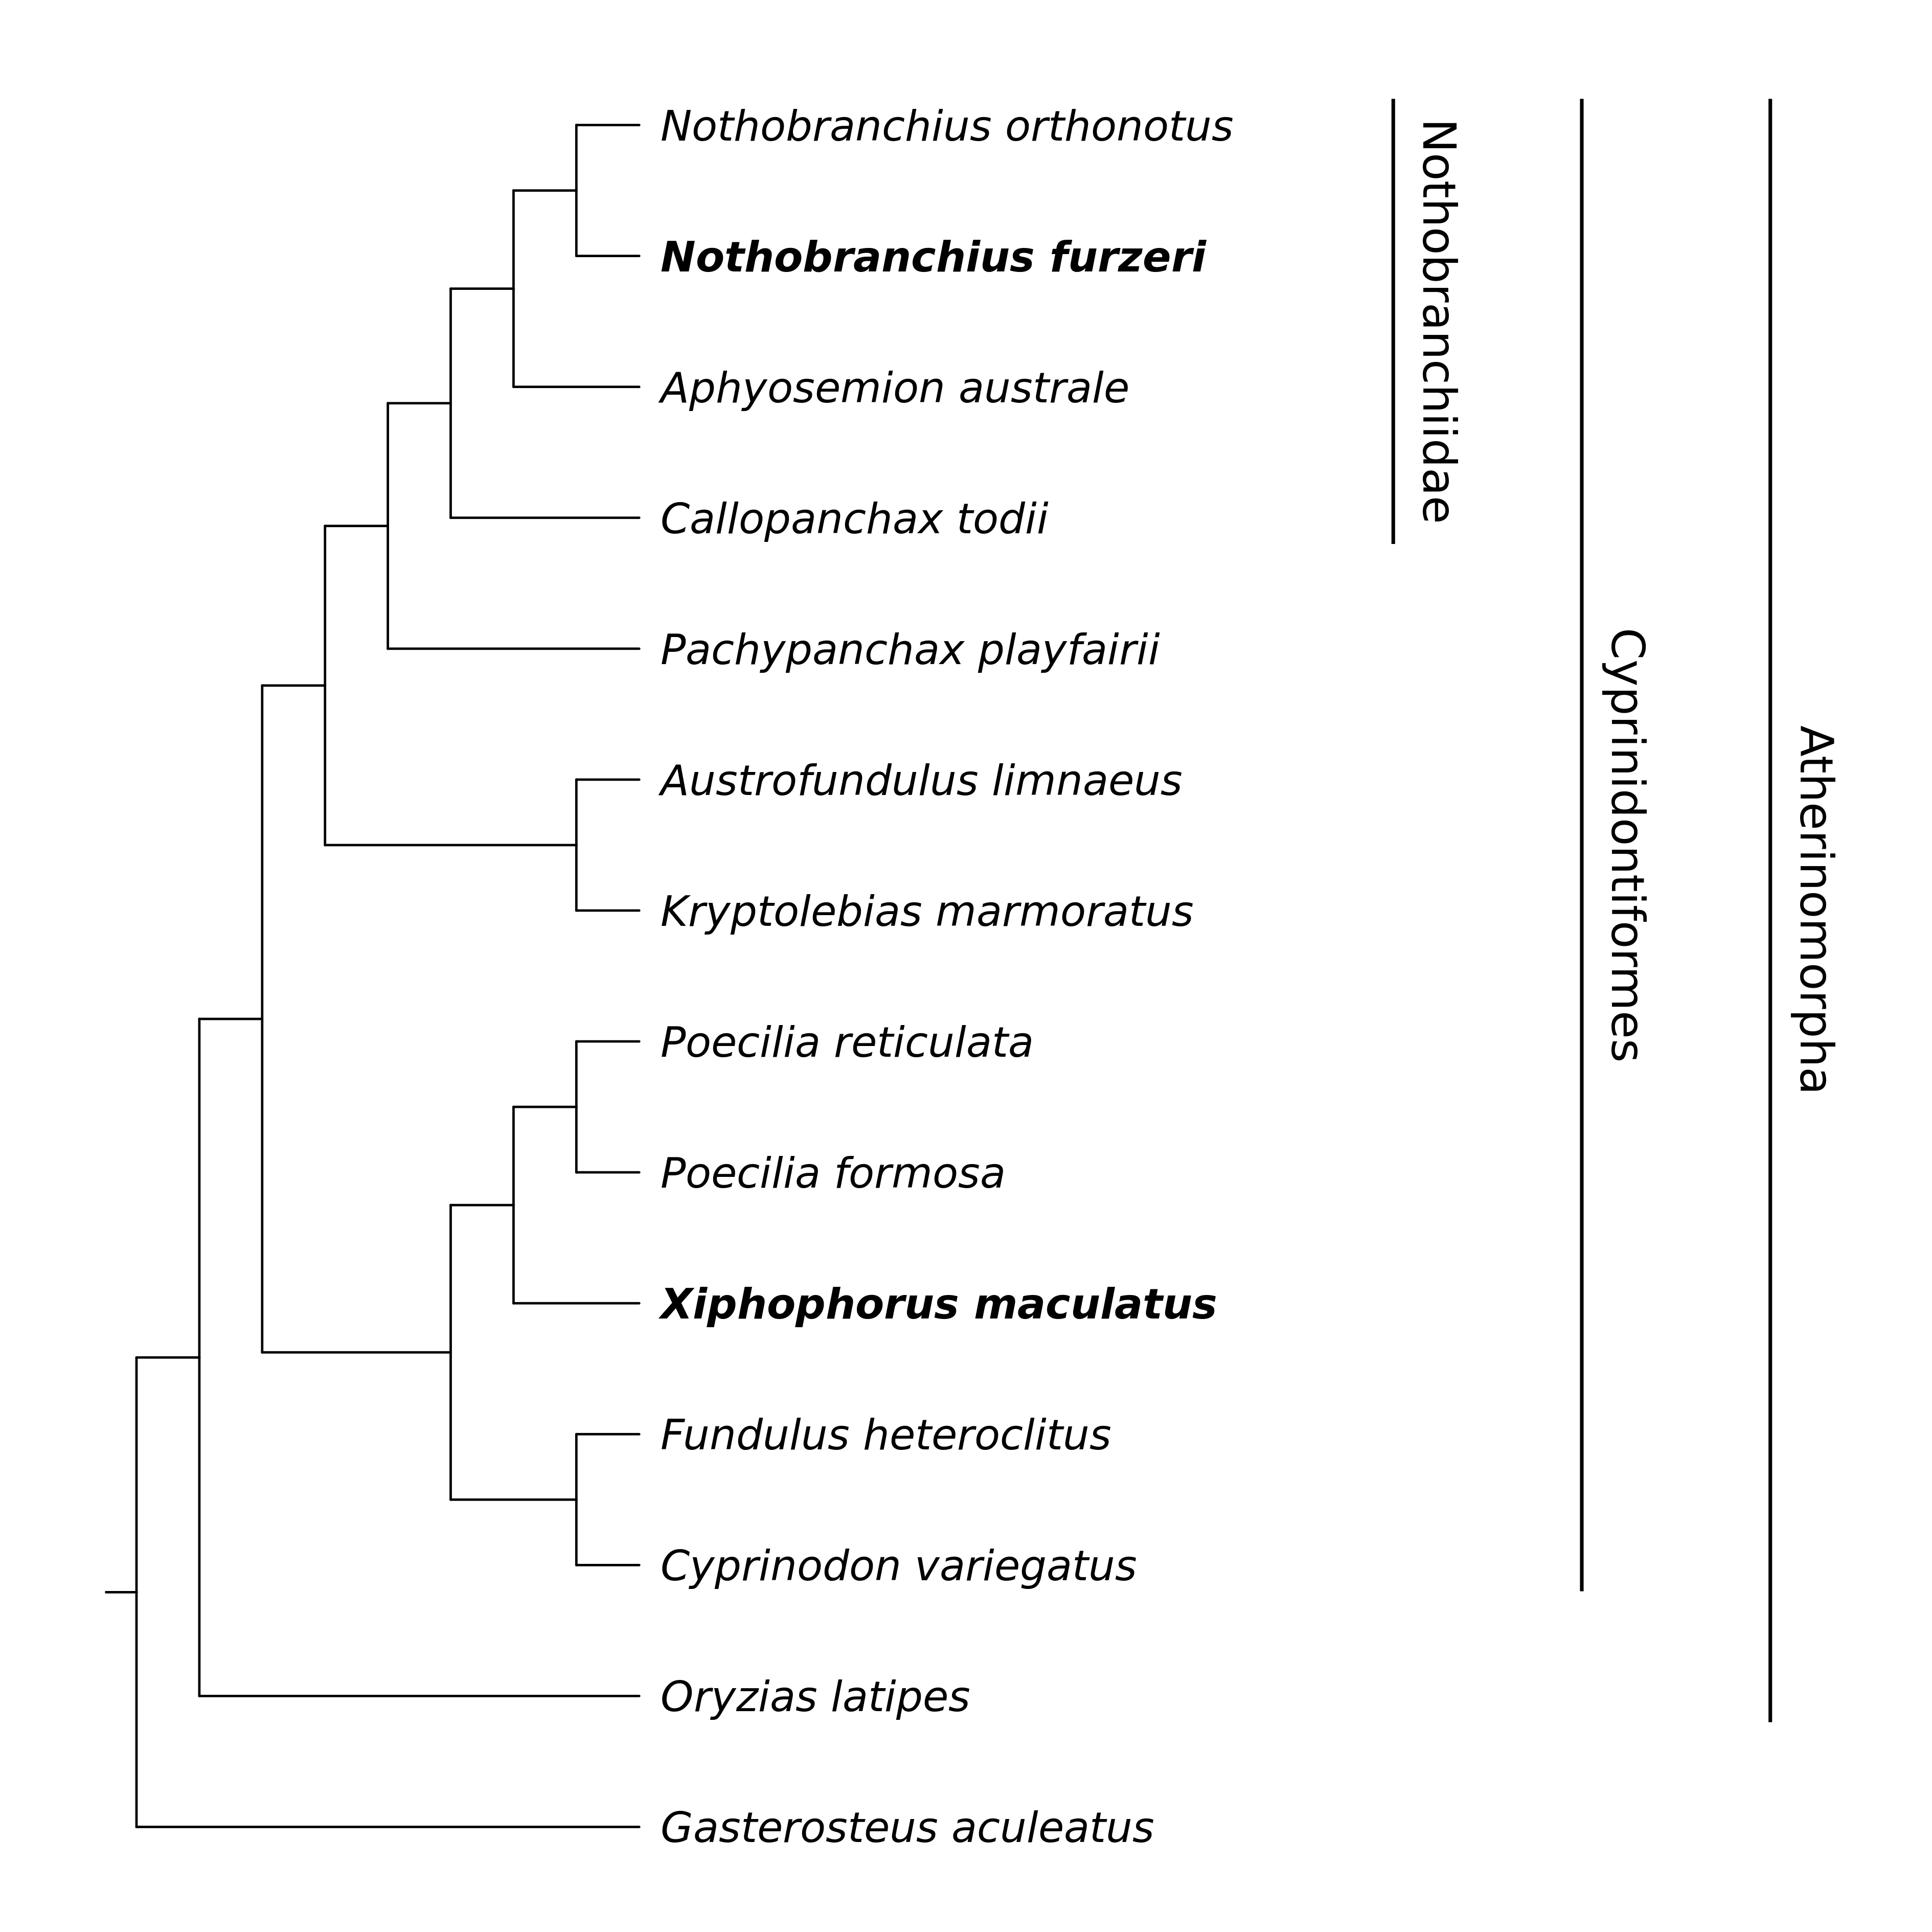
\includegraphics[width=0.9\textwidth]{_Figures/png/species-tree-large-taxa}
	\Caption{Cladogram of species included in the \igh{} locus analysis}{Boldface type indicates species for which new, complete \igh{} locus assemblies were generated for this study; other species were either previously-characterised reference species (\species{G.}{aculeatus}, \species{O.}{latipes}) or underwent constant-region characterisation only (all other species). Labelled vertical bars designate higher taxa of interest.}
	\label{fig:species-tree-large-taxa}
\end{figure}

\section{The \igh{} locus of \nfu}
\label{sec:nfu-locus}

\subsection{Assembling the \Nfu \igh{} locus}
\label{sec:nfu-locus-assembly}

In order to locate and characterise the \nfu \igh{} locus, I collated databases of \vh, \jh, and \ch exon sequences from the published locus sequences of three reference species (zebrafish \parencite{danilova2005zebrafish}, three-spined stickleback \parencite{bao2010stickleback,gambondeza2011stickleback}, and medaka \parencite{magadan2011medaka}, \Cref{sec:methods_comp_locus_reference}) and aligned them to the \nfu genome (NFZ V2.0 \parencite{willemsen2019popgen}) with \program{BLAST} \parencite{altschul1990blast,altschul1997blast}. Genome scaffolds with high-confidence alignments to at least two distinct segment types or covering at least 1\,\% of the scaffold's total length were retained for downstream analysis as potential locus candidates (\Cref{sec:methods_comp_locus_scaffolds}); in total, one chromosome (chr6) and 6 unincorporated scaffolds were identified in this way (\Cref{tab:nfu-locus-scaffolds}), with chromosome 6 bearing the majority of identified gene segments.

\begin{table}[bh]
\centering
\caption{\Nfu genome scaffolds containing putative \igh{} locus fragments}
\begin{threeparttable}
\begin{tabular}{cccccccc}\toprule
\textbf{Scaffold} & \textbf{Total length (kb)} & \textbf{V} & \textbf{J} & \textbf{\cm{}} & \textbf{\cd{}} & \textbf{\cz{}} & Included in locus?\\\midrule
chr6 & 6195.6 & 15 & 7 & 5 & 11 & 0 & Yes\\\midrule
scf10901 & 1.4 & 0 & 0 & 0 & 3 & 0 & Yes\\
scf21863 & 13.5 & 1 & 0 & 0 & 0 & 0 & No\\
scf35954 & 16.3 & 3 & 0 & 0 & 0 & 0 & No\\
scf36277 & 18.9 & 2 & 1 & 0 & 0 & 0 & No\\
scf37083 & 17.7 & 1 & 0 & 0 & 0 & 0 & No\\
scf9157 & 7.2 & 0 & 7 & 4 & 0 & 0 & Yes\\\bottomrule
\end{tabular}

\end{threeparttable}
\label{tab:nfu-locus-scaffolds}
\end{table}

\begin{table}[bh]
\centering
\caption{\Nfu BAC-library inserts containing putative \igh{} locus fragments}
\begin{threeparttable}
\begin{tabular}{cccccccc}\toprule
\textbf{BAC ID} & \textbf{Insert length (kb)} & \textbf{V} & \textbf{J} & \textbf{\cm{}} & \textbf{\cd{}} & \textbf{\cz{}} & Included in locus?\\\midrule
154G24 & 106.6 & 17 & 1 & 0 & 0  & 0 & No\\
162F04 & 119.4 & 5  & 1 & 0 & 0  & 0 & No\\
165M01 & 110.7 & 15 & 1 & 0 & 0  & 0 & Yes\\
206K13 & 106.7 & 17 & 1 & 0 & 0  & 0 & No\\
208A08 & 103.2 & 17 & 1 & 0 & 0  & 0 & Yes\\
209K12 & 133.0 & 1  & 8 & 4 & 20 & 0 & Yes\\
220O06 & 104.8 & 4  & 1 & 0 & 0  & 0 & No\\
223M21 & 99.3  & 17 & 1 & 0 & 0  & 0 & No\\
248A22 & 47.3  & 7  & 0 & 0 & 0  & 0 & No\\
276N03 & 127.9 & 7  & 0 & 0 & 0  & 0 & Yes\\
277J10 & 120.8 & 17 & 1 & 0 & 0  & 0 & Yes\\
\bottomrule\end{tabular}

\end{threeparttable}
\label{tab:nfu-locus-bacs}
\end{table}

In order to determine which of the putative locus scaffolds were in fact part of the \igh{} locus, integrate these into a contiguous locus sequence, and provide additional information on any missing gene segments, I supplemented the locus assembly with insert sequences from bacterial artificial chromosomes in the turquoise-killifish genomic BAC library \parencite{reichwald2015genome}. BAC candidates (whose ends had already been sequenced as part of the genome project) were identified as potentially containing part of the locus sequence (\Cref{sec:methods_comp_bacs_ident}) on the basis of their ends aligning to promising candidate scaffolds from a previous genome assembly (first round) or to the insert sequences of previously sequenced BAC inserts (second round). Once identified,  BAC candidates were isolated from culture by alkaline lysis (\Cref{sec:methods_molec_bacs}), sequenced on an Illumina MiSeq sequencing machine, and assembled and scaffolded with \program{SPAdes} and \program{SSPACE}, respectively (\Cref{sec:methods_comp_bacs_trim,sec:methods_comp_bacs_assembly}). Complete BAC insert assemblies were generated from these scaffolds by manual alignment to overlapping genome scaffolds and other BAC inserts, combined with PCR and Sanger sequencing of intervening sequences.

Having obtained complete insert sequences for promising BAC candidates, I screened them for \igh{} locus segments in the same manner described for genome scaffolds. Passing insert sequences (\Cref{tab:nfu-locus-bacs}) were aligned to and integrated with the identified candidate scaffolds to produce a contiguous locus assembly (\Cref{sec:methods_comp_locus_final}). To minimise the probability of losing relevant gene segments to assembly errors, I gave priority in the event of a sequence conflict between BACs and scaffolds first to any sequence containing a segment missing from the other; if neither the BAC assembly nor the genome scaffolds met this condition, I prioritised the genome scaffold over the BAC assembly. In total, 3 candidate scaffolds (including chromosome 6) and 5 BAC inserts were included in the final locus assembly, while 4 scaffolds and 6 BACs were excluded as likely representing isolated \igh{} orphon segments elsewhere in the genome. The regions of the final locus sequence contributed by different BACs and scaffolds are shown in \Cref{fig:nfu-locus-aln}.

\begin{figure}
\centering
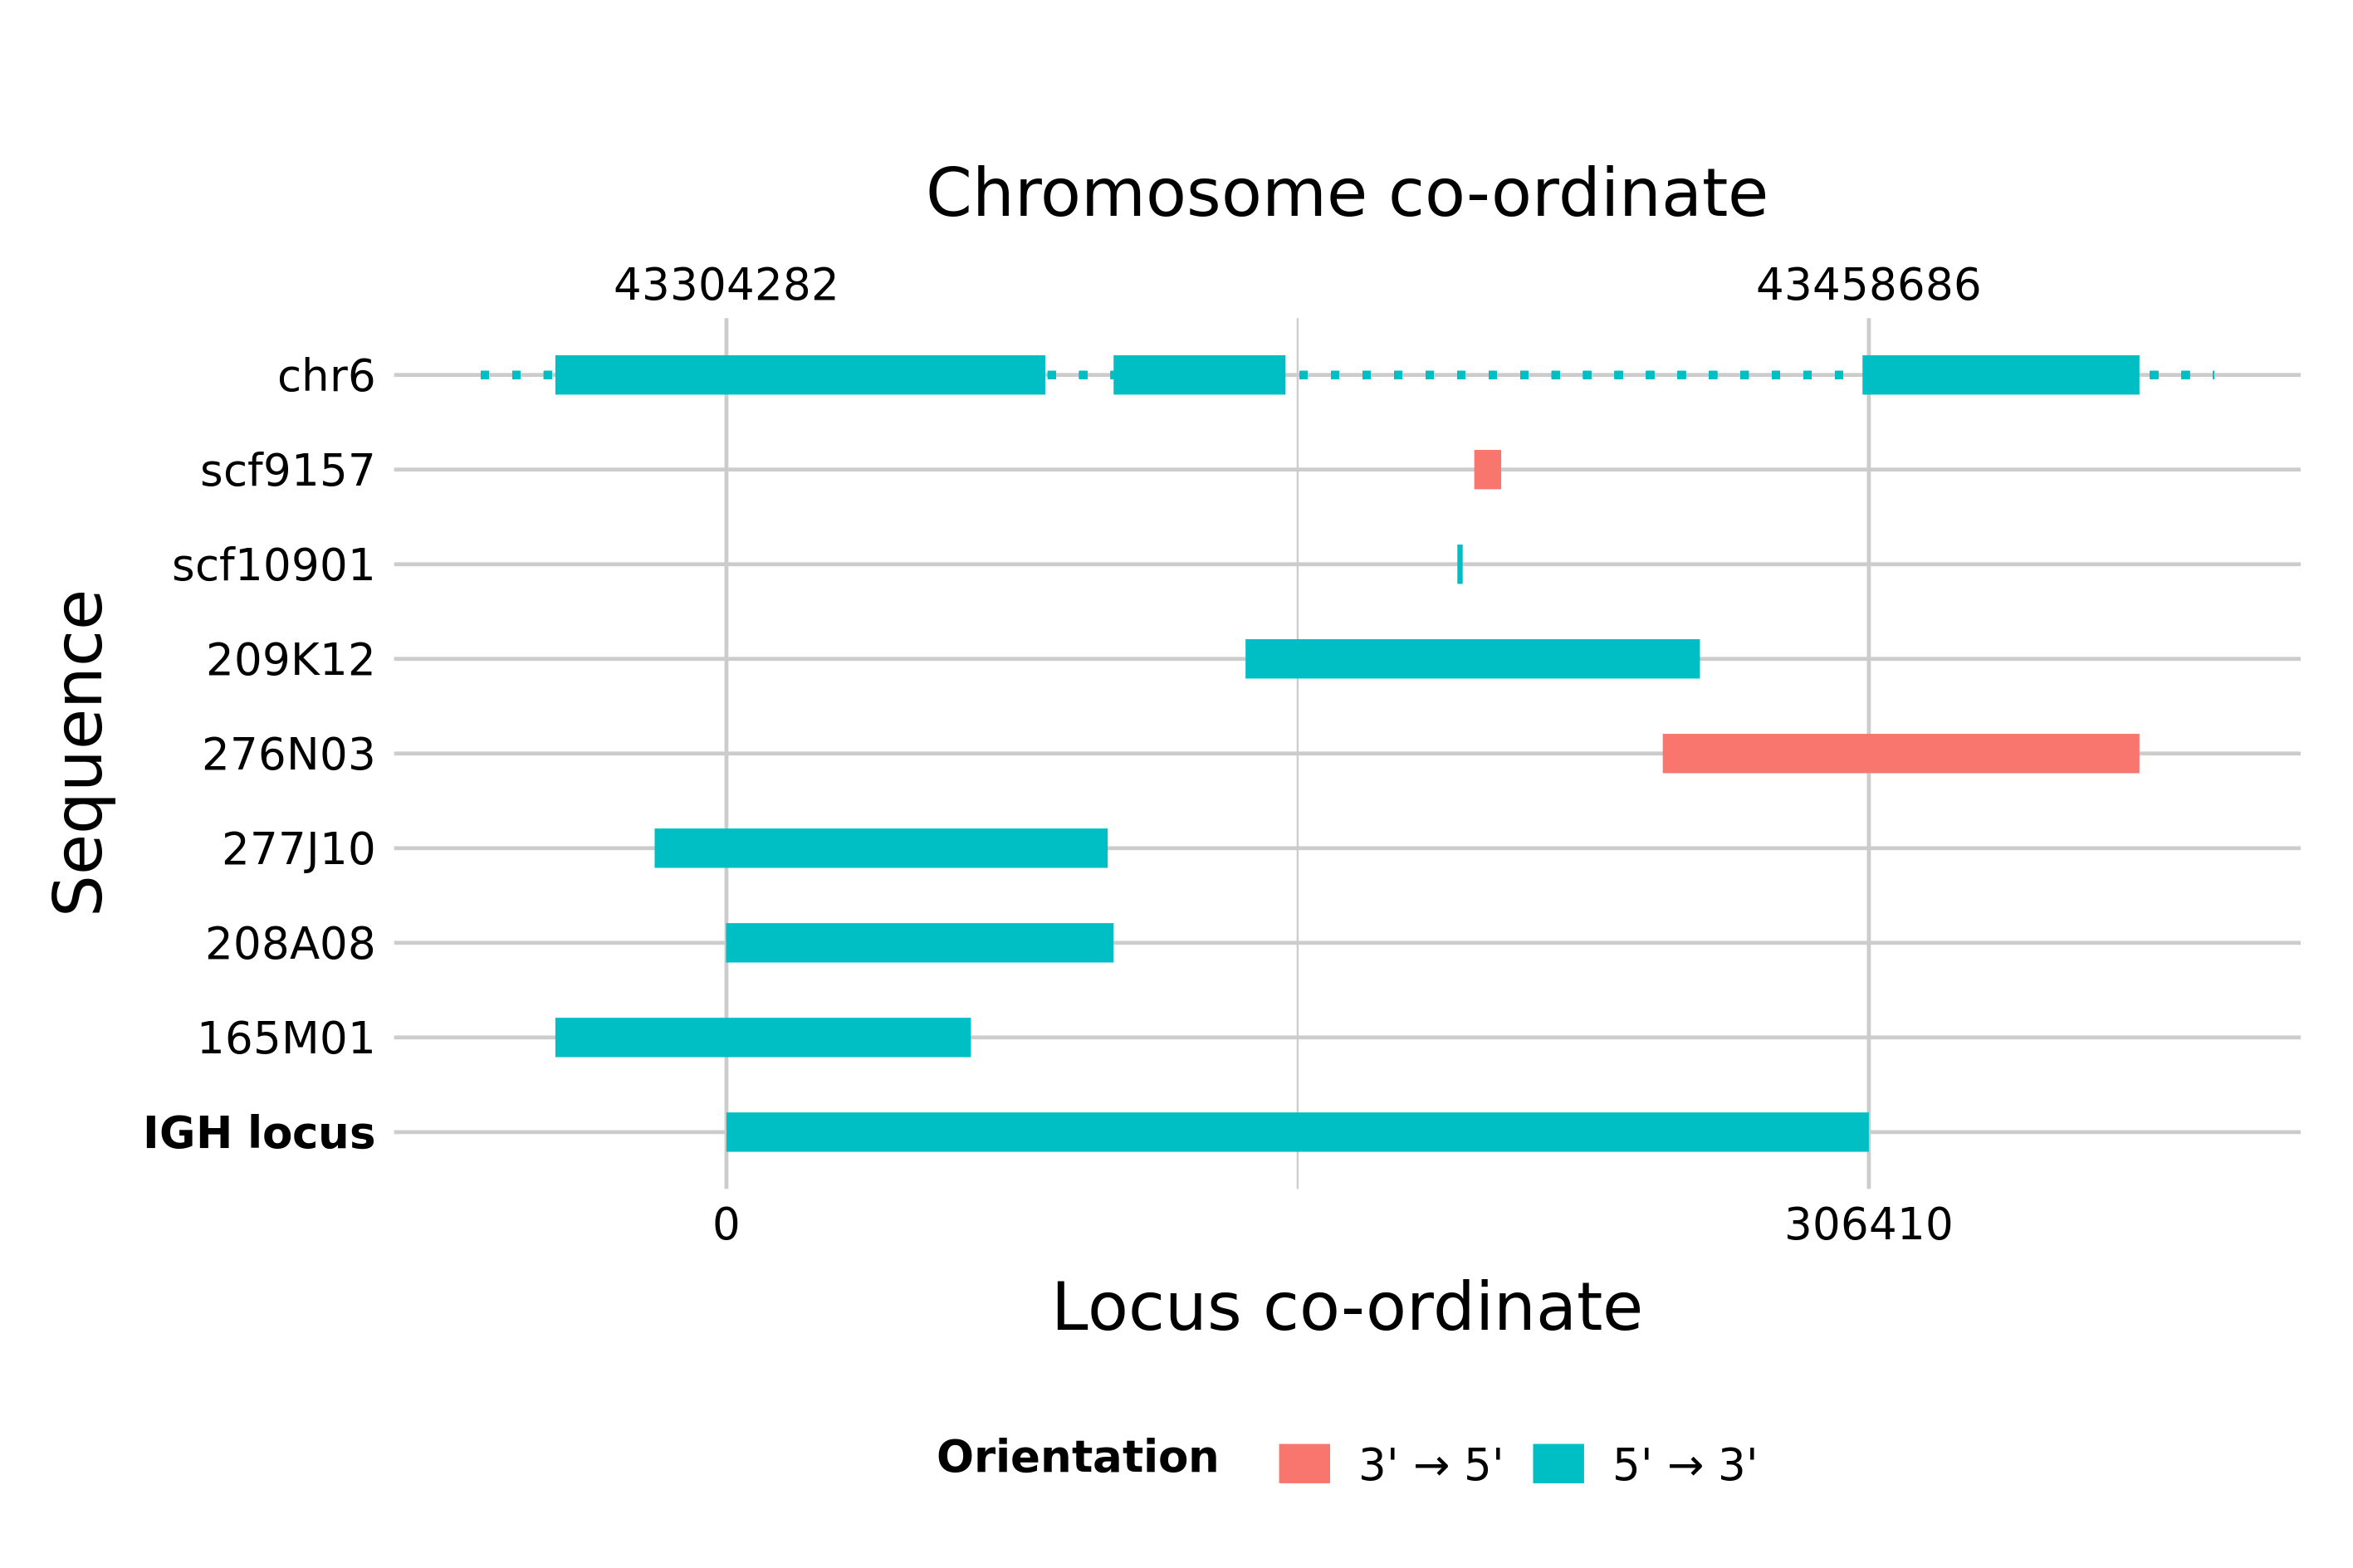
\includegraphics[width=\textwidth]{_Figures/png/nfu-locus-aln}
\Caption{Assembling the \nfu \igh{} locus}{Schematic of genome scaffolds and BAC inserts contributing to the \Nfu \igh{} locus sequence, with their corresponding place within the locus sequence (bottom axis). Internal gaps with dotted lines indicate regions on chromosome 16 with no corresponding locus sequence, as a result of intercalation of BAC or scaffold sequences.}
\label{fig:nfu-locus-aln}
\end{figure}

\subsection{Overall locus structure}
\label{sec:nfu-locus-structure}
	
The turquoise-killifish genome contains a single \igh{} locus approximately 306 kilobases in length, located on chromosome 6 of the \Nfu genome (\Cref{fig:nfu-locus-map-a}). This locus comprises two complete subloci, \igh{1} (\kb{155}) and \igh{2} (\kb{118}), present in tandem and each occupying a classic {\vh-\dh-\jh-\ch} translocon configuration. This modified translocon structure, with multiple translocon subloci present in tandem, has been observed in a number of teleost \igh{} loci including catfish, medaka and stickleback (\Cref{sec:intro_teleost_loci}) \parencite{fillatreau2013astonishing}. Unusually, however, the smaller \igh{2} sublocus in \nfu \igh{} is present in antisense relative to the larger \igh{1}, with the two subloci beginning at opposite ends of the locus and extending in opposite sense towards the middle (\Cref{fig:nfu-locus-map-b}). Such a multi-orientation structure has been seen only rarely in previously-characterised teleost \igh{} loci; to my knowledge, it has only been previously observed in medaka \parencite{magadan2011medaka} and Atlantic salmon (\Cref{fig:intro-teleost-loci-complex}). As medaka is the closest relative of the turquoise killifish to have its locus characterised prior to the present study, it is interesting to see this unusual feature reproduced here, raising the question of whether this ideosyncracy is homologous between the two loci.
	
Compared to other closely-related loci, the turquoise-killifish locus is relatively sparse, with comparatively low functional complexity given its overall size. For example, whereas the stickleback locus fits four subloci, 49 \vh segments and 10 constant regions into c. \kb{200} \parencite{bao2010stickleback,gambondeza2011stickleback}, the turquoise-killifish locus, despite being roughly 50\,\% longer, contains only two subloci, four constant regions and 24 \vh segments (including pseudogenised \vh{}s). This difference is a consequence of the unusually large amount of nonfunctional sequence padding the turquoise-killifish locus, resulting in large gaps between variable segments and in some cases between constant-region exons (\Cref{fig:nfu-locus-map-b}); this high prevalence of repetitive DNA is consistent with the rest of the turquoise-killifish genome, which comprises more than 60\,\% repetitive sequence \parencite{willemsen2019popgen}, compared to just over 15\,\% in stickleback \parencite{yuan2018repeats}.
	
The two subloci in the turquoise-killifish locus are generally highly similar in their functional sequence, with a high degree of synteny between their functional regions (\Cref{fig:nfu-locus-synteny}). The greatest degree of divergence occurs in the \vh and \dh regions, with what appear to be repeated deletion events in \igh{2} resulting in a substantially lower number of \vh and \dh segments compared to \igh{1}; conversely, the \jh and constant regions are almost identical between two subloci. These patterns are discussed in more detail in \Cref{sec:nfu-locus-constant,sec:nfu-locus-variable}.
	
\begin{figure}
	\centering
	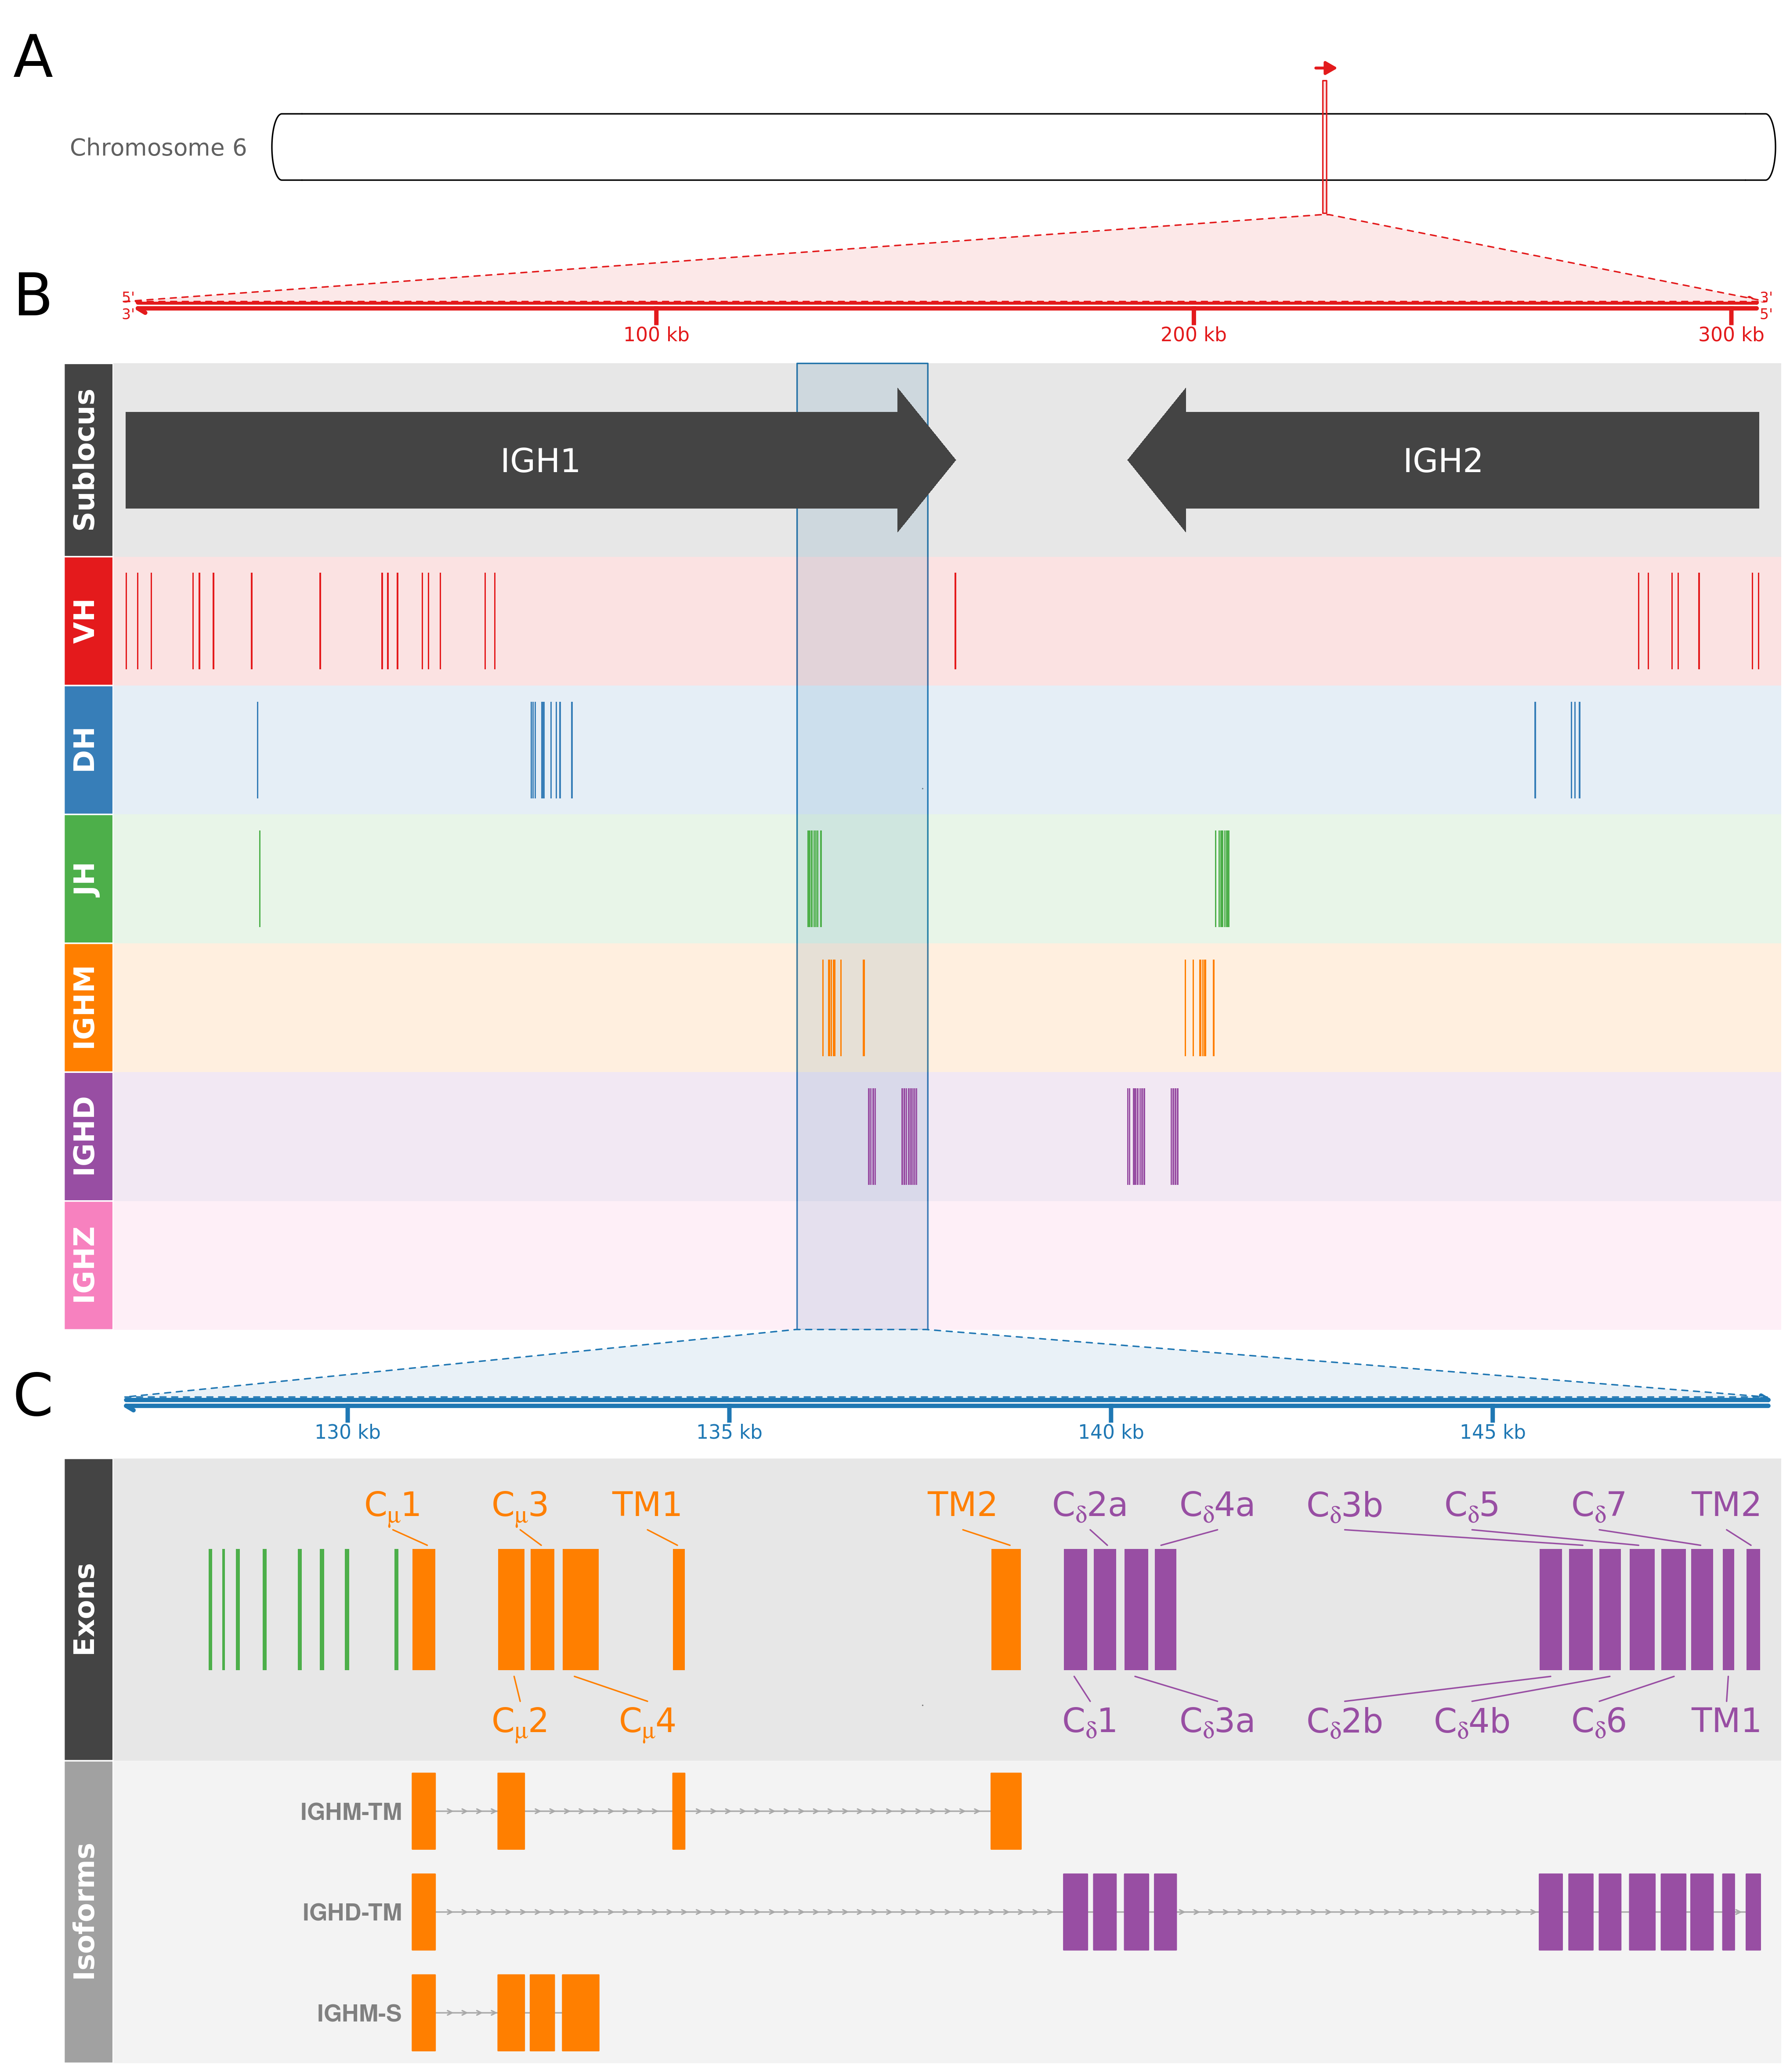
\includegraphics[width=\textwidth]{_Figures/png/nfu-locus-map}
			    \begin{subfigure}{0em}
        \phantomsubcaption{}
        \label{fig:nfu-locus-map-a}
    \end{subfigure}
    \begin{subfigure}{0em}
        \phantomsubcaption{}
        \label{fig:nfu-locus-map-b}
    \end{subfigure}
    \begin{subfigure}{0em}
        \phantomsubcaption{}
        \label{fig:nfu-locus-map-c}
        \end{subfigure}
	\Caption{The immunoglobulin heavy chain (\igh{}) locus in \nfu}{(A) Position of the \igh{} locus on chromosome 6 of the \Nfu genome. (B) Arrangement of \vh, \dh, \jh and constant-region gene segments on the \Nfu \igh{} locus. All segments follow the orientation of their parent sublocus, indicated in the uppermost track. (C) Detailed map of the constant regions of the \igh{1} sublocus, indicating the position and identity of the constant-region exons and the exon composition of expressed \igh{} isoforms in the turquoise killifish.}
	\label{fig:nfu-locus-map}
	\end{figure}
	
\begin{figure}
	\centering
	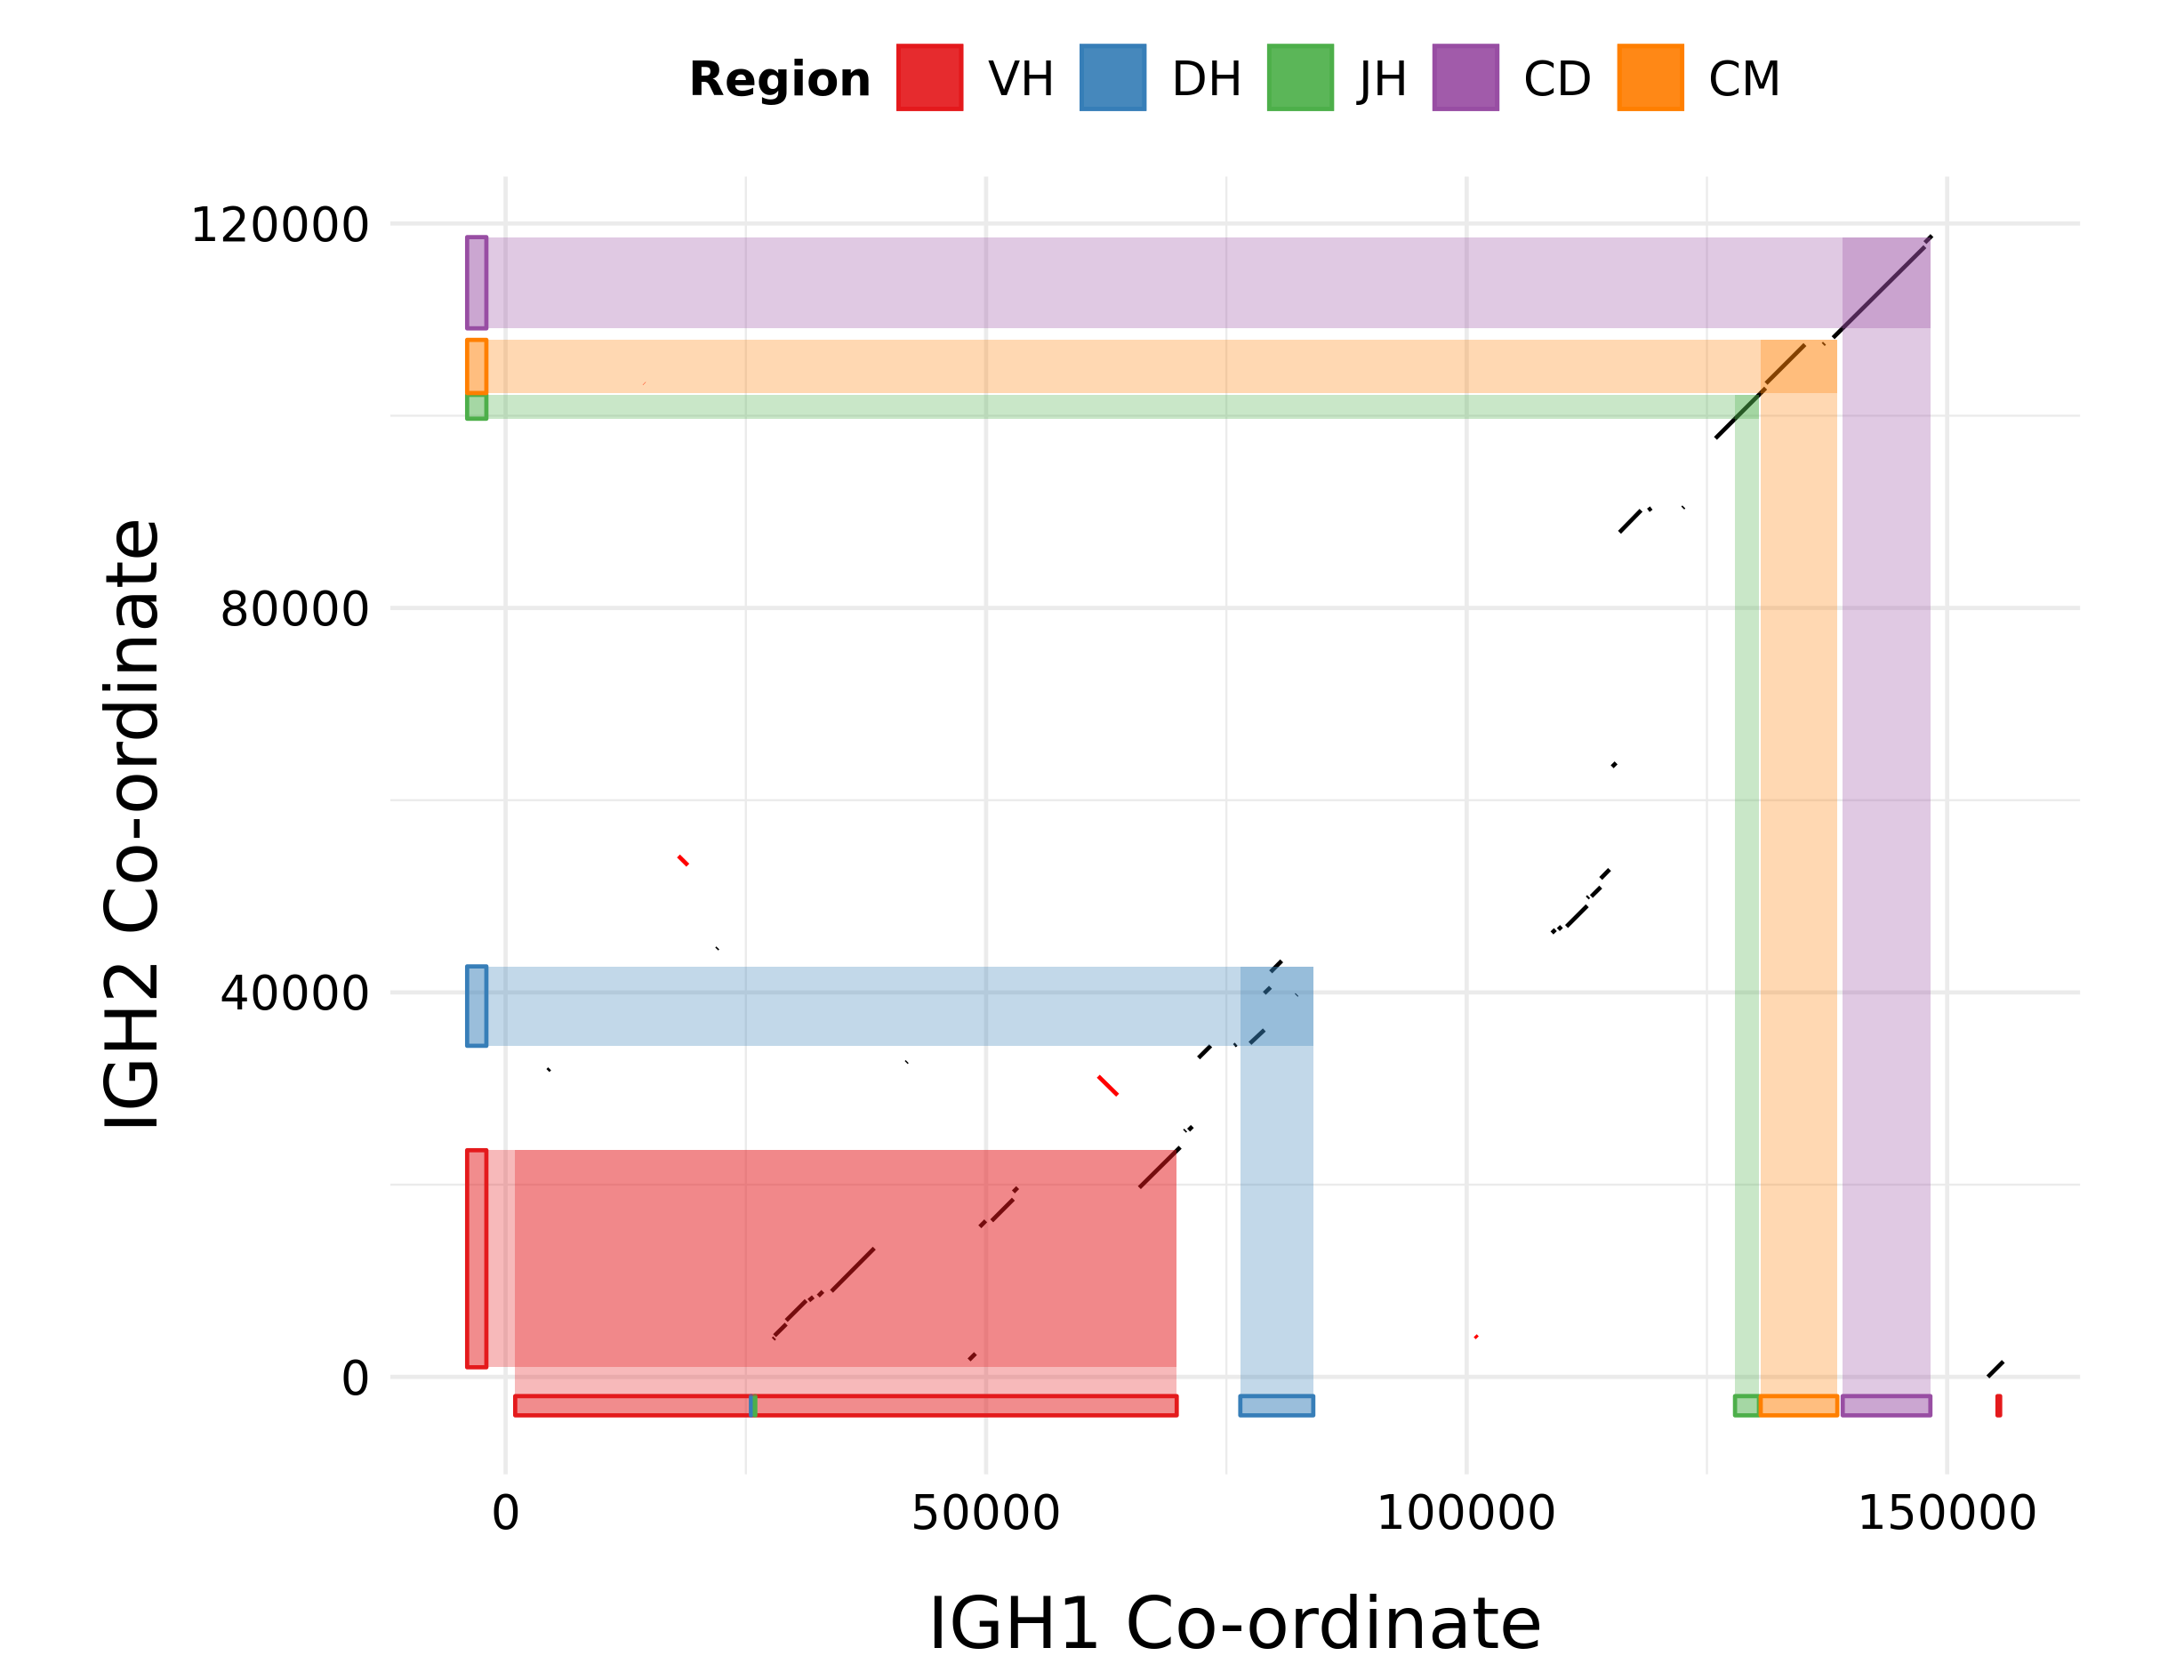
\includegraphics[width=0.9\textwidth]{_Figures/png/nfu-locus-dots}
	\Caption{Sequence homology between subloci in \Nfu \igh{}}{Synteny dot plot of sequential best matches between \igh{1} and \igh{2} subloci, with gene segment regions indicated by coloured rectangles along each axis.}
	\label{fig:nfu-locus-synteny}
\end{figure}
	
	\subsection{Constant regions}
	\label{sec:nfu-locus-constant}
	
	The isotype of an antibody determines its functional role within the immune system, including its possible effector functions and whether it can be secreted (\Cref{sec:intro_antibody_structure}) \parencite{schroeder2010immunoglobulins}. Three antibody isotypes have been identified to date in teleost fishes: \igh{M}, \igh{D} and \igh{Z} (a.k.a. \igh{T}, \igh{T/Z} or \igh{Z/T}) \parencite{fillatreau2013astonishing,bengten2015fishantibodies,magadan2015fishrepertoires}. Of these, \igh{M} and \igh{D} are highly primitive within the jawed vertebrates and found in most or all other vertebrate groups; within the teleosts, both appear to be universal \parencite{bengten2015fishantibodies}. Conversely, \igh{Z} is a teleost-specific isotype which is absent in other vertebrate taxa; within the teleosts, most characterised \igh{} loci possess \igh{Z}, but at least two (medaka and channel catfish) have been found to lack it \parencite{fillatreau2013astonishing,bengten2015fishantibodies}. In rainbow trout, \igh{Z} has been found to play a specialised mucosal role in the immune system analagous to that of \igh{A} in mammals \parencite{zhang2010igtgut,xu2013igtskin}, and it is widely assumed to play this specialised role throughout the teleosts; it is as yet unclear how mucosal immunity is effected in species lacking \igh{Z} (\Cref{sec:intro_antibody_structure}).

In order to investigate constant regions in the \nfu \igh{} locus, I identified putative exon sequences using \program{BLAST} alignments to the reference sequence databases described in \Cref{sec:nfu-locus-assembly}. Intron/exon bounderies were refined through alignment of published RNA-sequencing data from turquoise-killifish gut (\parencite{smith2017microbiota}, BioProject accession PRJNA379208, young and old untreated groups, \Cref{tab:rnaseq-sources}) using \program{STAR} (\Cref{sec:methods_comp_locus_segments} and \Cref{fig:nfu-locus-sashimi}). Strikingly, the \nfu \igh{} locus appears to completely lack any \igh{Z} constant region, with no \cz{} exons or \igh{Z} transmembrane exons being found on either \igh{1} or \igh{2}. Given the widespread prevalence and specialised mucosal role of \igh{Z} in teleosts, its surprising absence in turquoise killifish (\Cref{fig:nfu-locus-map-b}) immediately raises questions about the nature, kinetics and efficacy of mucosal adaptive immunity in this species. The similar absence of \igh{Z} in medaka, which again is the closest relative of \Nfu with a characterised locus, raises further questions about the evolutionary history of \igh{Z} in these species: does the shared absence of \igh{Z} in these species indicate a single ancestral deletion event, or parallel loss of this important isoform within both the Cyprinodontiformes (including the turquoise killifish) and the lineage leading to medaka? This latter question requires higher phylogenetic resolution to address effectively, and is investigated further in \Cref{sec:xma-locus} and \Cref{sec:locus_comparative}.
	
	While \igh{Z} is completely missing from the \Nfu \igh{} locus, \igh{M}, the most primitive and widely-found isotype in jawed vertebrates, is present in its expected location immediately downstream of the main \jh-region in both subloci. This constant region occupies the standard six-exon configuration, with four \cm{} exons and two transmembrane exons present in series on the chromosome (\Cref{fig:nfu-locus-map-b,fig:nfu-locus-map-c,fig:teleost-igm-exons-a}, \Cref{tab:nfu-ch-coords}). As with other species, both secreted and transmembrane isoforms of \igh{M} are present in the transcriptome, with secreted \igh{M} (\igh{M-S}) consisting of \cm{1-4} (\Cref{fig:nfu-locus-map-c,fig:nfu-locus-sashimi-a,fig:teleost-igm-exons-b}); however, the exon configuration of transmembrane \igh{M} (\igh{M-TM}) deviates from both that seen in mammals (in which exon TM1 is spliced to a cryptic splice site within \cm{4}) and most teleosts (in which the canonical splice site following \cm{3} is used and \cm{4} is excised) \parencite{fillatreau2013astonishing}. Rather, turquoise-killifish \igh{M-TM} resembles that of medaka, in which both \cm{3} and \cm{4} are excluded and the canonical splice site at the end of \cm{2} is spliced directly to TM1 (\Cref{fig:teleost-igm-exons-c,fig:teleost-igm-exons-d,fig:teleost-igm-exons-e}). This similarity to medaka again raises the possibility that this unusual feature may be a conserved feature of both lineages; however, the underlying mechanism giving rise to this difference in splicing behaviour is unknown.
	
		Unlike \igh{M}, the exon structure of \igh{D} is highly variable across the teleosts, ranging from roughly 7-17 \cd{} exons in addition to the transmembrane domains \parencite{fillatreau2013astonishing}. The core structure of \igh{D} comprises seven \cd{} exons (\cd{1-7}), but some subset of these exons may be missing or duplicated in any given species -- in medaka, for example, \cd{5} is missing in all subloci \parencite{magadan2011medaka}, while in many species (e.g. zebrafish, salmon, and channel catfish) \cd{2-4} are duplicated in two or more tandem blocks \parencite{fillatreau2013astonishing}. This latter configuration is also observed in turquoise killifish, in which the \igh{D} constant region immediately follows \igh{M} in both subloci and has a 

\cd{1}-(\cd{2}-\cd{3}-\cd{4})$_2$-\cd{5}-\cd{6}-\cd{7}-TM1-TM2 

	\noindent configuration, for a total of 12 exons per \igh{D} constant region (\Cref{fig:nfu-locus-map-b,fig:nfu-locus-map-c}, \Cref{tab:nfu-ch-coords}). All of these exons appear to be expressed in tandem, resulting in a much longer transcript than is observed for any isoform of \igh{M} (\Cref{fig:nfu-locus-map-c,fig:nfu-locus-sashimi-b}). As in other teleost species, \igh{D} in the turquoise killifish includes a chimeric \cm{1} exon at the 5' end of the constant-region transcript, for a total of 13 exons per \igh{D-TM} mRNA (\Cref{fig:nfu-locus-sashimi-b}).

	While the best-known form of \igh{D} in teleosts is transmembrane, secreted \igh{D} has been observed in at least two teleost species, with different mechanisms used in each case: in channel catfish, one dedicated sublocus has a dedicated \igh{D} secretory exon in place of the transmembrane exons \parencite{bengten2006catfish}, while in rainbow trout (and possibly some other species like Atlantic salmon and cod \parencite{ramirezgomez2012secretoryigd}) a run-on event at the end of \cd{7} results in the production of a secretory tail in a manner similar to secretory \igh{Z} \parencite{ramirezgomez2012secretoryigd}. However, neither a specialised secretory exon nor a \cd{7} secretory tail could be detected in turquoise killifish, suggesting that \igh{D} may only be expressed in transmembrane form in this species.
	
	In the case of both \igh{M} and \igh{D}, the constant regions are present in their expected configuration in each sublocus and are highly similar in sequence between the subloci, with an average of 98.4\,\% nucleotide sequence identity for corresponding \igh{M} exons and 99.3\,\% for corresponding \igh{D} exons (\Cref{fig:nfu-ch-aln} and \Cref{tab:nfu-ch-aln}) in pairwise Needleman-Wunsch alignments \parencite{needleman1970alignment}. This high level of similarity indicates either a very recent duplication event to produce the second sublocus or a high level of sequence conservation in both subloci, with the latter explanation suggesting that both subloci continue to be functional and active in the immune system.
	
	\begin{figure}
	\centering
		    \begin{subfigure}{0em}
        \phantomsubcaption{}
        \label{fig:teleost-igm-exons-a}
    \end{subfigure}
    \begin{subfigure}{0em}
        \phantomsubcaption{}
        \label{fig:teleost-igm-exons-b}
    \end{subfigure}
    \begin{subfigure}{0em}
        \phantomsubcaption{}
        \label{fig:teleost-igm-exons-c}
    \end{subfigure}
    \begin{subfigure}{0em}
        \phantomsubcaption{}
        \label{fig:teleost-igm-exons-d}
    \end{subfigure}
    \begin{subfigure}{0em}
        \phantomsubcaption{}
        \label{fig:teleost-igm-exons-e}
    \end{subfigure}
	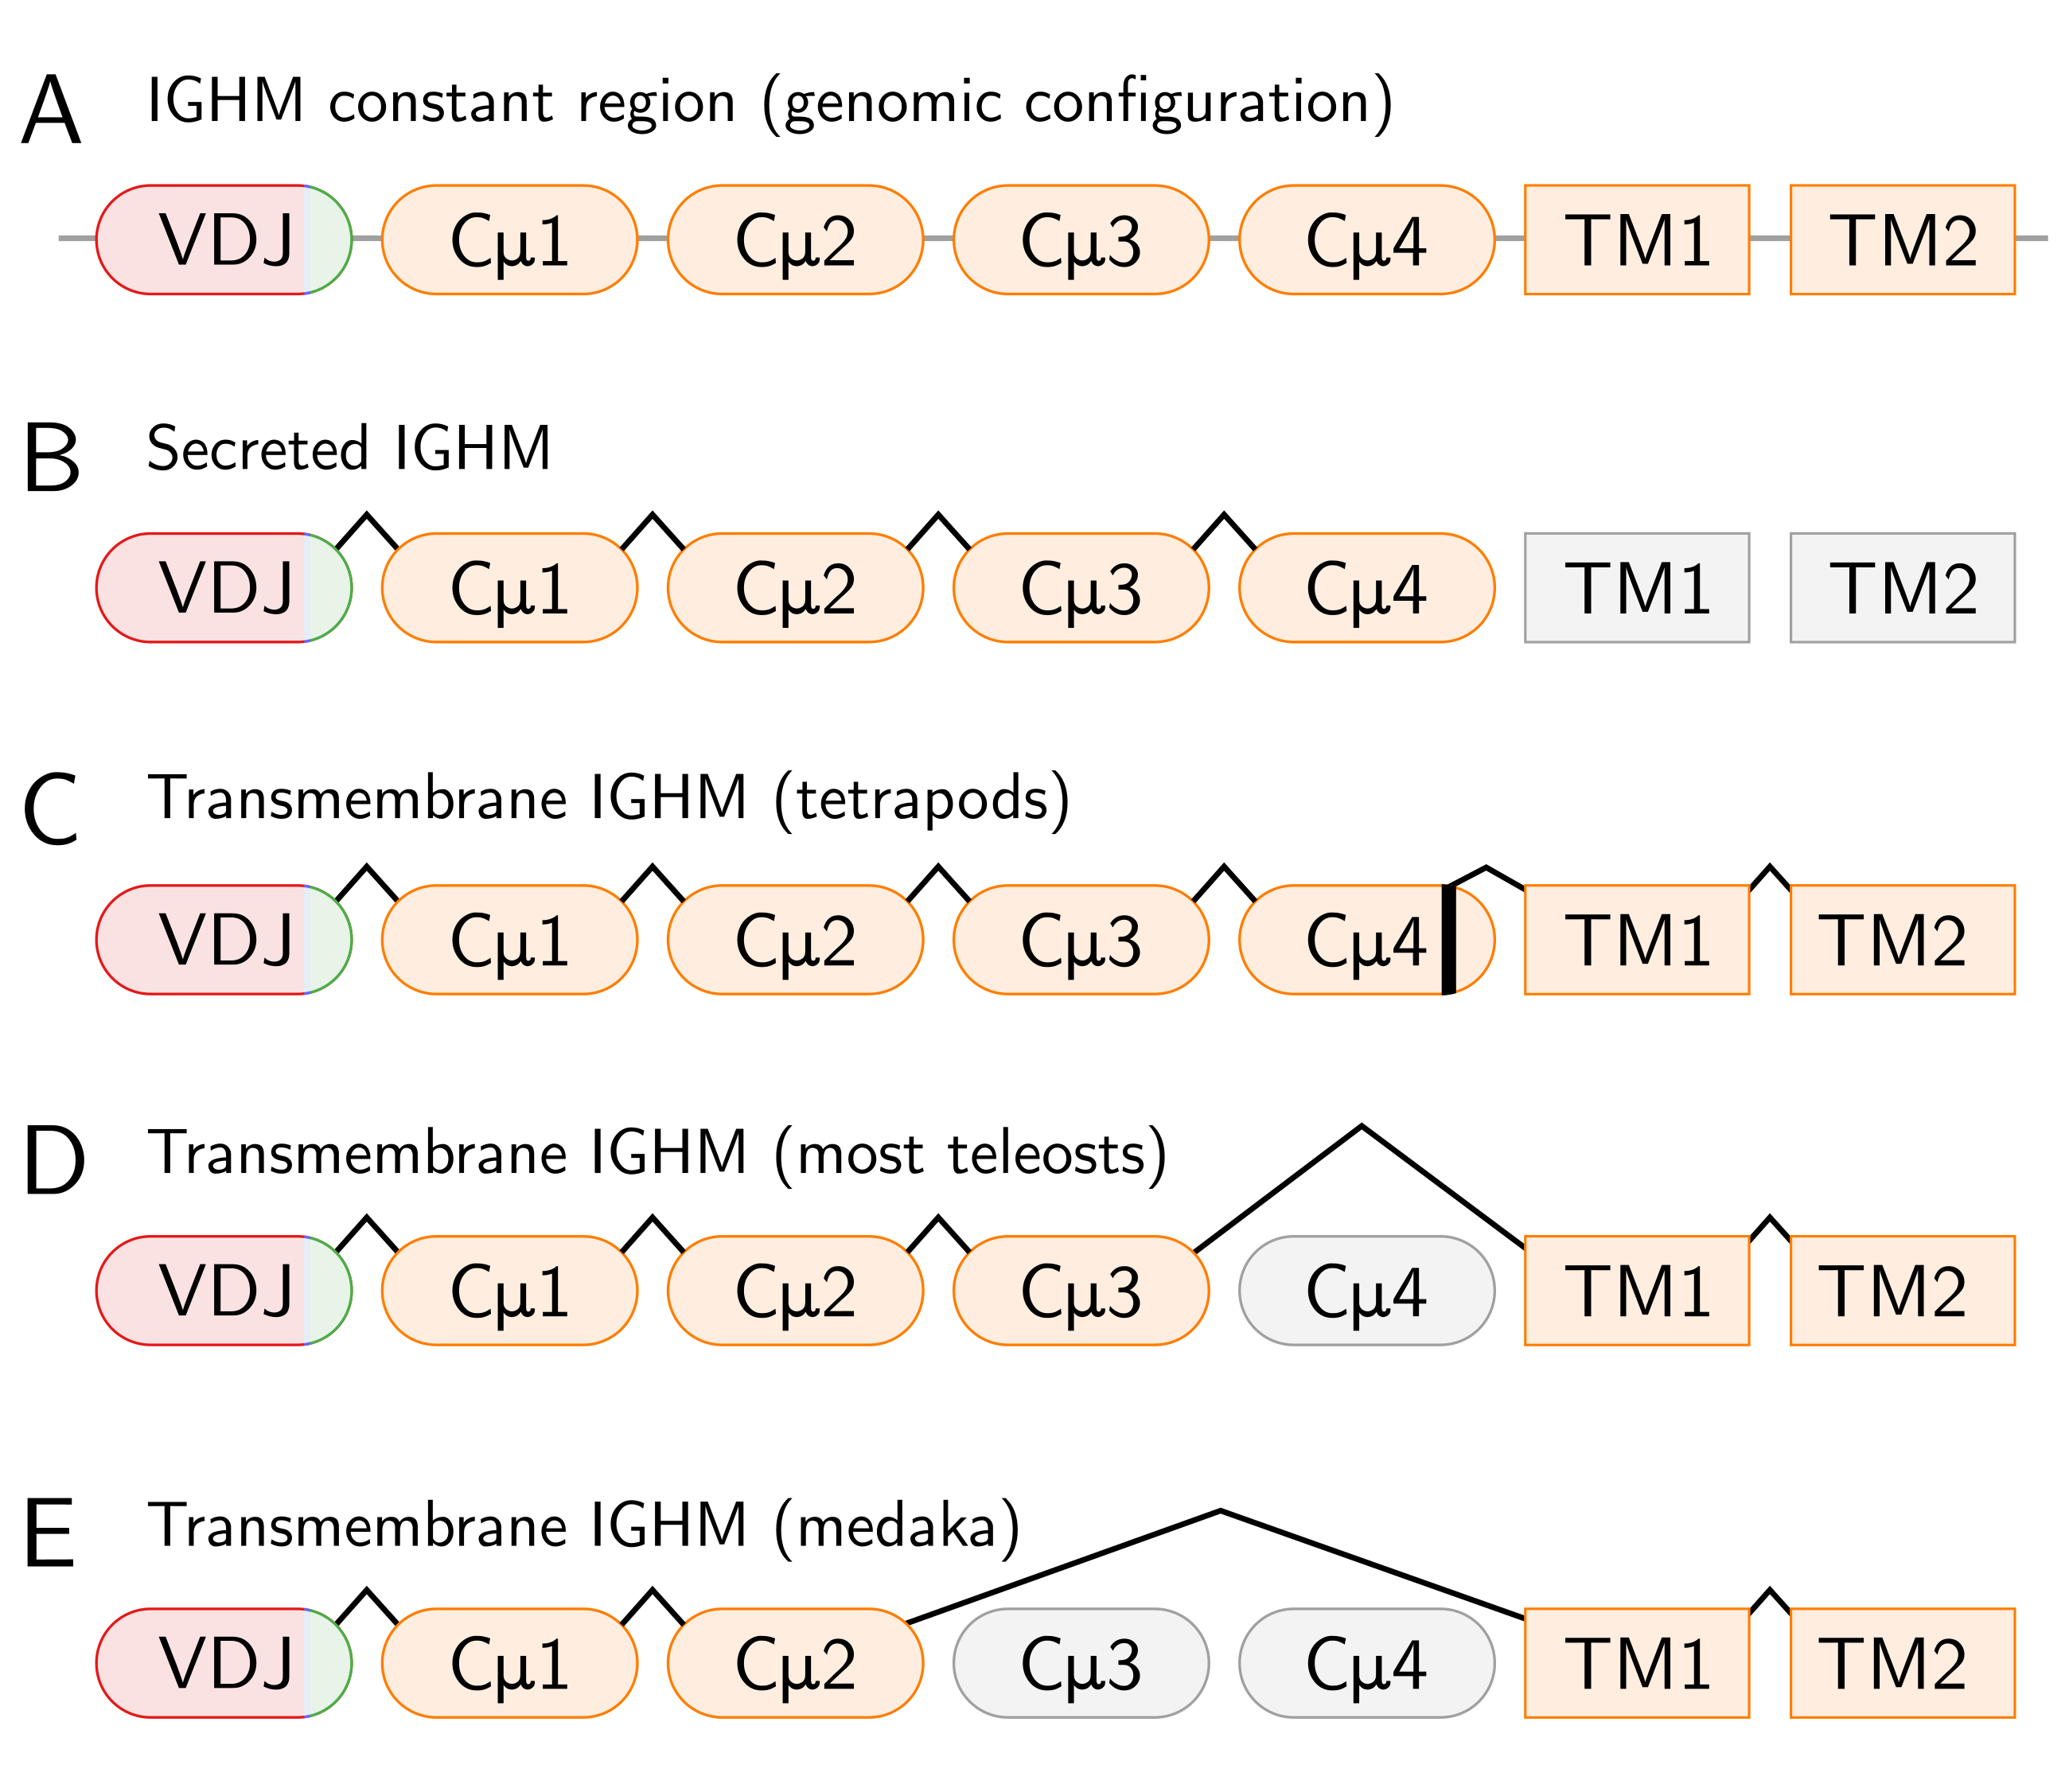
\includegraphics[width=0.8\textwidth]{_Figures/png_edited/teleost-igm-exons}
	\Caption{\igh{M} exon usage in bony vertebrates}{Schematic of \igh{M} splice patterns in different isoforms and taxonomic groups; (A) standard genomic (pre-splicing) configuration of \igh{M}, following VDJ recombination; (B) exon configuration of secreted \igh{M} (\igh{M-S}) in tetrapods and teleosts; (C) exon configuration of transmembrane \igh{M} (\igh{M-TM}) in tetrapods, demonstrating the use of a cryptic splice site in \cm{4}; (D) standard \igh{M-TM} exon configuration in teleosts, demonstrating the direct splicing of \cm{3} to TM1 and exclusion of \cm{4}; (E) unusual \igh{M-TM} exon configuration observed in medaka, in which both \cm{3} and \cm{4} are excluded. Adapted from Figure 3 of \parencite{fillatreau2013astonishing}.}
	\label{fig:teleost-igm-exons}
	\end{figure}
	
	\begin{figure}
	\centering
		\begin{subfigure}{0em}
        \phantomsubcaption{}
        \label{fig:nfu-locus-sashimi-a}
    \end{subfigure}
    \begin{subfigure}{0em}
        \phantomsubcaption{}
        \label{fig:nfu-locus-sashimi-b}
    \end{subfigure}
	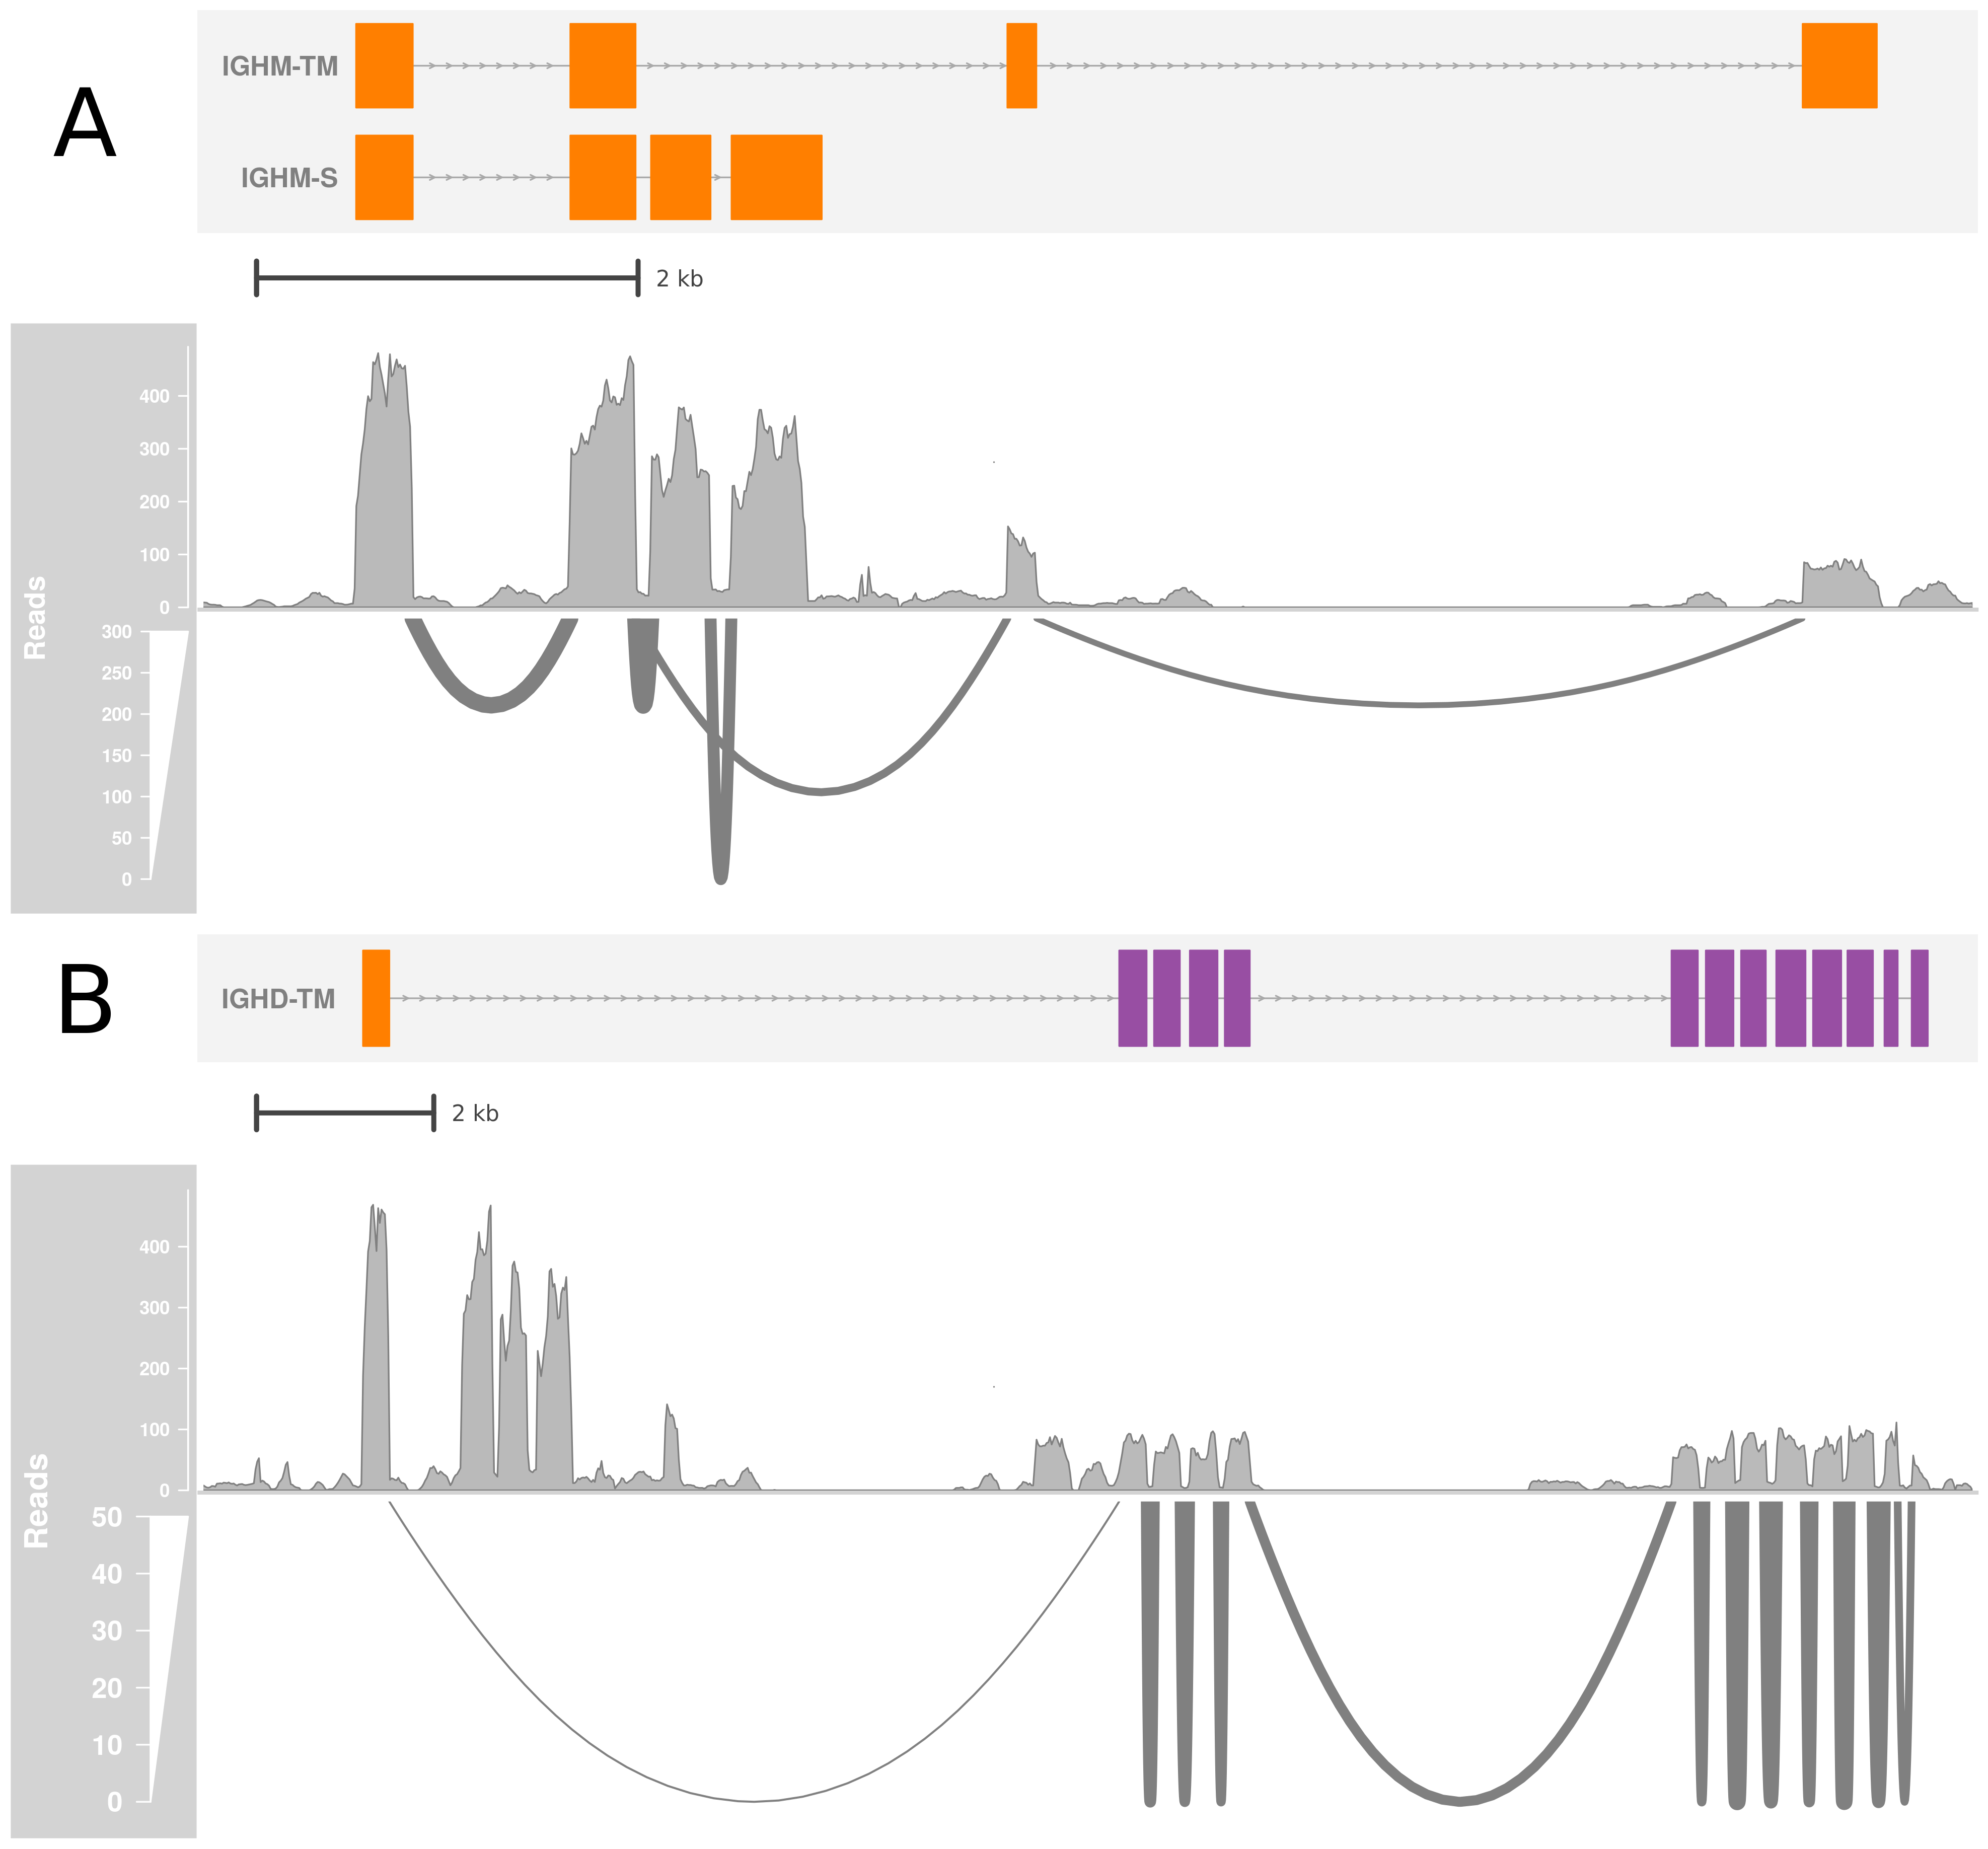
\includegraphics[width=\textwidth]{_Figures/png/nfu-locus-sashimi}
	\Caption{Constant-region isoforms in \Nfu}{Coverage and Sashimi plots \parencite{katz2013sashimi} of \program{STAR}-aligned RNA-seq reads from \Nfu gut samples \parencite{smith2017microbiota}, demonstrating the splicing behaviour of \igh{1} constant-region isoforms and showing the read coverage of each exon and splice junction. (A) \igh{M} exon splicing, showing alternative splicing patterns of \igh{M-TM} and \igh{M-S}; (B) \igh{D} exon splicing, showing chimeric splicing of \cm{1} to \cd{1}.}
	\label{fig:nfu-locus-sashimi}
	\end{figure}
	
	\begin{figure}
	\centering
	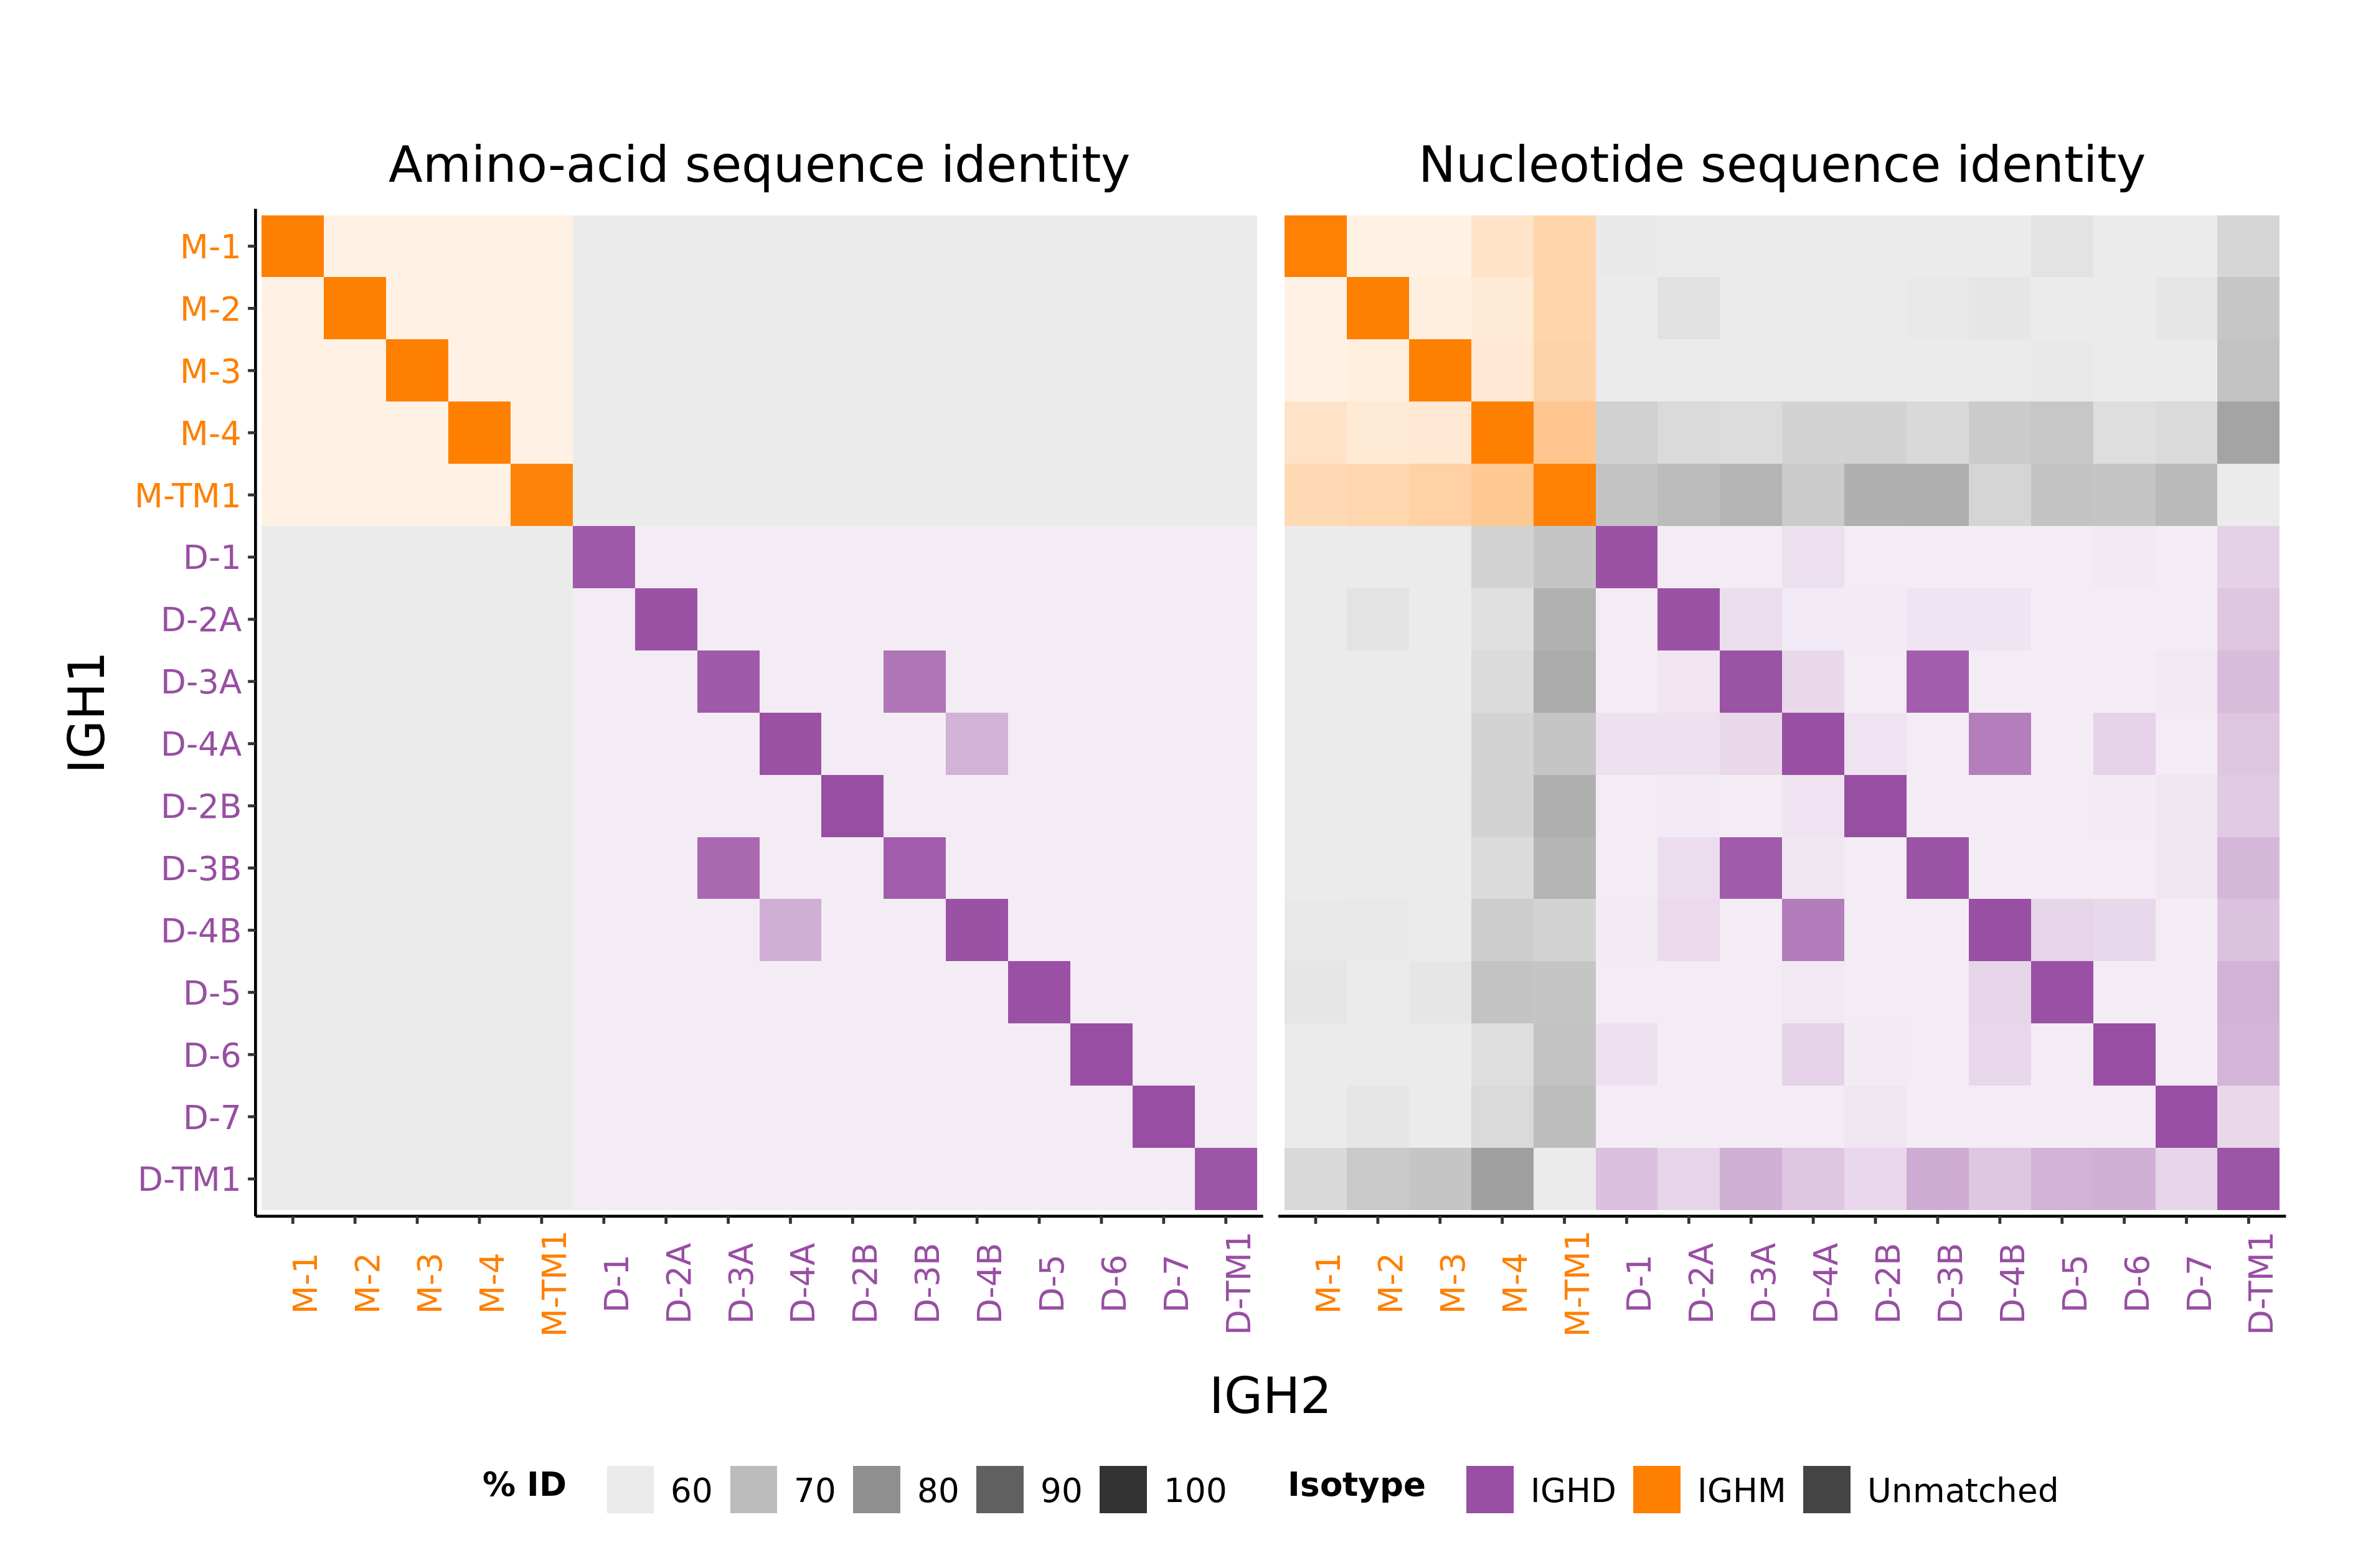
\includegraphics[width = \textwidth]{_Figures/png/nfu-ch-aln}
	\Caption{Cross-sublocus sequence similarity of constant-region exons in \Nfu \igh{}}{Heatmap of percentage sequence identity between amino-acid (left) and nucleotide (right) sequences of constant-region exons (excluding \igh{M-TM2} and \igh{D-TM2}) from the two subloci of \Nfu \igh{}, calculated using pairwise Needleman-Wunsch global alignments.}
	\label{fig:nfu-ch-aln}
	\end{figure}
	
	\begin{table}\centering
		\Caption{Cross-sublocus sequence similarity of constant-region exons in \Nfu}{Percentage sequence identities of pairwise Needleman-Wunsch global alignments between nucleotide (NT) or amino-acid (AA) sequences of corresponding exons from the two subloci of \Nfu \igh{}.}
	% latex table generated in R 3.5.1 by xtable 1.8-3 package
% Wed Dec 19 17:33:43 2018
\begin{tabular}{llrr}
  \toprule Isotype & Exon & NT & AA \\ 
  \midrule M & 1 & 99.66 & 100.00 \\ 
  M & 2 & 100.00 & 100.00 \\ 
  M & 3 & 100.00 & 100.00 \\ 
  M & 4 & 100.00 & 100.00 \\ 
  M & TM1 & 99.34 & 98.00 \\ 
  M & TM2 & 91.67 & 100.00 \\ 
  D & 1 & 99.03 & 97.06 \\ 
  D & 2A & 98.97 & 98.96 \\ 
  D & 3A & 98.72 & 97.09 \\ 
  D & 4A & 99.65 & 98.92 \\ 
  D & 2B & 100.00 & 100.00 \\ 
  D & 3B & 98.72 & 96.12 \\ 
  D & 4B & 99.64 & 98.91 \\ 
  D & 5 & 99.09 & 99.08 \\ 
  D & 6 & 100.00 & 100.00 \\ 
  D & 7 & 100.00 & 100.00 \\ 
  D & TM1 & 97.99 & 97.96 \\ 
  D & TM2 & 99.44 & 100.00 \\ 
   \bottomrule \end{tabular}

	\label{tab:nfu-ch-aln}
	\end{table}
	
\subsection{Variable regions}
\label{sec:nfu-locus-variable}
	
Variable-region gene segments in the turquoise-killifish \igh{} locus were identified with a variety of methods, depending on the type of gene segment being analysed (\Cref{sec:methods_comp_locus_segments}). \vh candidates were identified probabilistically using Hidden Markov Models constructed by \program{nhmmer} \parencite{wheeler2013nhmmer} from \program{PRANK} \parencite{loytynoja2014prank} multiple-sequence alignments of reference sequences, with the 3'-ends of each V-exon identified by the presence of a recombination-signal sequence (RSS) \parencite{schroeder2010immunoglobulins} and the 5'-ends refined using \program{IMGT-DomainGapAlign} \parencite{ehrenmann2011domaingapalign}. \jh candidates were also identified using \program{nhmmer}, with segment ends identified by the presence of an RSS (5') and a \sequence{GTA} splice-site motif (3') \parencite{magadan2011medaka}. Finally, \dh-segments, being too short and variable in sequence for HMM-based approaches to be effective, were identified by searching for pairs of flanking RSS sequences in opposite orientation, using fuzzy pattern-matching (with EMBOSS \program{FUZZNUC} \parencite{rice2000emboss}) to conserved RSS sequence motifs.
	 
In total, I identified 24 \vh-segments, 14 \dh-segments and 17 \jh-segments in the \Nfu locus (\Cref{tab:nfu-vh-coords,tab:nfu-dh-coords-seg,tab:nfu-jh-coords-seg}), of which the majority (17 \vh, 10 \dh and 8 \jh) were present in \igh{1}. Of the \vh segments identified, three contain premature stop codons, though none is out-of-frame; conversely, all the \dh and \jh segments identified appear to be in-frame and functional, with no premature stop codons. However, in all cases a minority of segments contain RSS sequences that deviate significantly from the expected consensus sequence (\Cref{tab:nfu-vh-coords,tab:nfu-dh-coords-rss5,tab:nfu-dh-coords-rss3,tab:nfu-jh-coords-rss}); it is unclear whether these sequences can recombine to successfully produce mature VDJ sequences \textit{in vivo}. In the case of the \vh segments, of the six sequences without clearly functional RSS sequences, three also contain premature stop codons, suggesting the changes to the RSS in these cases may arise from relaxed purifying selection on already-pseudogenised sequences.

Apart from these few exceptions, however, the recombination signal sequences (RSS) marking the ends of the \vh, \dh and \jh gene segments in the \Nfu locus otherwise strongly resemble those of other characterised teleosts, which in turn resemble those of non-teleost loci (\Cref{fig:nfu-rss-seqlogo-all,fig:nfu-rss-seqlogo-sep}). The overall heptamer and nonamer consensus sequences (\texttt{CACAGTG} for heptamers and \texttt{ACAAAAACC} for nonamers) closely matched those expected from the literature \parencite{schroeder2010immunoglobulins}, while in 88\,\% of cases the spacer region was within 1bp of the expected length (12bp for \dh-RSSs, 23bp for \vh- and \jh-RSSs); interestingly, the greatest number of \vh-RSSs had a 22bp (rather than 23bp) spacer, but this is unlikely to interfere with RSS functionality. Overall, the RSSs in the turquoise killifish appear to be supporting the normal operation of VDJ-recombination in this species.

Of the \vh, \dh and \jh segments identified, all but one of each type of segment is located within contiguous V-, D-, and J-regions within each sublocus, supporting a modified translocon configuration for turquoise-killifish \igh. The exceptions to this are \igh{1D01} and \igh{1J01}, which are embedded within the \igh{1} V-region, and a single \vh segment located in between the \igh{D} constant regions of the two subloci (\Cref{fig:nfu-locus-map-b}). The unusual location of \igh{1D01} and \igh{1J01} may represent the result of a transposition event within the \igh{} locus; however, their close colocalisation and 5' position within the \igh{1} sublocus, as well as the fact that neither has a close paralogue in \igh{2} (\Cref{fig:nfu-dj-alignment-b}), suggest that they may instead represent the remnant of a formerly present \igh{Z} constant region, as these typically have dedicated D/J segments independent of those serving \igh{M} (\Cref{sec:intro_teleost_loci}). Given its forward orientation, meanwhile, I assigned the orphaned \vh-segment to the \igh{1} sublocus as \igh{1V1-07}; however, if annotated correctly, it is unlikely to successfully recombine with segments in either sublocus due to its unusual location.
		
\begin{table}[hb]
	\centering
	\begin{threeparttable}
	\centering
	\caption{Number of functional \vh-segments and \vh-families in other teleost species}
	\label{tab:teleost-vh-counts}
	\begin{tabular}{ccccc}\toprule
	\multirow{2}{*}{	\textbf{Common Name}} & \multirow{2}{*}{\textbf{Species}} & \textbf{\# Functional} & \textbf{	\# \vh} & \multirow{2}{*}{\textbf{Source}} \\
	& & \textbf{\vh Segments} & \textbf{Families} & \\\midrule
	Zebrafish & \textit{Danio rerio} & 39 & 13\,\tnote{1} & \parencite{magadan2015fishrepertoires} \\
	Grass carp & \textit{Ctenopharyngodon idella} & 8 & 5\,\tnote{2} & \parencite{xiao2010grasscarp} \\
	Fugu & \textit{Takifugu rubripes} & 34 & 3 & \parencite{magadan2015fishrepertoires} \\
	Medaka & \textit{Oryzias latipes} & 35 & 6 & \parencite{fillatreau2013astonishing,magadan2011medaka} \\
	Stickleback & \textit{Gasterosteus aculeatus} & 49 & 4 & \parencite{magadan2015fishrepertoires} \\
	Turquoise killifish & \textit{Nothobranchius furzeri} & 21\,\tnote{3} & 6 & -- \\
	\bottomrule\end{tabular}
	\begin{tablenotes}
	\item[1] \vh families in zebrafish were identified based on 70\,\% (rather than 80\,\%) sequence identity.
	\item[2] It is not clear what clustering method or threshold was used to identify \vh families in grass carp.
	\item[3] Excluding \vh segments with nonsense or frameshift mutations, but not those with uncertain or missing RSS sequences.
	\end{tablenotes}
	\end{threeparttable}
\end{table}
	
\vh sequences within an \igh{} locus are conventionally grouped into families on the basis of nucleotide sequence identity, with a typical identity cutoff of 80\,\% \parencite{magadan2015fishrepertoires}. In order to group the \Nfu \vh genes into families, I performed pairwise Needleman-Wunsch global alignments on each pair of \vh sequences to obtain pairwise identity scores, followed by single-linkage clustering on the resulting identity matrix (\Cref{sec:methods_comp_locus_segments}). Cutting the dendrogram at 80\,\% sequence identity revealed a total of six \vh families, of which four contained more than one \vh segment (\Cref{fig:nfu-vh-families}); this number of \vh families in the \Nfu locus is roughly in line with those found in related species (\Cref{tab:teleost-vh-counts}). Of these, V1 and V2 make up the bulk (42\,\% and 29\,\% respectively) of the \vh segments in the locus. V2 and V4 are highly similar, and all the members of V4 are pseudogenised by premature stop codons; it may therefore be more appropriate to regard V4 as a pseudogenised subfamily of V2 than as a \vh family in its own right.

The total number of functional \vh segments in the turquoise-killifish locus is unusually small in comparison to the total numbers observed in many other teleost species (\Cref{tab:teleost-vh-counts}); however, the number of segments per sublocus is in line with the numbers seen in closely-related species (2 to 12 in medaka \parencite{magadan2011medaka}, 6 to 18 in stickleback \parencite{gambondeza2011stickleback,bao2010stickleback}), with the overall difference mainly arising from a difference in the number of subloci per locus. A similar pattern is observed with \jh segments, with similar numbers of segments per sublocus in turquoise killifish and closely-related species, especially medaka. It therefore appears that the per-sublocus segment diversity available to the turquoise killifish is similar to that of previously characterised species, with any difference in total available diversity at this level arising from differences in the number of functional subloci rather than the size of the V/D/J-regions \textit{per se}.

As can be seen from \Cref{fig:nfu-locus-synteny}, much of the V-, D- and especially J-region sequence in the \Nfu locus is syntenic between the two \igh{} subloci, with downstream portions of the \igh{2} V-region corresponding to downstream parts of the \igh{1} region. Of the seven \vh segments in \igh{2}, six have a corresponding segment on \igh{1} with which they share at least 97\,\% sequence identity (\Cref{fig:nfu-vh-families}), and these partner segments are largely (though not entirely) colinear in their ordering between the two subloci. A similar pattern can be observed for the D- and (especially) the J-regions: of the four \dh segments detectable in \igh{2}, three (\igh{2D02} to \igh{2D04}) are identical with another block of adjacent \dh segments in \igh{1} (\igh{1D05} to \igh{1D07}), while the \jh-regions exhibit almost complete sequence identity between the eight \jh segments of the main \jh region in \igh{1} and the eight \jh segments in \igh{2} (\Cref{fig:nfu-dj-alignment}).
		
Nevertheless, as is clear from \Cref{fig:nfu-locus-synteny}, there are large portions the \igh{1} variable region, including the first 25 kilobases of the V-region, for which no corresponding sequence exists in \igh{2}, and there are many \vh and \dh segments in \igh{1} (and a much smaller number in \igh{2}) for which no close homologue exists in the other sublocus. Taken together, these data are consistent with a model in which \igh{2} was produced via duplication and inversion of all or part of \igh{1}, followed by subsequent deletion events in the redundant, and structurally volatile, \igh{2} \vh and \dh regions. However, it is not clear at present how to distinguish between this model and an alternative one of expansion in \igh{1}, or how to explain why the \jh region is so much more conserved between subloci than either the \vh or \dh regions.

	
	\begin{figure}
	\centering
	\begin{subfigure}{0em}
	\phantomsubcaption{}
    \label{fig:nfu-vh-families-a}
    \end{subfigure}
    \begin{subfigure}{0em}
    \phantomsubcaption{}
    \label{fig:nfu-vh-families-b}
    \end{subfigure}
	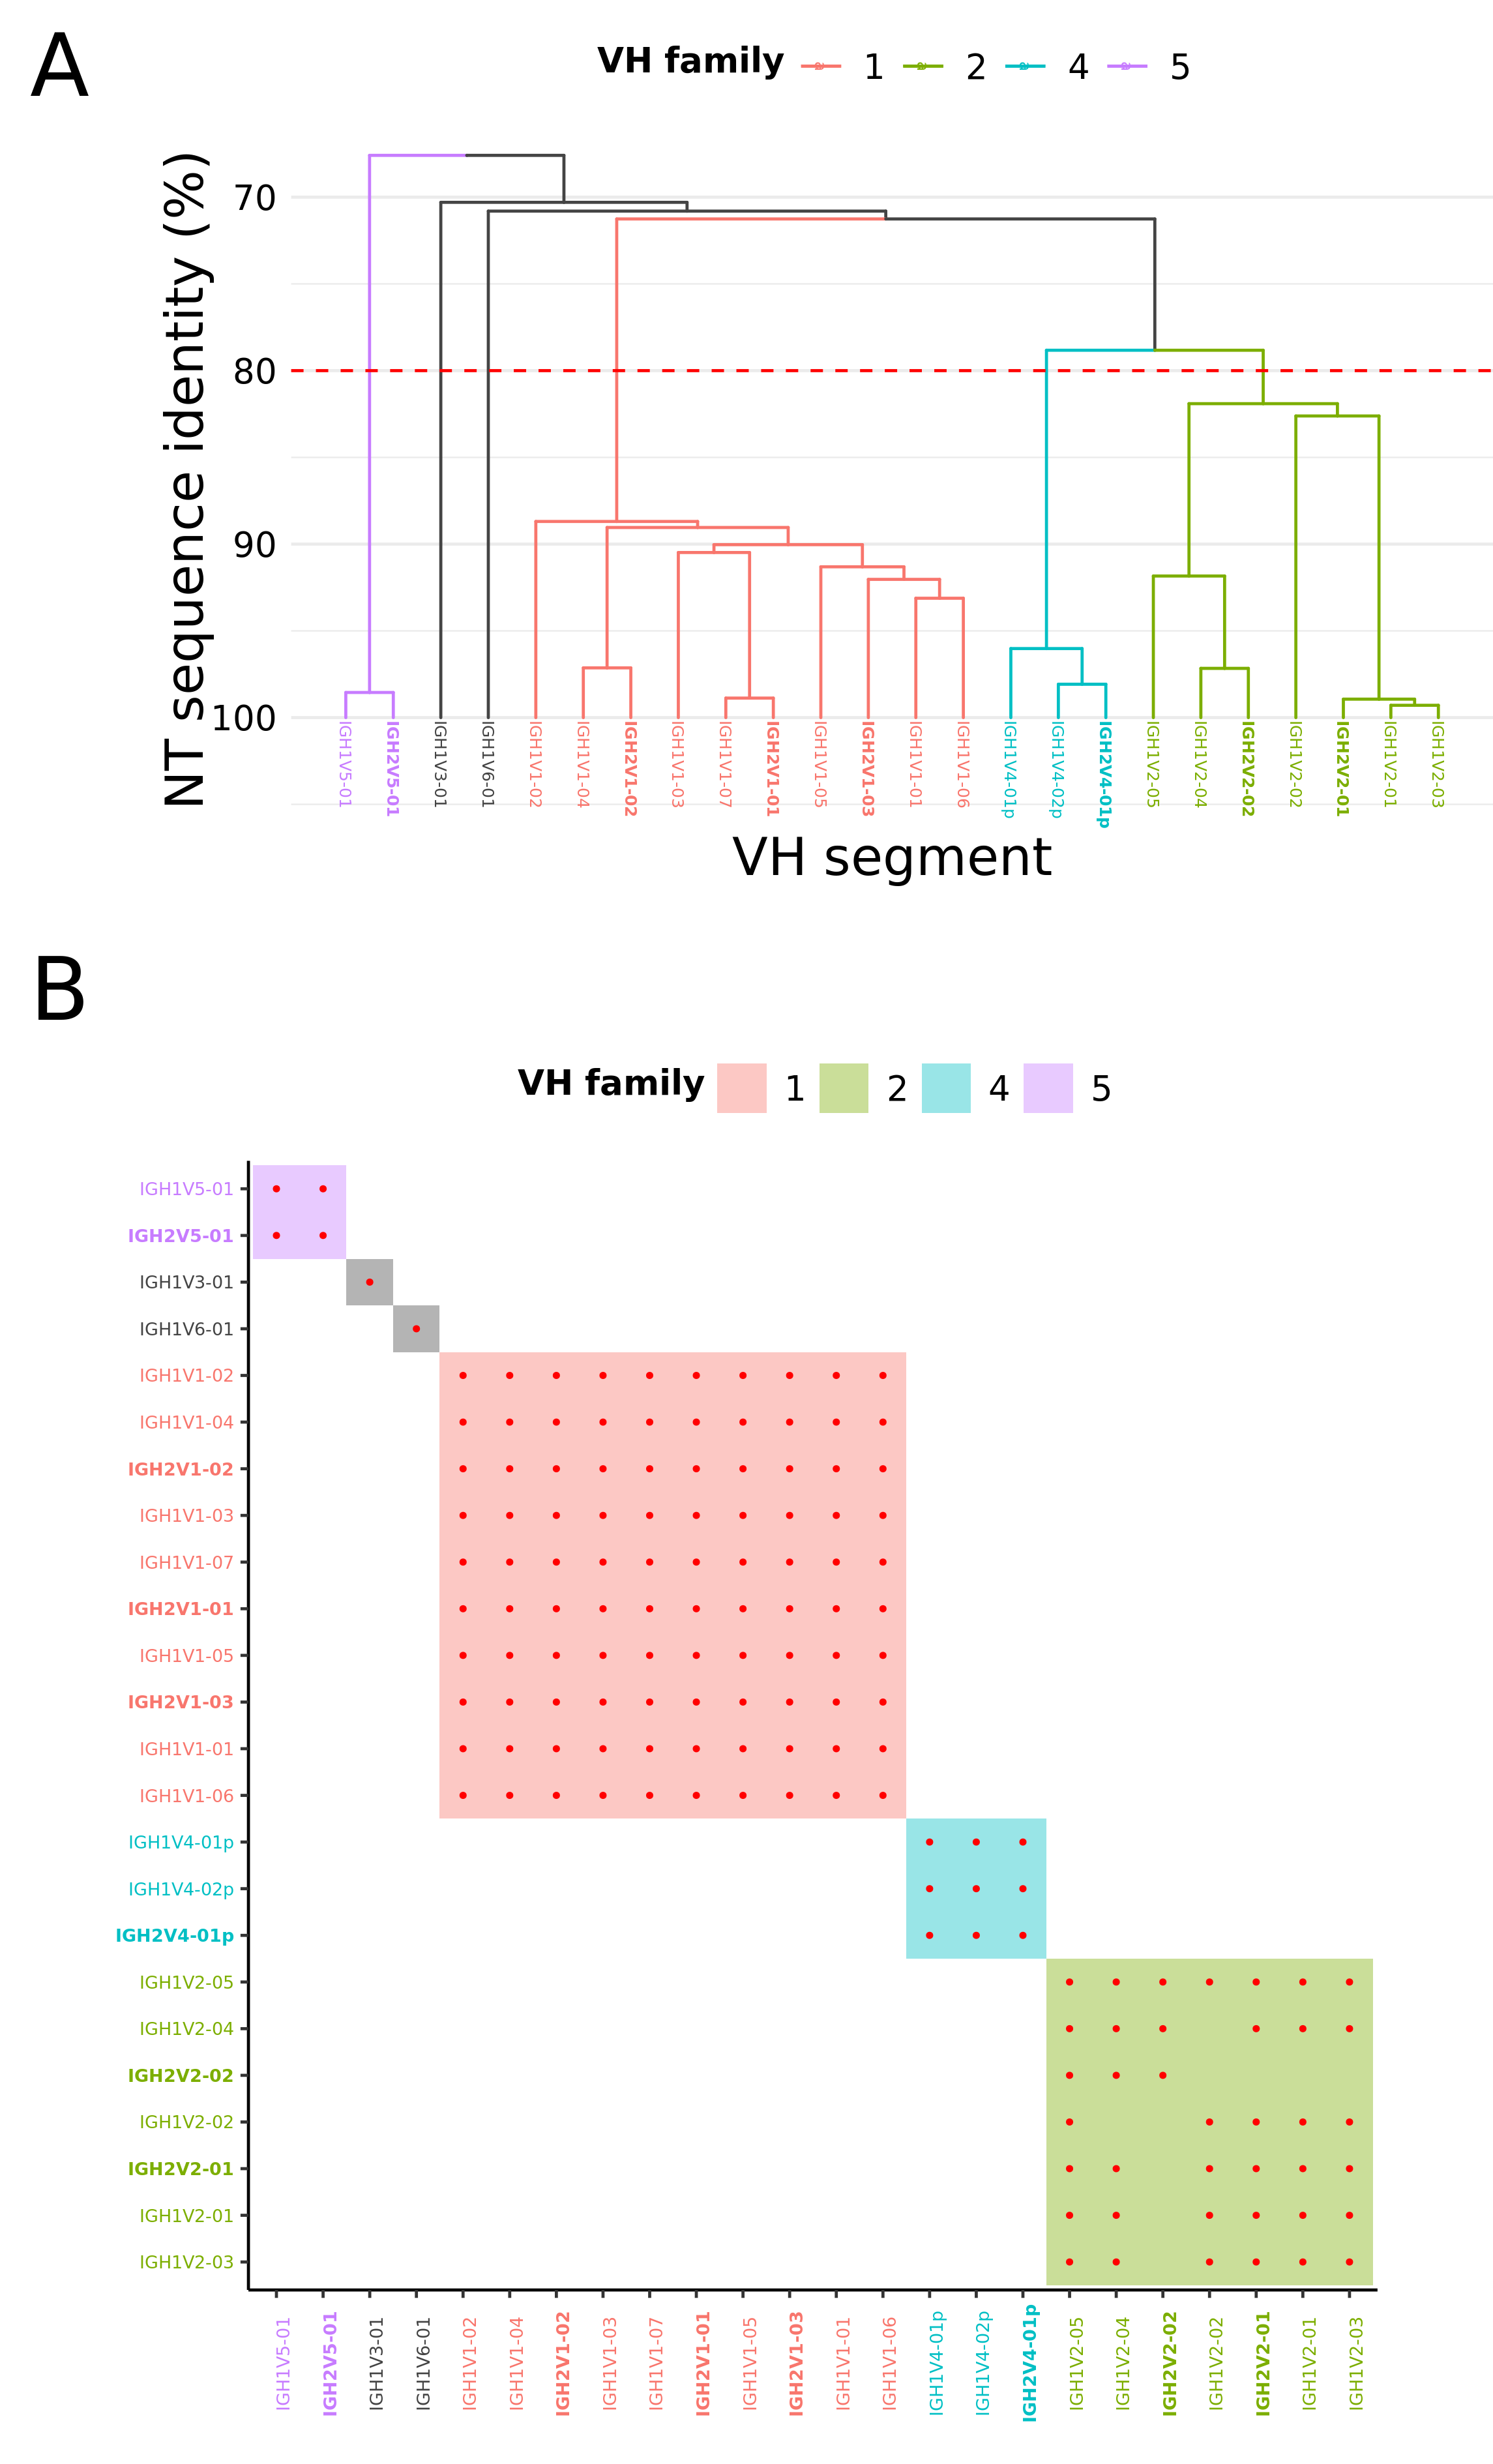
\includegraphics[width=0.8\textwidth]{_Figures/png/nfu-vh-families.png}
	\Caption{\vh families in the \Nfu \igh{} locus}{(A) Dendrogram of sequence similarity of \vh segments in the \Nfu \igh{} locus, arranged by single-linkage clustering on nucleotide sequence identity. The red line indicates the 80\,\% cutoff point for family assignment. (B) Heatmap of family relationships among \Nfu \vh segments, with shaded squares indicating families and red dots indicating pairwise nucleotide sequence identity of at least 80\,\%. In both subfigures, \vh families containing multiple segments are uniquely coloured, single-segment families are in grey, and segments from the \igh{2} sublocus are displayed in boldface.}
	\label{fig:nfu-vh-families}
	\end{figure}

\begin{figure}
\centering
	\centering
	\begin{subfigure}{0em}
	\phantomsubcaption{}
    \label{fig:nfu-dj-alignment-a}
    \end{subfigure}
    \begin{subfigure}{0em}
    \phantomsubcaption{}
    \label{fig:nfu-dj-alignment-b}
    \end{subfigure}
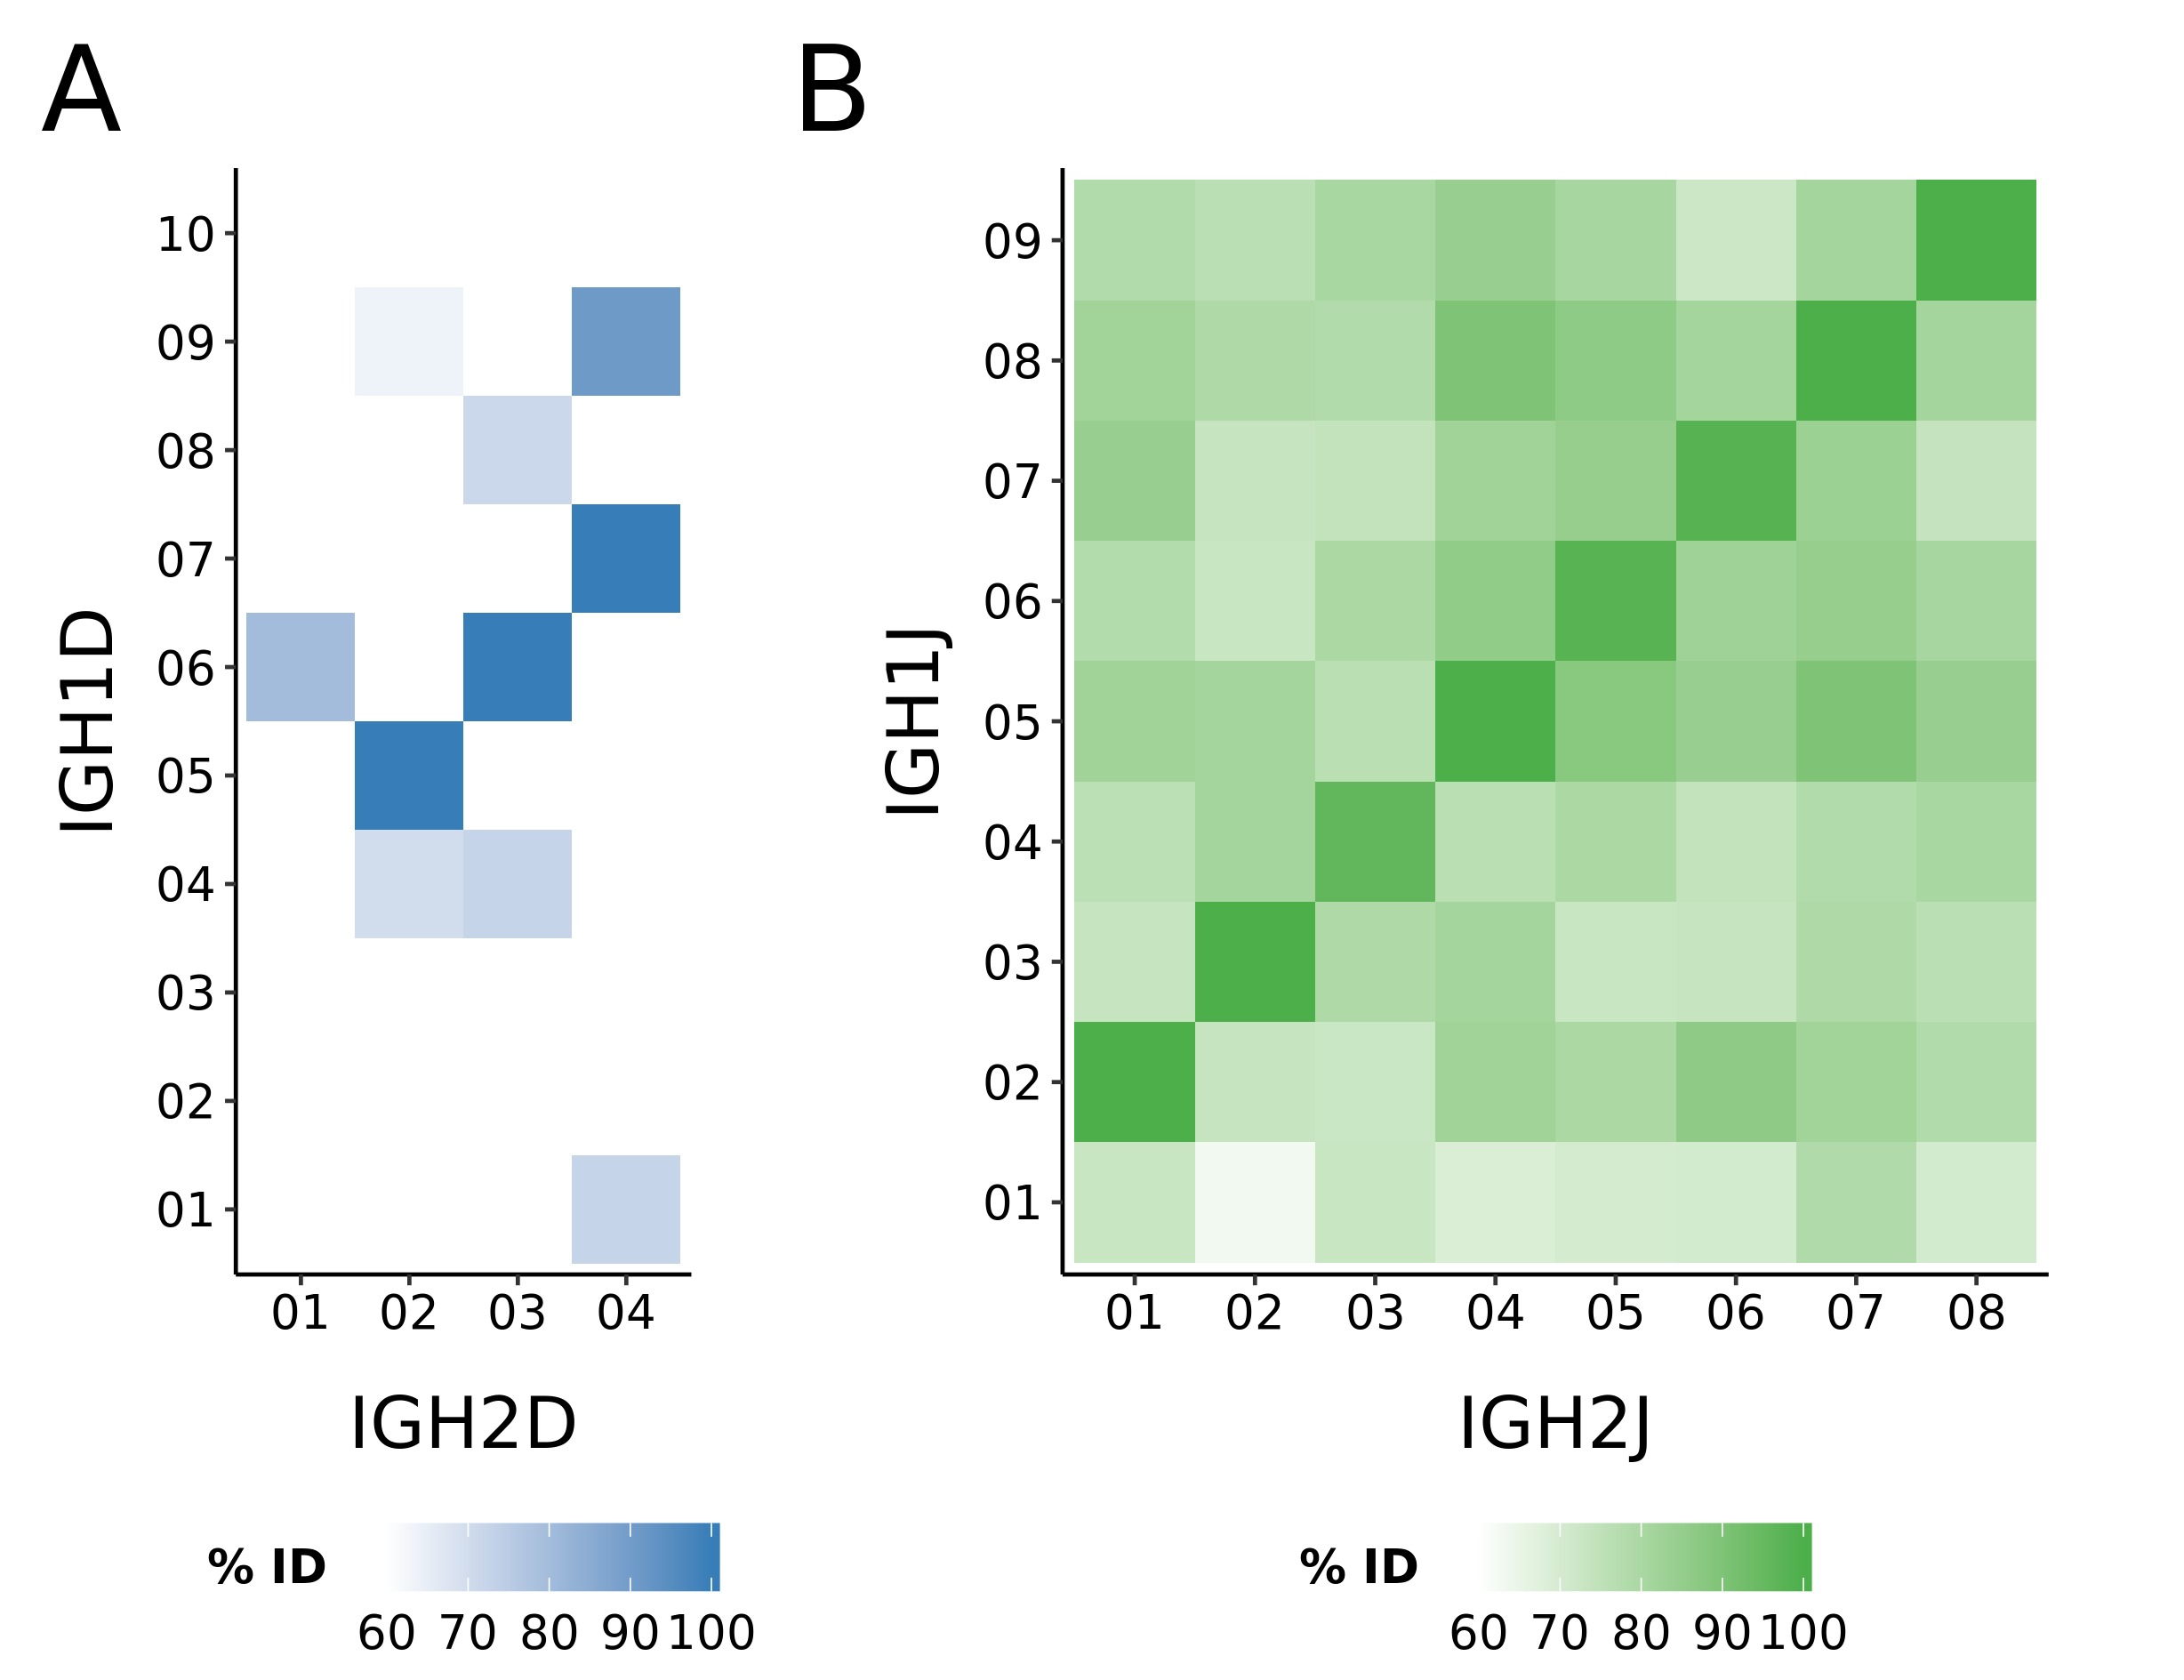
\includegraphics[width=0.6\textwidth]{_Figures/png/nfu-dj-aln}
\Caption{Cross-sublocus sequence similarity of \dh and \jh gene segments in \Nfu \igh{}}{Heatmap of percentage nucleotide sequence identities of Needleman-Wunsch global alignments between (A) \dh and (B) \jh gene segments in \igh{1} vs \igh{2}, revealing syntenic runs of highly similar sequences across both subloci.}
\label{fig:nfu-dj-alignment}
\end{figure}	
	
	\begin{figure}
	\centering
	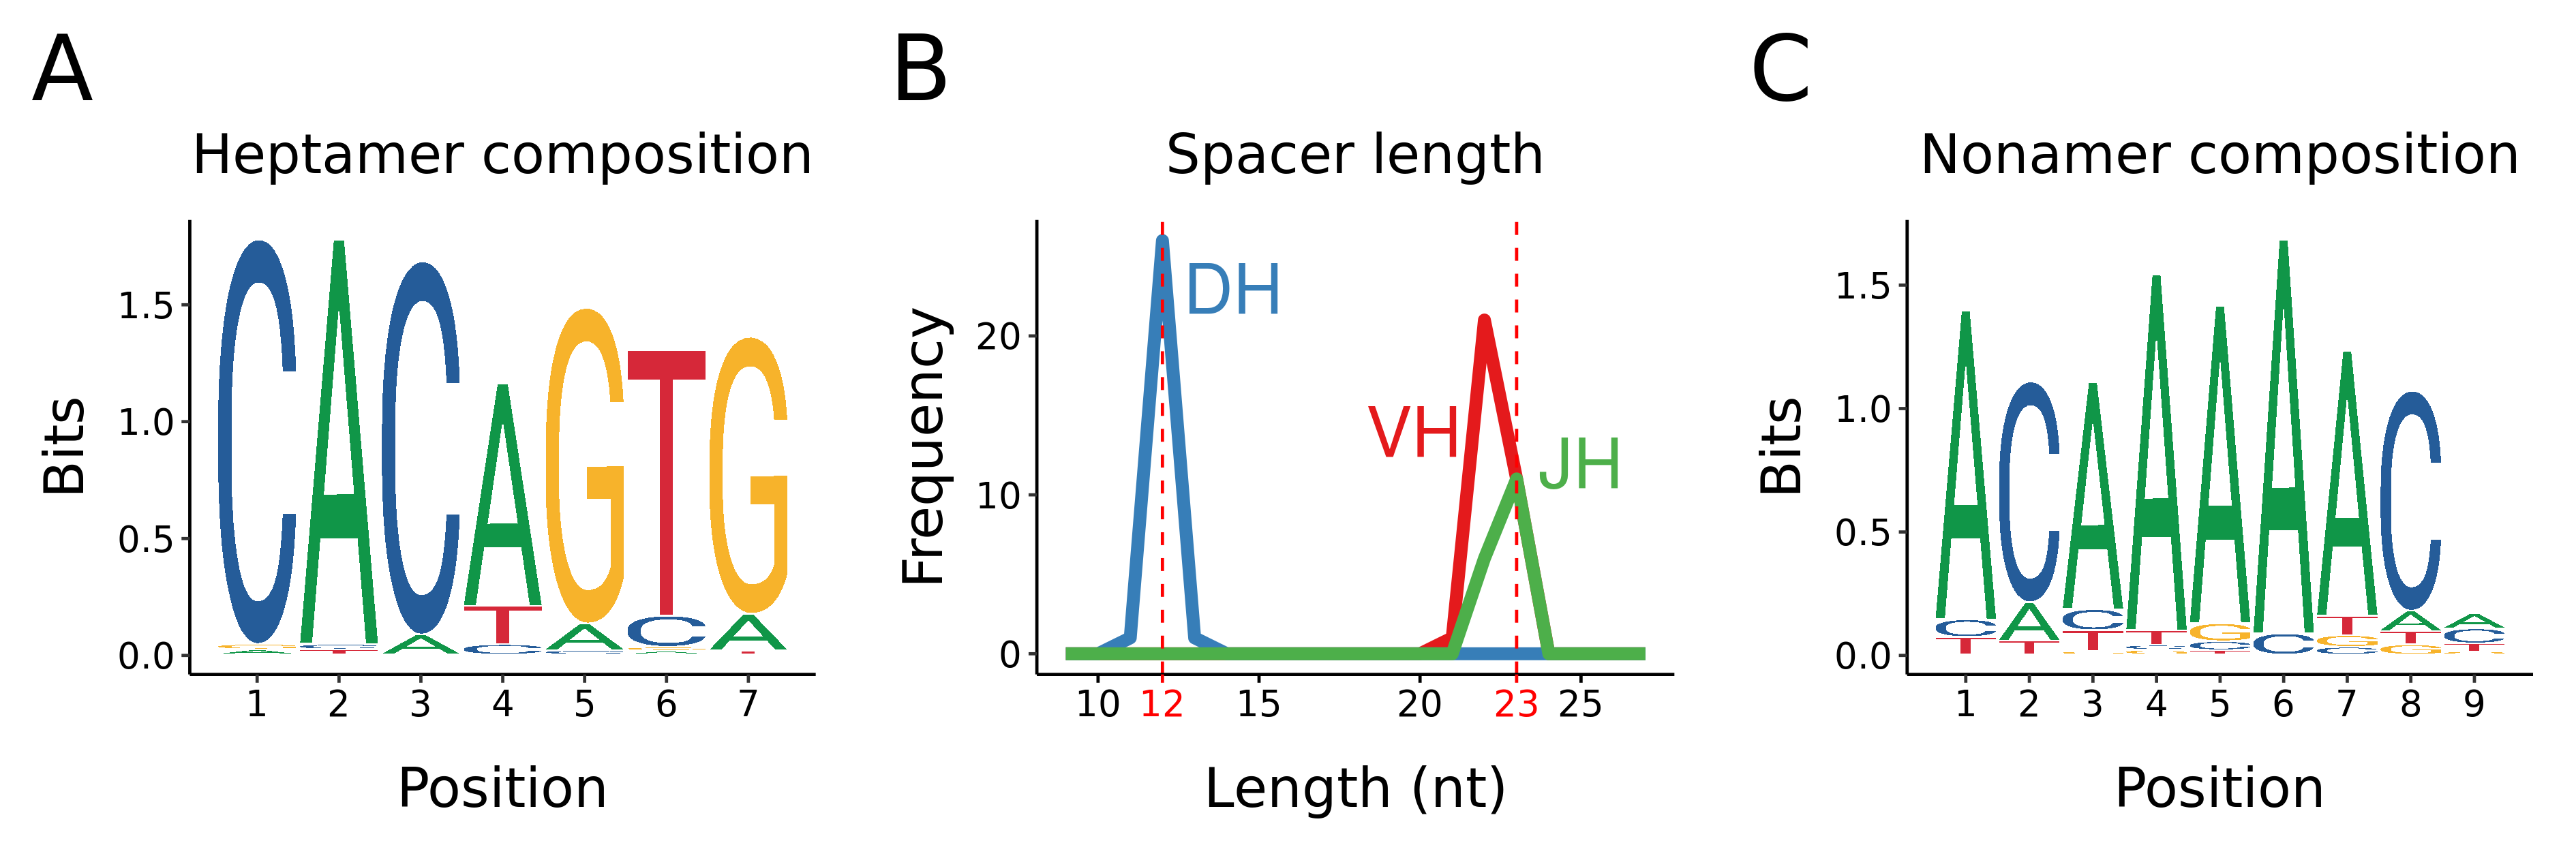
\includegraphics[width=\textwidth]{_Figures/png/nfu-rss-seqlogo-all}
	\Caption{Recombination signal sequences in \Nfu \igh{}}{(A) Sequence composition of conserved heptamer sequences across all \Nfu heavy-chain RSSs; (B) length distribution of unconserved spacer sequences in \Nfu heavy-chain RSSs; (C) sequence composition of conserved heptamer sequences across all \Nfu heavy-chain RSSs.}
	\label{fig:nfu-rss-seqlogo-all}
	\end{figure}
	
\FloatBarrier
\clearpage

\section{The \igh{} locus in \xma}
\label{sec:xma-locus}
	
	The turquoise-killifish \igh{} locus shares many features with other characterised teleost loci, including a modified tandem-translocon configuration with intact \vh, \dh, \jh and constant regions (\Cref{fig:nfu-locus-map-b}), a four-exon secreted configuration of \igh{M} (\Cref{fig:nfu-locus-sashimi-a}), an expanded \igh{D} constant region with tandem \cd{}-exon block repeats (\Cref{fig:nfu-locus-sashimi-b,fig:nfu-locus-map-b},), a conserved RSS structure (\Cref{fig:nfu-rss-seqlogo-all}), and a chimeric \cm{1} in \igh{D} (\Cref{fig:nfu-locus-sashimi-b}). However, it also exhibits many ideosyncratic features that differ from those observed in most characterised teleost loci, including an unusually small number of \vh segments (\Cref{fig:nfu-vh-families} and \Cref{tab:teleost-vh-counts}), a four-exon \cm{1}-\cm{2}-TM1-TM2 configuration of transmembrane \igh{M} (\Cref{fig:nfu-locus-sashimi-a}), an inverted sublocus present in antisense (\Cref{fig:nfu-locus-map-b}), and a complete absence of \igh{Z}.
	
Many of these peculiarities, including the unusual \igh{M-TM} splicing pattern, inverted sublocus, and lack of \igh{Z}, are shared with the \igh{} locus of medaka (\textit{Oryzias latipes}), which is the closest relative of \textit{Nothobranchius furzeri} to have its immunoglobulin heavy chain locus characterised prior to this study \parencite{magadan2011medaka}. Given the close relationship between the two species, the shared unusual features of their \igh{} loci suggested a common origin of these traits  in the common ancestor of both species. If this hypothesis were correct, one would expect \igh{Z} to also be absent in any other descendents of this common ancestor, including other cyprinodontiform species.

To investigate this hypothesis further, I performed a complete characterisation of the \igh{} locus in the platyfish \textit{Xiphophorus maculatus}, another cyprinodontiform species that has seen widespread use as a model organism \parencite{schartl2013platyfish}. Surprisingly, the \Xma locus possessed none of the unusual features shared between the turquoise-killifish and medaka loci, strongly suggesting independent loss of \igh{Z} in \Nfu and medaka and implying a high level of volatility in \igh{} locus structure in this group of teleost fishes.

\subsection{Overall structure}
\label{sec:xma-locus-structure}
	
As was the case with the \Nfu \igh{} locus, I identified candidate genome scaffolds from the most recent \xma genome assembly (Genbank accession GCA\_002775205.2) by aligning them to \igh{} gene segments from zebrafish, stickleback and medaka, supplemented in this case with segments from the newly-characterised \Nfu locus itself. In contrast to the more fragmented results in \Nfu, this process identified a single sequence region on one chromosome of the \Xma locus, which I extracted and characterised as described for the assembled \Nfu locus (\Cref{sec:nfu-locus}) without the need for further sequencing or assembly.

The \Xma \igh{} locus so identified occupies roughly \kb{293} on chromosome 16 (scaffold NC\_036458.1; \Cref{fig:xma-locus-map-a}). Unlike in turquoise killifish and medaka, all identified gene segments share a common orientation; no evidence of a second sublocus in antisense could be identified. In stark contrast with both turquoise killifish and medaka, the single ``sublocus'' comprising \Xma \igh{} contains not one but two \igh{Z} constant regions, along with a hugely extended V-region extending over almost \kb{250} and containing more than 120 \vh-segments (\Cref{fig:xma-locus-map-b}). This enormous \vh-diversity exceeds that of almost all previously-characterised teleost \igh{} loci (\Cref{sec:intro_teleost_loci}), while the presence of multiple \igh{Z} constant regions without intervening \igh{M} or \igh{D} is also highly unusual \parencite{fillatreau2013astonishing}. 

Even cursory examination of the \Xma \igh{} locus is therefore sufficient to reveal a unique and highly interesting structure with many unexpected differences from both turquoise killifish and medaka (\Cref{fig:species-tree-small}, columns 1-5). In particular, since \Xma is more closely related to \Nfu than either is to medaka, the presence of \igh{Z} in the former strongly suggests at least two independent loss events in the lineage containing turquoise killifish and medaka, indicating an unexpected level of volatility in the evolution of this important isotype.
 
	\begin{figure}
	\centering
	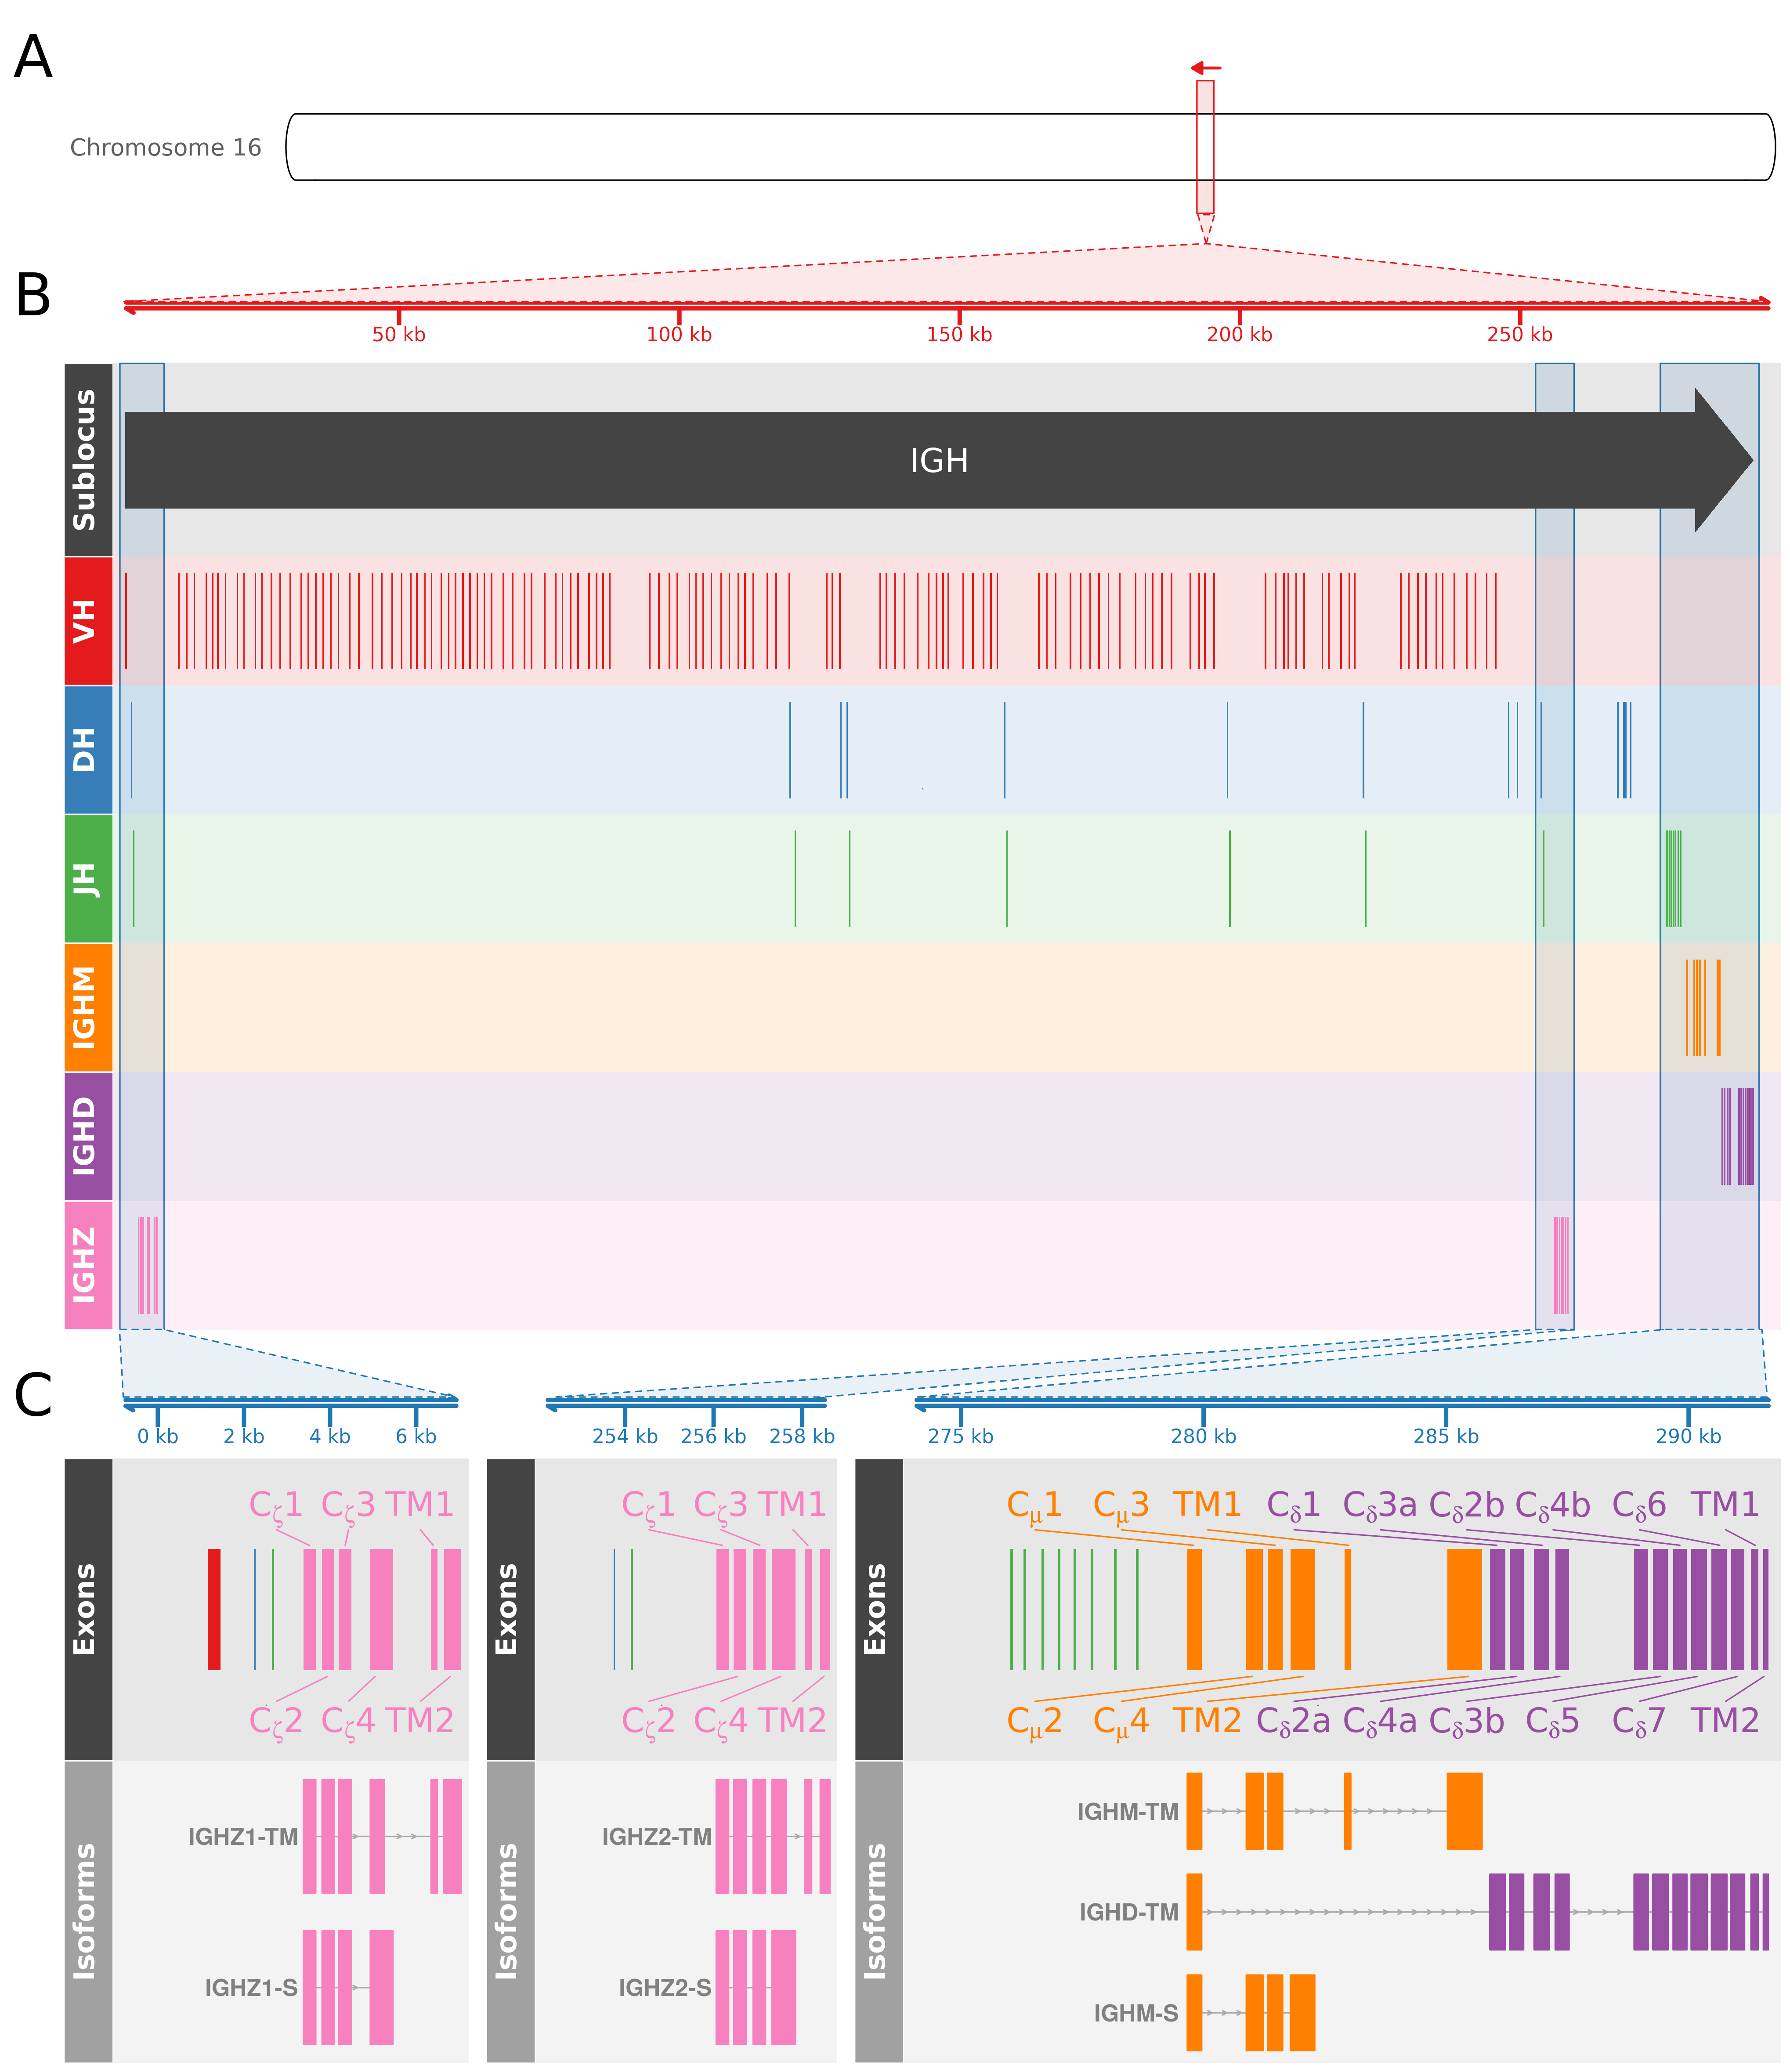
\includegraphics[width=\textwidth]{_Figures/png/xma-new-locus-map}
	\Caption{The immunoglobulin heavy chain (\igh{}) locus in \xma}{(A) Position of the \igh{} locus on chromosome (group) 16 of the \Xma genome. (B) Arrangement of \vh, \dh, \jh and constant-region gene segments on the \Xma \igh{} locus. (C) Detailed map of the \igh{Z1}, \igh{Z2} and \igh{M/D} constant regions, indicating the position and identity of the constant-region exons and the exon composition of expressed \igh{} isoforms in \Xma. Note change of orientation between subfigures (A) and (B-C).}
	\begin{subfigure}{0em}
        \phantomsubcaption{}
        \label{fig:xma-locus-map-a}
    \end{subfigure}
    \begin{subfigure}{0em}
        \phantomsubcaption{}
        \label{fig:xma-locus-map-b}
    \end{subfigure}
    \begin{subfigure}{0em}
        \phantomsubcaption{}
        \label{fig:xma-locus-map-c}
    \end{subfigure}
	\label{fig:xma-locus-map}
\end{figure}

\begin{figure}
\centering
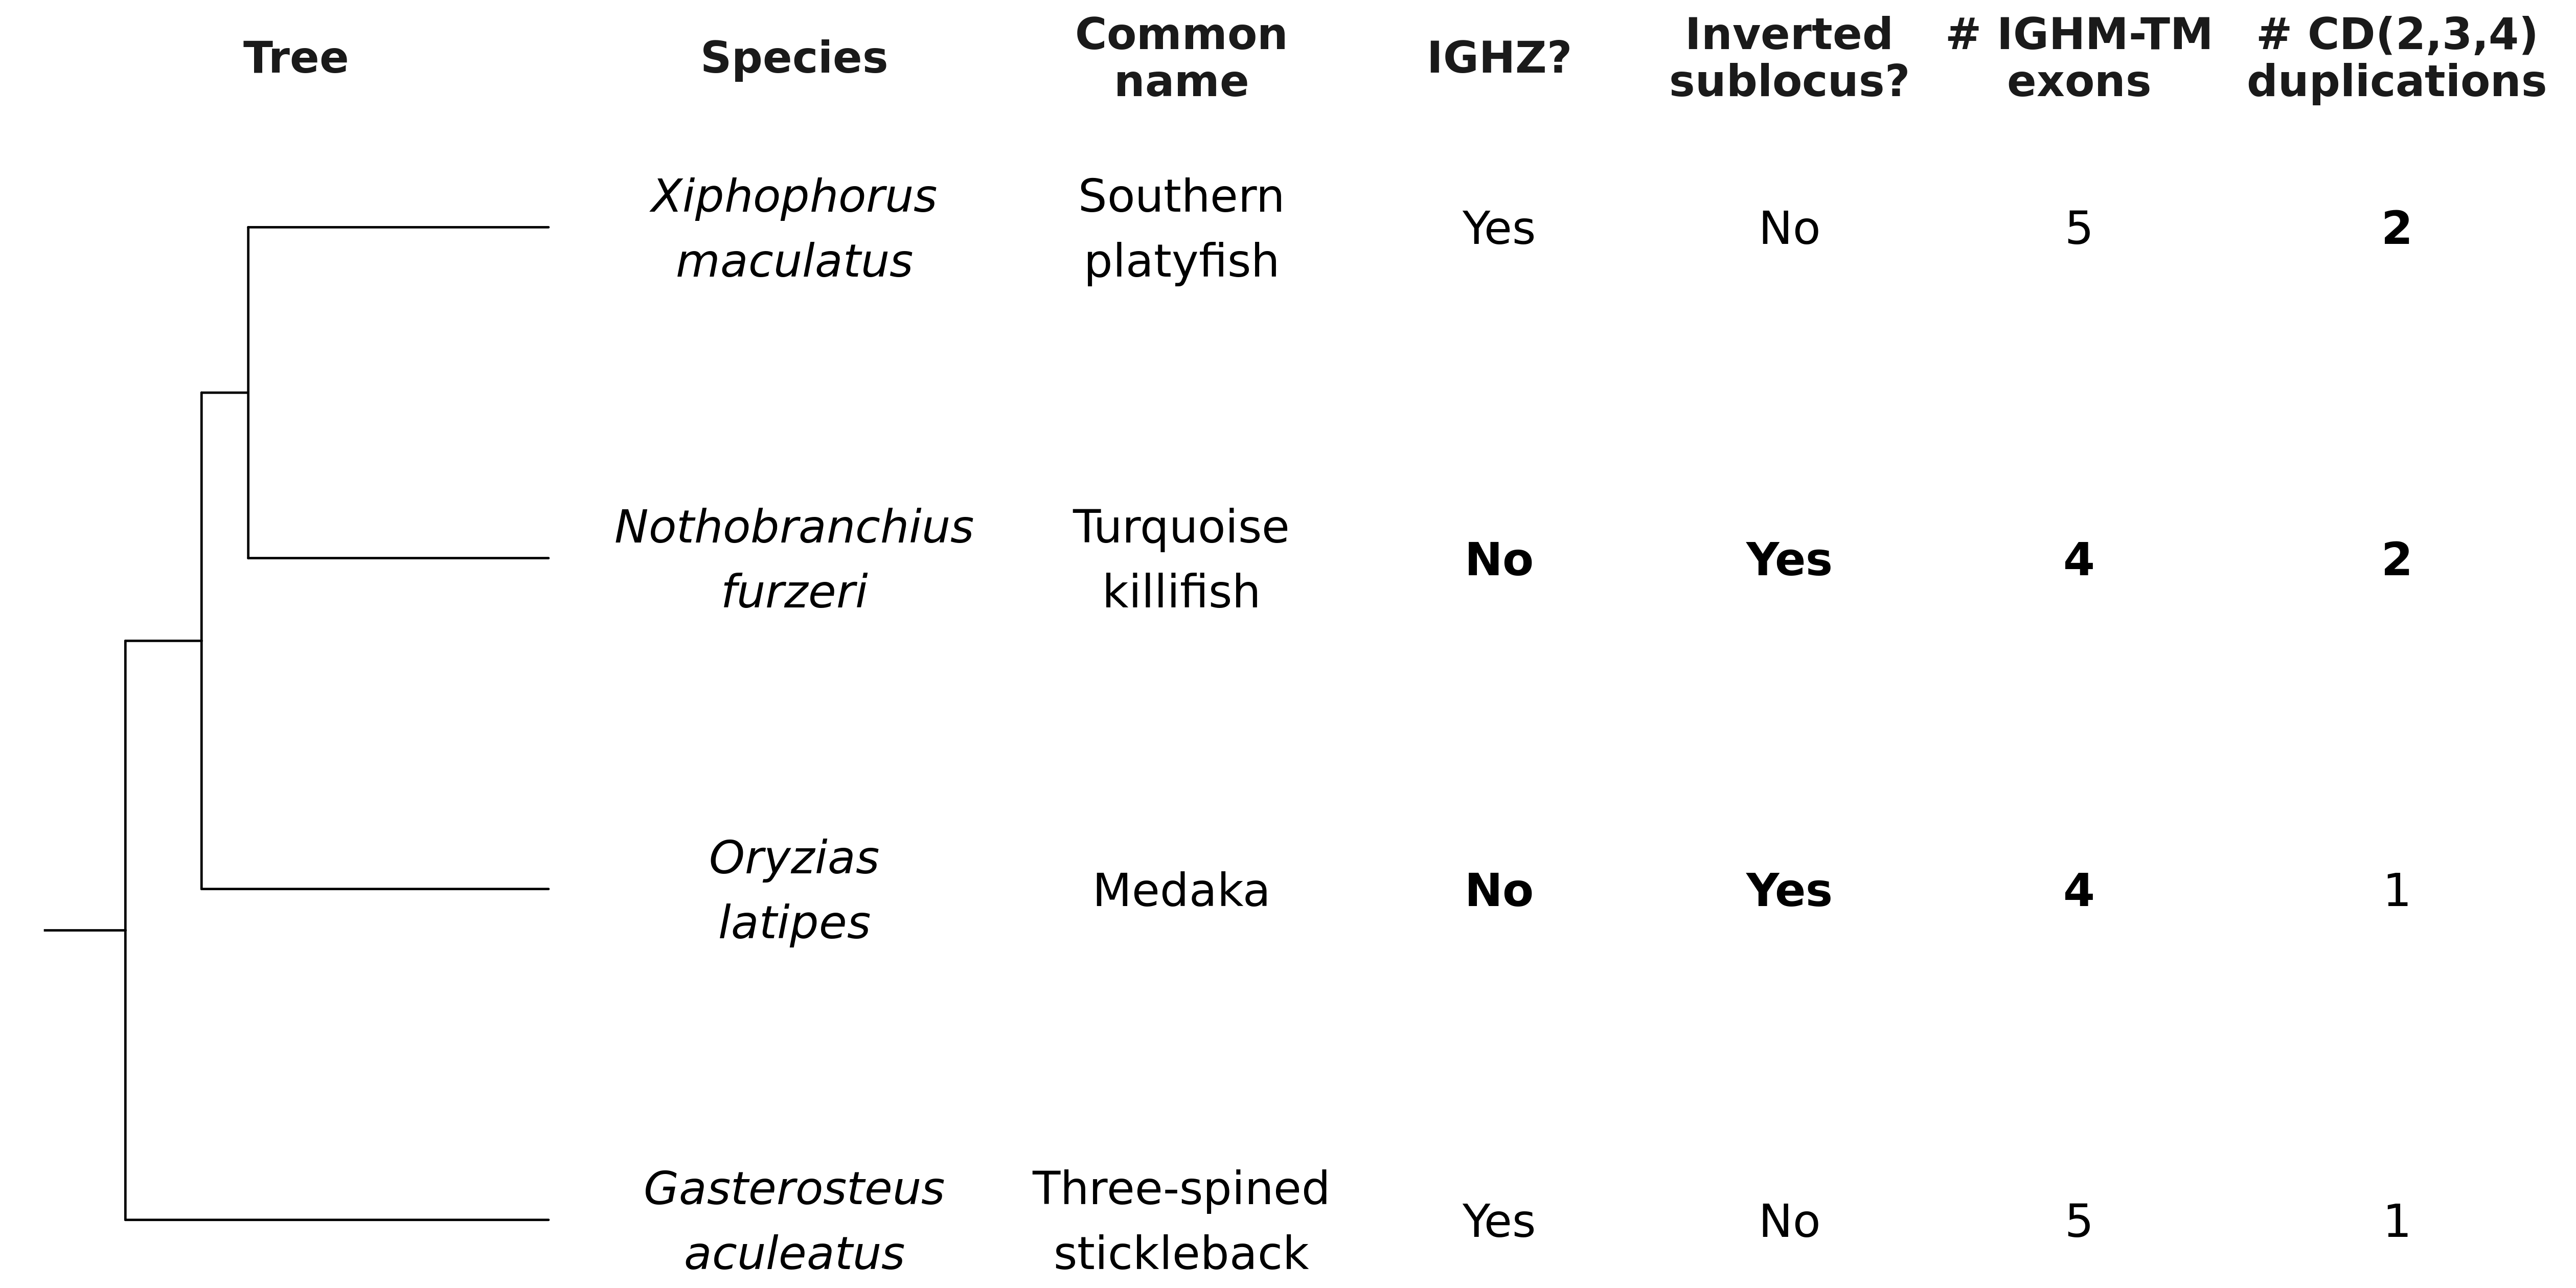
\includegraphics[width=\textwidth]{_Figures/png/species-tree-small}
\vspace{0.5em}
\Caption{Important \igh{} phenotypes in turquoise killifish, southern platyfish, and medaka}{Cladogram of the evolutionary relationship between southern platyfish (\xma), turquoise killifish (\nfu) and medaka (\species{Oryzias}{latipes}), with three-spined stickleback (\species{Gasterosteus}{aculeatus}) as an outgroup. The state of various \igh{} phenotypes of interest are annotated to the right of the tree; states deviating from the expected teleost configuration are in bold.}
\label{fig:species-tree-small}
\end{figure}
	
\subsection{Constant regions}
\label{sec:xma-locus-constant}
	
As discussed briefly in \Cref{sec:xma-locus-structure}, the \Xma \igh{} locus contains two distinct \igh{Z} constant regions: one in the usual position immediately preceding the \igh{M}-associated D- and J-regions, the other, unexpectedly, at the far 5'-extremity of the locus (\Cref{fig:xma-locus-map-b}). Both \igh{Z} constant regions occupy the expected configuration, with four \cz{} exons, two transmembrane exons, and a secretory tail (\Cref{fig:xma-locus-map-c}, \Cref{tab:xma-ch-coords}). However, in contrast to the duplicate constant regions in \Nfu, the two \igh{Z} constant regions in \Xma are quite distinct from each other in sequence, with an average of only \pc{64} nucleotide and \pc{48} amino-acid sequence identity between corresponding \cz{} exons (\Cref{fig:xma-cz-aln}, \Cref{tab:xma-cz-aln}). This unexpectedly high level of sequence divergence suggests a relatively ancient duplication event, and raises the possibility that the lineage giving rise to \Nfu may have lost not one, but two distinct \igh{Z} constant regions.
	
\begin{table}
	\centering
	\Caption{Sequence similarity between \igh{Z} constant-regions in \Xma}{Percentage sequence identities of pairwise Needleman-Wunsch global alignments between nucleotide (NT) or amino-acid (AA) sequences of corresponding \cz{} exons from the two \igh{Z} constant regions of \Xma \igh{}.}
	% latex table generated in R 3.5.2 by xtable 1.8-3 package
% Tue Jan  8 14:15:22 2019
\begin{tabular}{llrr}
  \toprule Isotype & Exon & NT & AA \\ 
  \midrule Z & 1 & 59.14 & 44.57 \\ 
  Z & 2 & 63.93 & 53.41 \\ 
  Z & 3 & 66.19 & 43.48 \\ 
  Z & 4 & 65.15 & 50.49 \\ 
   \bottomrule \end{tabular}

	\label{tab:xma-cz-aln}
\end{table}

While the state of \igh{Z} constant regions differs markedly between \Xma and \Nfu, the configurations of the \igh{M} and \igh{D} constant regions of the two species are quite similar, with a {\cm{1}-\cm{2}-\cm{3}-\cm{4}-TM1-TM2} configuration for \igh{M} and a {\cd{1}-(\cd{2}-\cd{3}-\cd{4})$_2$-\cd{5}-\cd{6}-\cd{7}-TM1-TM2} configuration for \igh{D} (\Cref{fig:xma-locus-map-b,fig:xma-locus-map-c}, \Cref{tab:xma-ch-coords}). In the \Xma locus, these constant regions and \igh{Z2} adopt the standard configuration seen in comparatively simple teleost \igh{} loci like those of zebrafish and fugu, with a {\vh-\dh-\jh-\textbf{CZ}-\dh-\jh-\textbf{CM}-\textbf{CD}} arrangement that allows the choice between \igh{Z} and \igh{M/D} usage to be made via the choice of \dh segment during VDJ-recombination. However, whether such a mechanism is also responsible for the choice between these constant regions and \igh{Z1}, which lies more than \kb{200} away and upstream of the great majority of \vh segments in the locus (\Cref{sec:xma-locus-variable}) is questionable.

In order to investigate the expressed isoforms present in \Xma, I aligned published RNA-sequencing reads from various platyfish tissues (BioProject accession PRJNA420092, all libraries, \Cref{tab:rnaseq-sources}) to the \igh{Z} and \igh{M/D} constant regions with \program{STAR}. The results indicate the expected six-exon transmembrane configuration in both \igh{Z1} and \igh{Z2}, as well as a secretory form of \igh{Z1} comprising \cz{1} to \cz{4} plus a \bp{23} secretory tail formed by a transcriptional run-on event from \cz{4} (\Cref{fig:xma-locus-sashimi-z1,fig:xma-locus-sashimi-z2}). However, while an in-frame secretory tail of similar length (\bp{20}) can be found in \igh{Z2}, it does not appear to be expressed in the read sets analysed here, suggesting that \igh{Z2} may only be expressed in transmembrane form in the individuals sampled (\Cref{fig:xma-locus-sashimi-z2}).

Meanwhile, the results for \igh{D} (\Cref{fig:xma-locus-sashimi-d}) indicate a similar configuration to that observed in turquoise killifish, with a chimeric \cm{1} followed by 10 \cd{} exons and two transmembrane exons; as in \Nfu, neither a dedicated \igh{D} secretory exon nor a post-\cd{7} secretory tail was identified, suggesting that \igh{D} may be produced solely in transmembrane form in \Xma. Secretory \igh{M} (\igh{M-S}) was also found to occupy the same four-exon configuration seen in turquoise killifish and elsewhere. However, the configuration observed for transmembrane \igh{M} (\igh{M-TM}) did not correspond to the four-exon structure shared between turquoise killifish and medaka (\Cref{fig:xma-locus-sashimi-m,fig:nfu-locus-sashimi-a}); rather, \igh{M-TM} in \Xma occupies the five-exon configuration seen in most characterised teleosts (\Cref{fig:teleost-igm-exons-d}). This surprising difference indicates that two different splice configurations of \igh{M-TM} persist in the cyprinodontiform lineage, and raises the question of what, if any, functional difference arises from the presence or absence of \cm{3} in transmembrane \igh{M} in different species. However, it remains unclear whether this pattern of exon usage (\Cref{fig:species-tree-small}) is the result of independent changes in medaka and turquoise killifish or of a reversion in \Xma to the primitive teleost configuration.
	
\begin{figure}
	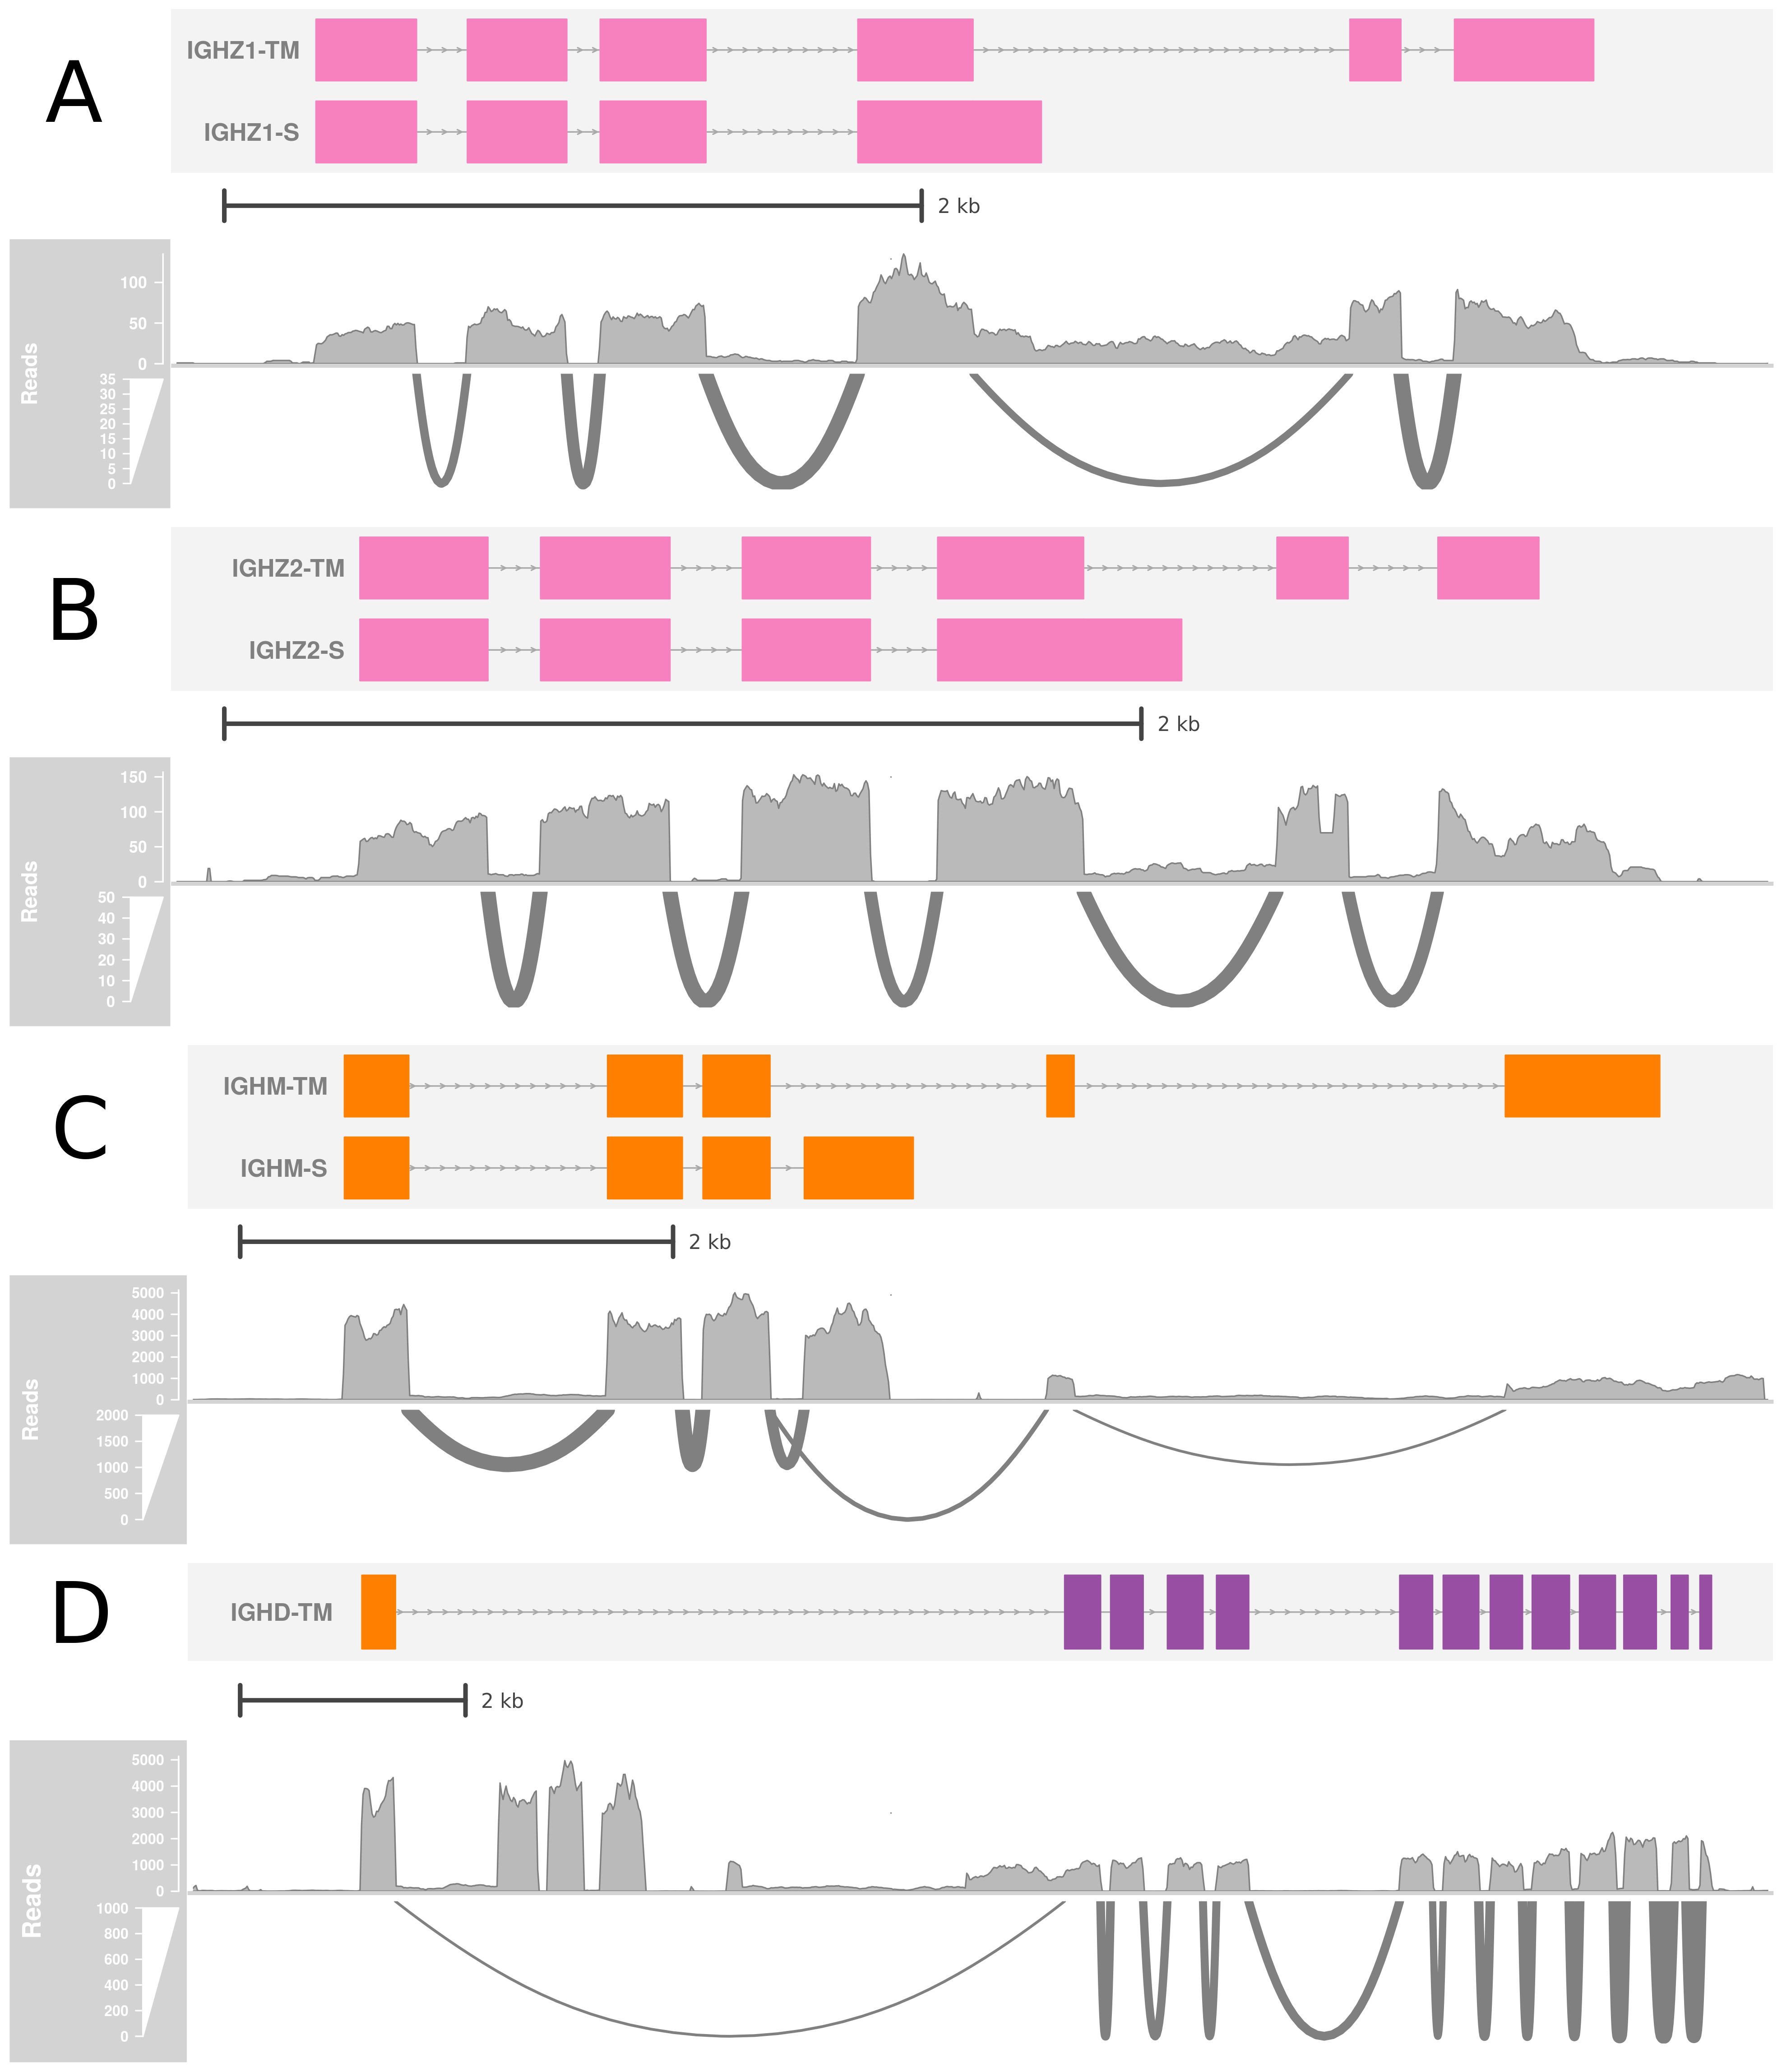
\includegraphics[width=\textwidth]{_Figures/png/xma-new-locus-sashimi}
	    \begin{subfigure}{0em}
        \phantomsubcaption{}
        \label{fig:xma-locus-sashimi-z1}
    \end{subfigure}
    \begin{subfigure}{0em}
        \phantomsubcaption{}
        \label{fig:xma-locus-sashimi-z2}
    \end{subfigure}
	\begin{subfigure}{0em}
        \phantomsubcaption{}
        \label{fig:xma-locus-sashimi-m}
    \end{subfigure}
    \begin{subfigure}{0em}
        \phantomsubcaption{}
        \label{fig:xma-locus-sashimi-d}
    \end{subfigure}
	\Caption{Constant-region isoforms in \Xma}{Coverage and Sashimi plots \parencite{katz2013sashimi} of STAR-aligned RNA-seq reads from \Xma samples, demonstrating the splicing behaviour of \igh{} constant-region isoforms and showing the read coverage of each exon and splice junction. (A) \igh{Z1} exon splicing, showing alternative use of the \cz{4}/TM1 splice junction and the post-\cz{4} secretory tail; (B) \igh{Z2} exon splicing, showing the apparent lack of expression of the \igh{Z2} secretory isoform; (C) \igh{M} exon splicing, showing alternative splicing patterns of \igh{M-TM} and \igh{M-S}; (D) \igh{D} exon splicing, showing chimeric splicing of \cm{1} to \cd{1}.}
	\label{fig:xma-locus-sashimi}
	\end{figure}

	
\subsection{Variable regions}
\label{sec:xma-locus-variable}

In total, I identified 125 \vh segments, 14 \dh segments and 15 \jh segments in the \Xma \igh{} locus (\Cref{fig:xma-locus-map-b}). Of these, exactly one \vh (\igh{V01-01}), \dh (\igh{DZ01}) and \jh (\igh{JZ01}) lie upstream of the \igh{Z1} constant region, indicating that the variable-region sequence diversity available to this isotype is limited to a single VDJ combination. In contrast, the variable region between the end of \igh{Z1} and the start of \igh{Z2} is highly expanded, with 124 tightly-clustered \vh segments -- more than five times the total number seen in \Nfu, and more than seven times the number in the largest \Nfu sublocus. Of these 124 \vh segments, 106 (\pc{86}) are apparently functional, with the remainder pseudogenised by a variety of frameshift mutations, nonsense mutations, or truncation events (\Cref{tab:xma-vh-coords-1,tab:xma-vh-coords-2,tab:xma-vh-coords-3,tab:xma-vh-coords-4,tab:xma-vh-coords-5}); it remains to be seen whether \igh{V01-01} is also capable of recombining with \dh segments downstream of the \igh{Z1} constant region, and so constitutes part of the range of VDJ combinations available to the other constant regions. The \vh sequences in the \Xma locus are much more tightly packed than in the \Nfu locus, consistent with a lower overall prevalence of repetitive regions (21\,\%) in the \Xma genome \parencite{yuan2018repeats}.
	
In total, the \vh regions in \Xma \igh{} fall into 23 families, of which eight contain multiple segments (\Cref{fig:xma-vh-families-tree,fig:xma-vh-families-map}); strikingly, the single \vh segment serving \igh{Z} (\igh{V01-01}) represents a separate family which is distinct from any other segment in the locus. To further investigate the evolutionary history of these families, I aligned the \vh segments from both the \Xma and \Nfu \igh{} loci together with \program{PRANK}, and used the resulting alignment to construct a phylogenetic tree with \program{RAxML} \parencite{stamatakis2014raxml8,stamatakis2005raxml3,stamatakis2006raxml6}; the resulting tree (\Cref{fig:nfu-xma-vh-tree-nt}) revealed a clear interrelationship between the largest families in both loci (\Xma V02 and \Nfu V1), with a similar relationship observed for the second-largest families (\Xma V03 and \Nfu V2). 
In accordance with the close sequence relationship noted in \Cref{sec:nfu-locus-variable}, \Nfu V4 falls comfortably within the V03/V2 subtree, supporting its status as a pseudogenised subfamily of \Nfu V2.
		
In addition to its highly expanded \vh region, the variable region of the \Xma locus is unusual in the arrangement of its \dh and \jh segments (\Cref{tab:xma-dh-coords-seg,tab:xma-jh-coords-seg}): in addition to the relatively densely-packed blocks of four \dh and eight \jh segments between \igh{Z2} and \igh{M}, and the smaller groups of three \dh segments and one \jh segment between the last \vh segment and \igh{Z2}, small numbers of \dh and \jh segments are interspersed between blocks of \vh segments in the extended V-region between \igh{Z1} and \igh{Z2} (\Cref{fig:xma-locus-map-b}). Many of these segments are arranged such that groups of one or two \dh segments are closely associated with a single \jh segment, raising the possibility of a more cluster-like behaviour in which each VDJ block acts as a distinct recombination unit. However, the presence of larger D- and J-regions more closely upstream of the constant regions suggests a more conventional translocon behaviour; it remains to be seen which of these traditional models of antigen-receptor structure more closely matches the \textit{in vivo} recombination behaviour of this locus.
		
Finally, as is the case with \Nfu, the recombination signal sequences (RSSs) in \Xma \igh{} correspond closely to the standard expectations across the vertebrates, with the expected heptamer and nonamer consensus sequences and spacer length distributions (\Cref{fig:xma-rss-seqlogo-all,fig:xma-rss-seqlogo-sep}, 97.6\,\% of RSS spacers within \bp{1} of the expected conserved length).	

	\begin{figure}
		\begin{subfigure}{0em}
        \phantomsubcaption{}
        \label{fig:xma-rss-seqlogo-all-heptamer}
    \end{subfigure}
    \begin{subfigure}{0em}
        \phantomsubcaption{}
        \label{fig:xma-rss-seqlogo-all-spacer}
    \end{subfigure}
    \begin{subfigure}{0em}
        \phantomsubcaption{}
        \label{fig:xma-rss-seqlogo-all-nonamer}
    \end{subfigure}
	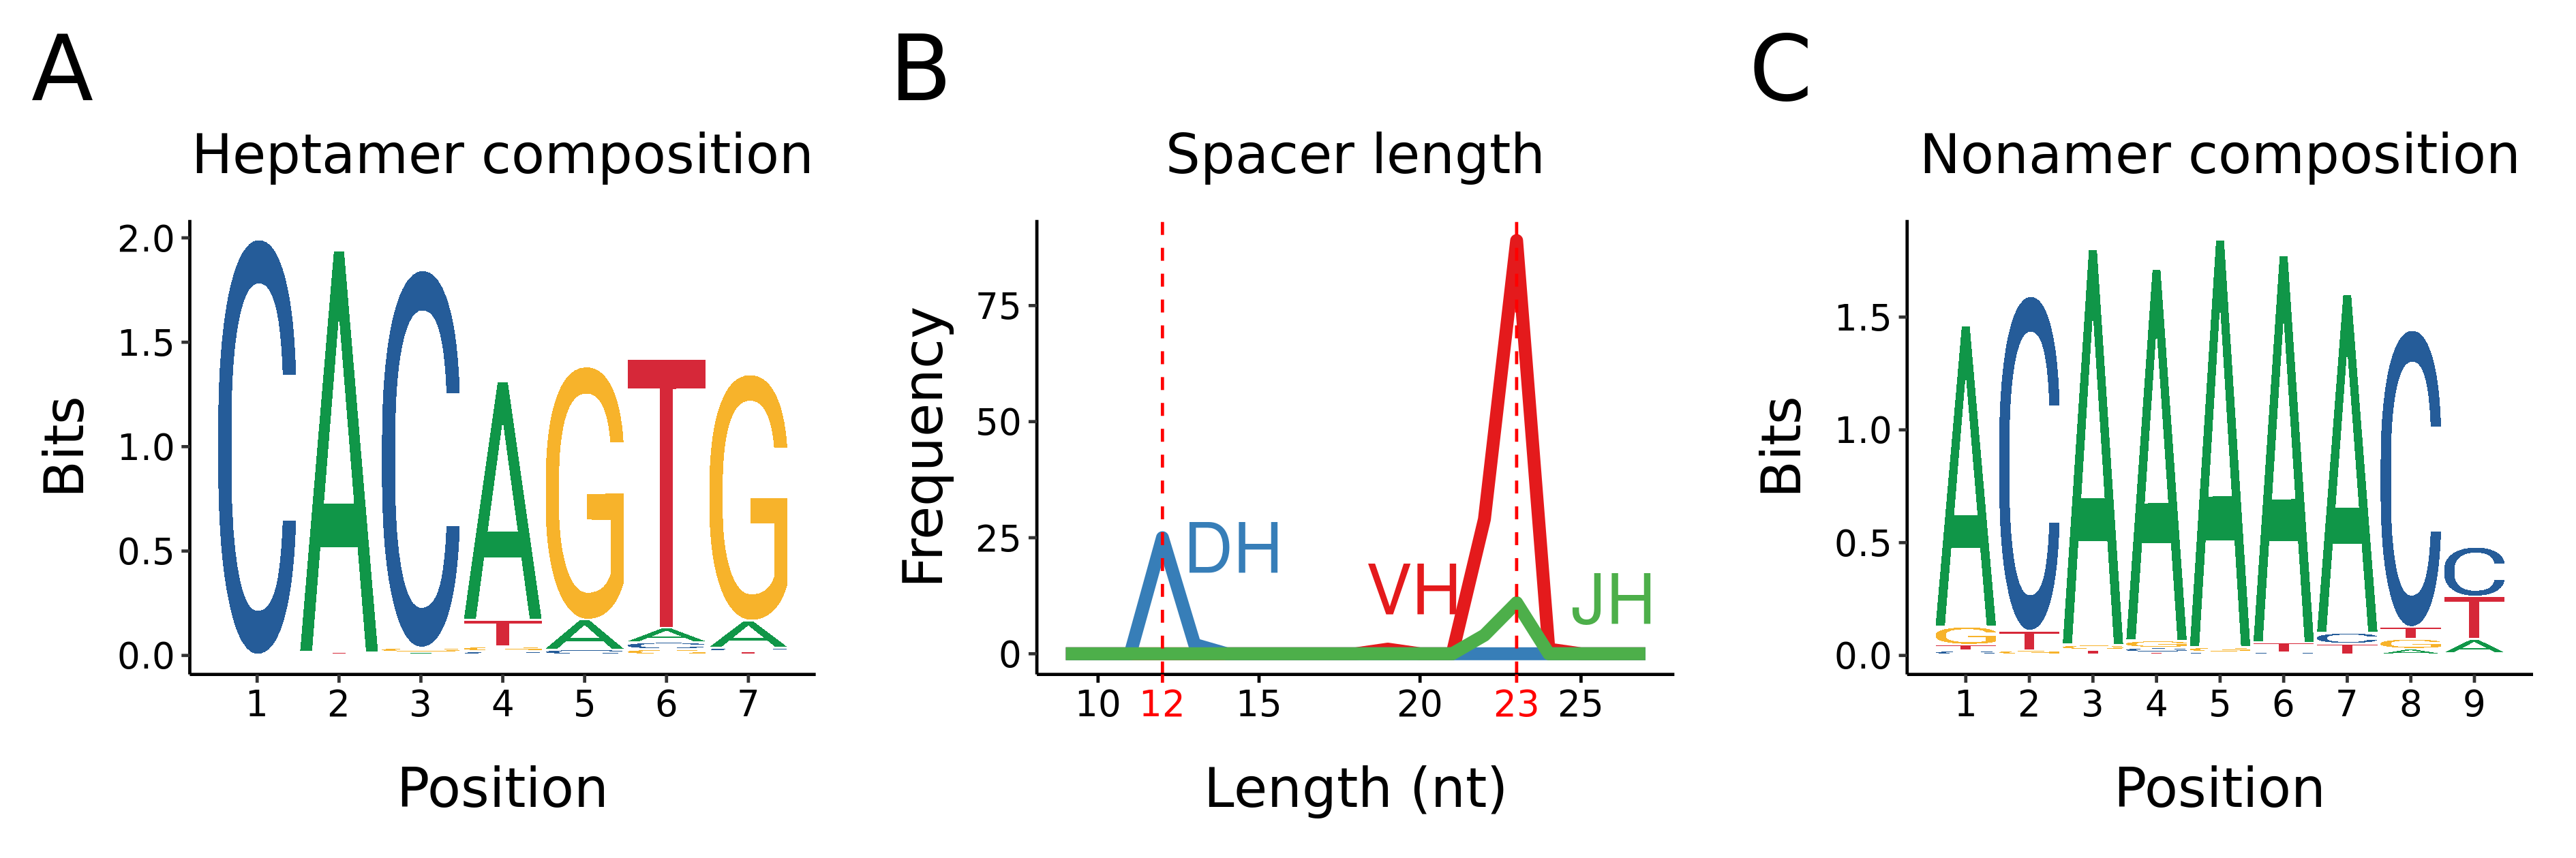
\includegraphics[width=\textwidth]{_Figures/png/xma-new-rss-seqlogo-all}
	\Caption{Recombination signal sequences in the \Xma \igh{} locus}{(A) Sequence composition of conserved heptamer sequences across all \Xma heavy-chain RSSs; (B) length distribution of unconserved spacer sequences in \Xma heavy-chain RSSs; (C) sequence composition of conserved heptamer sequences across all \Xma heavy-chain RSSs.}
	\label{fig:xma-rss-seqlogo-all}
	\vspace{1em}
	\end{figure}
	
	\begin{figure}
	\centering
	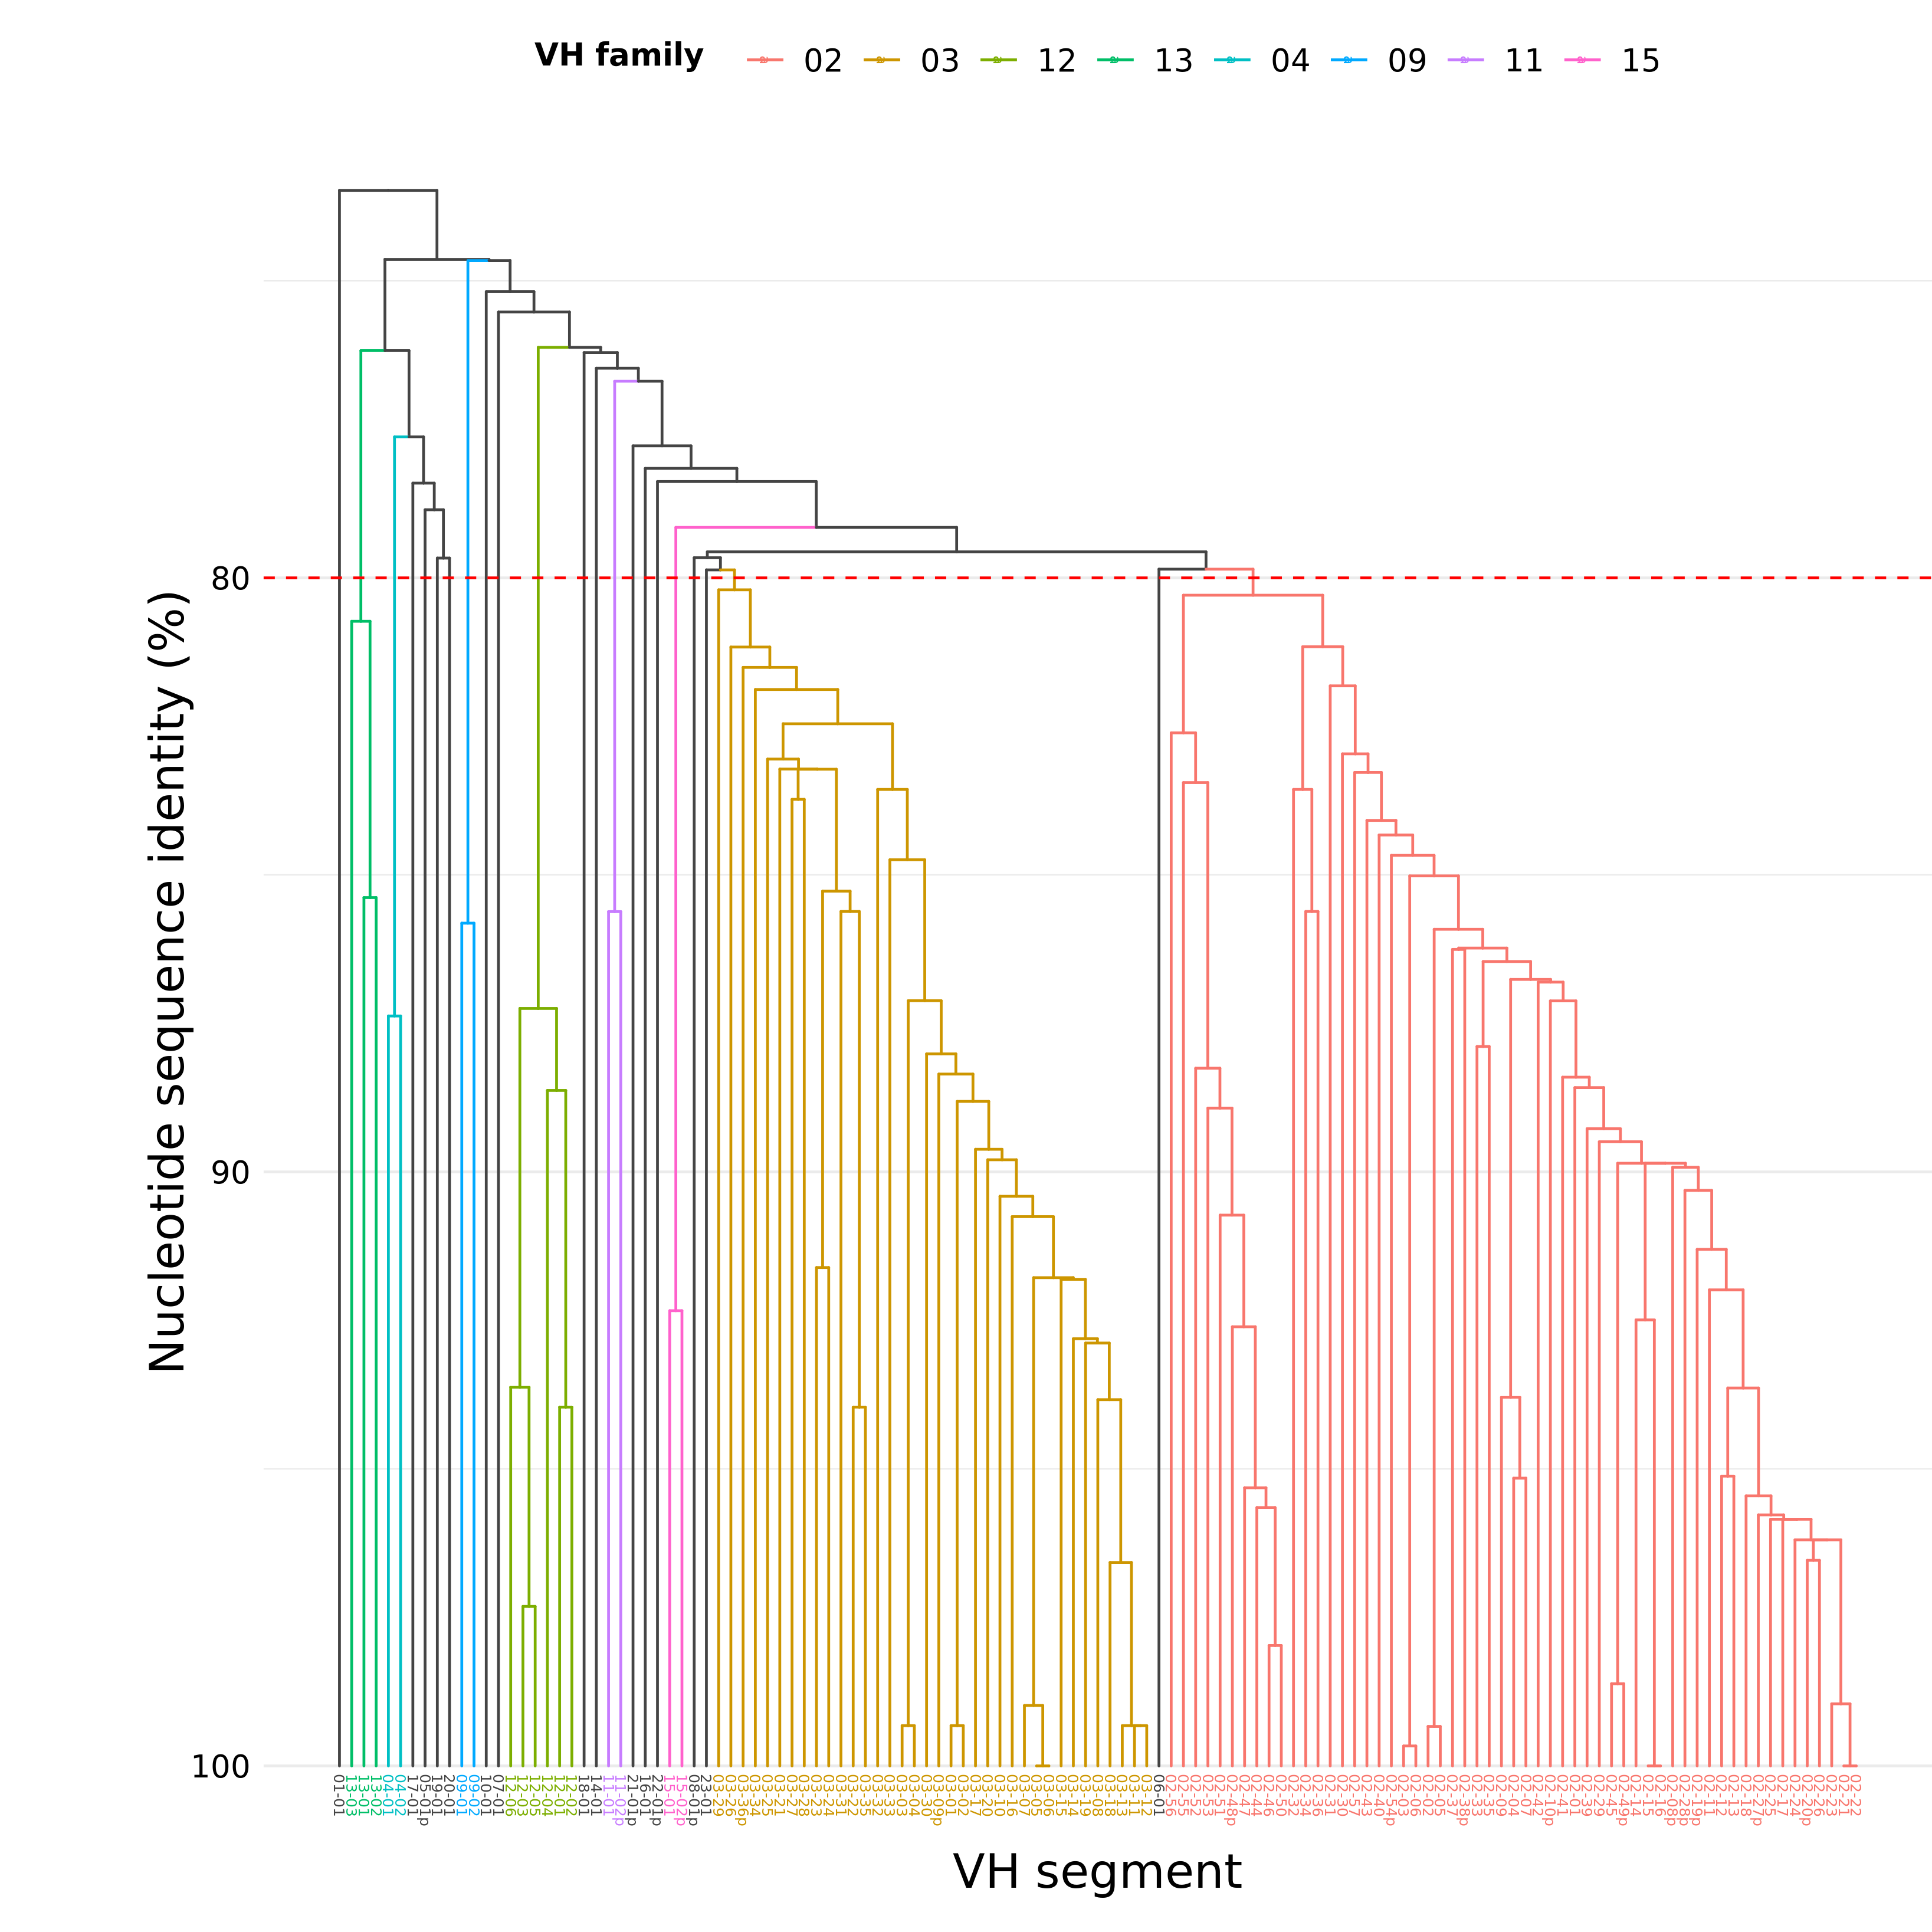
\includegraphics[width=\textwidth]{_Figures/png/xma-vh-families-tree}
	\Caption{Dendrogram of \vh families in the \Xma \igh{} locus}{Dendrogram of sequence similarity of \vh segments in the \Xma locus, arranged by single-linkage clustering on nucleotide sequence identity. The red line indicates the 80\,\% cutoff point for family assignment, while branch colour indicates family membership:  \vh families containing multiple segments are uniquely coloured, while single-segment families are in grey.}
	\label{fig:xma-vh-families-tree}
	\end{figure}
	
	\begin{figure}
	\centering
	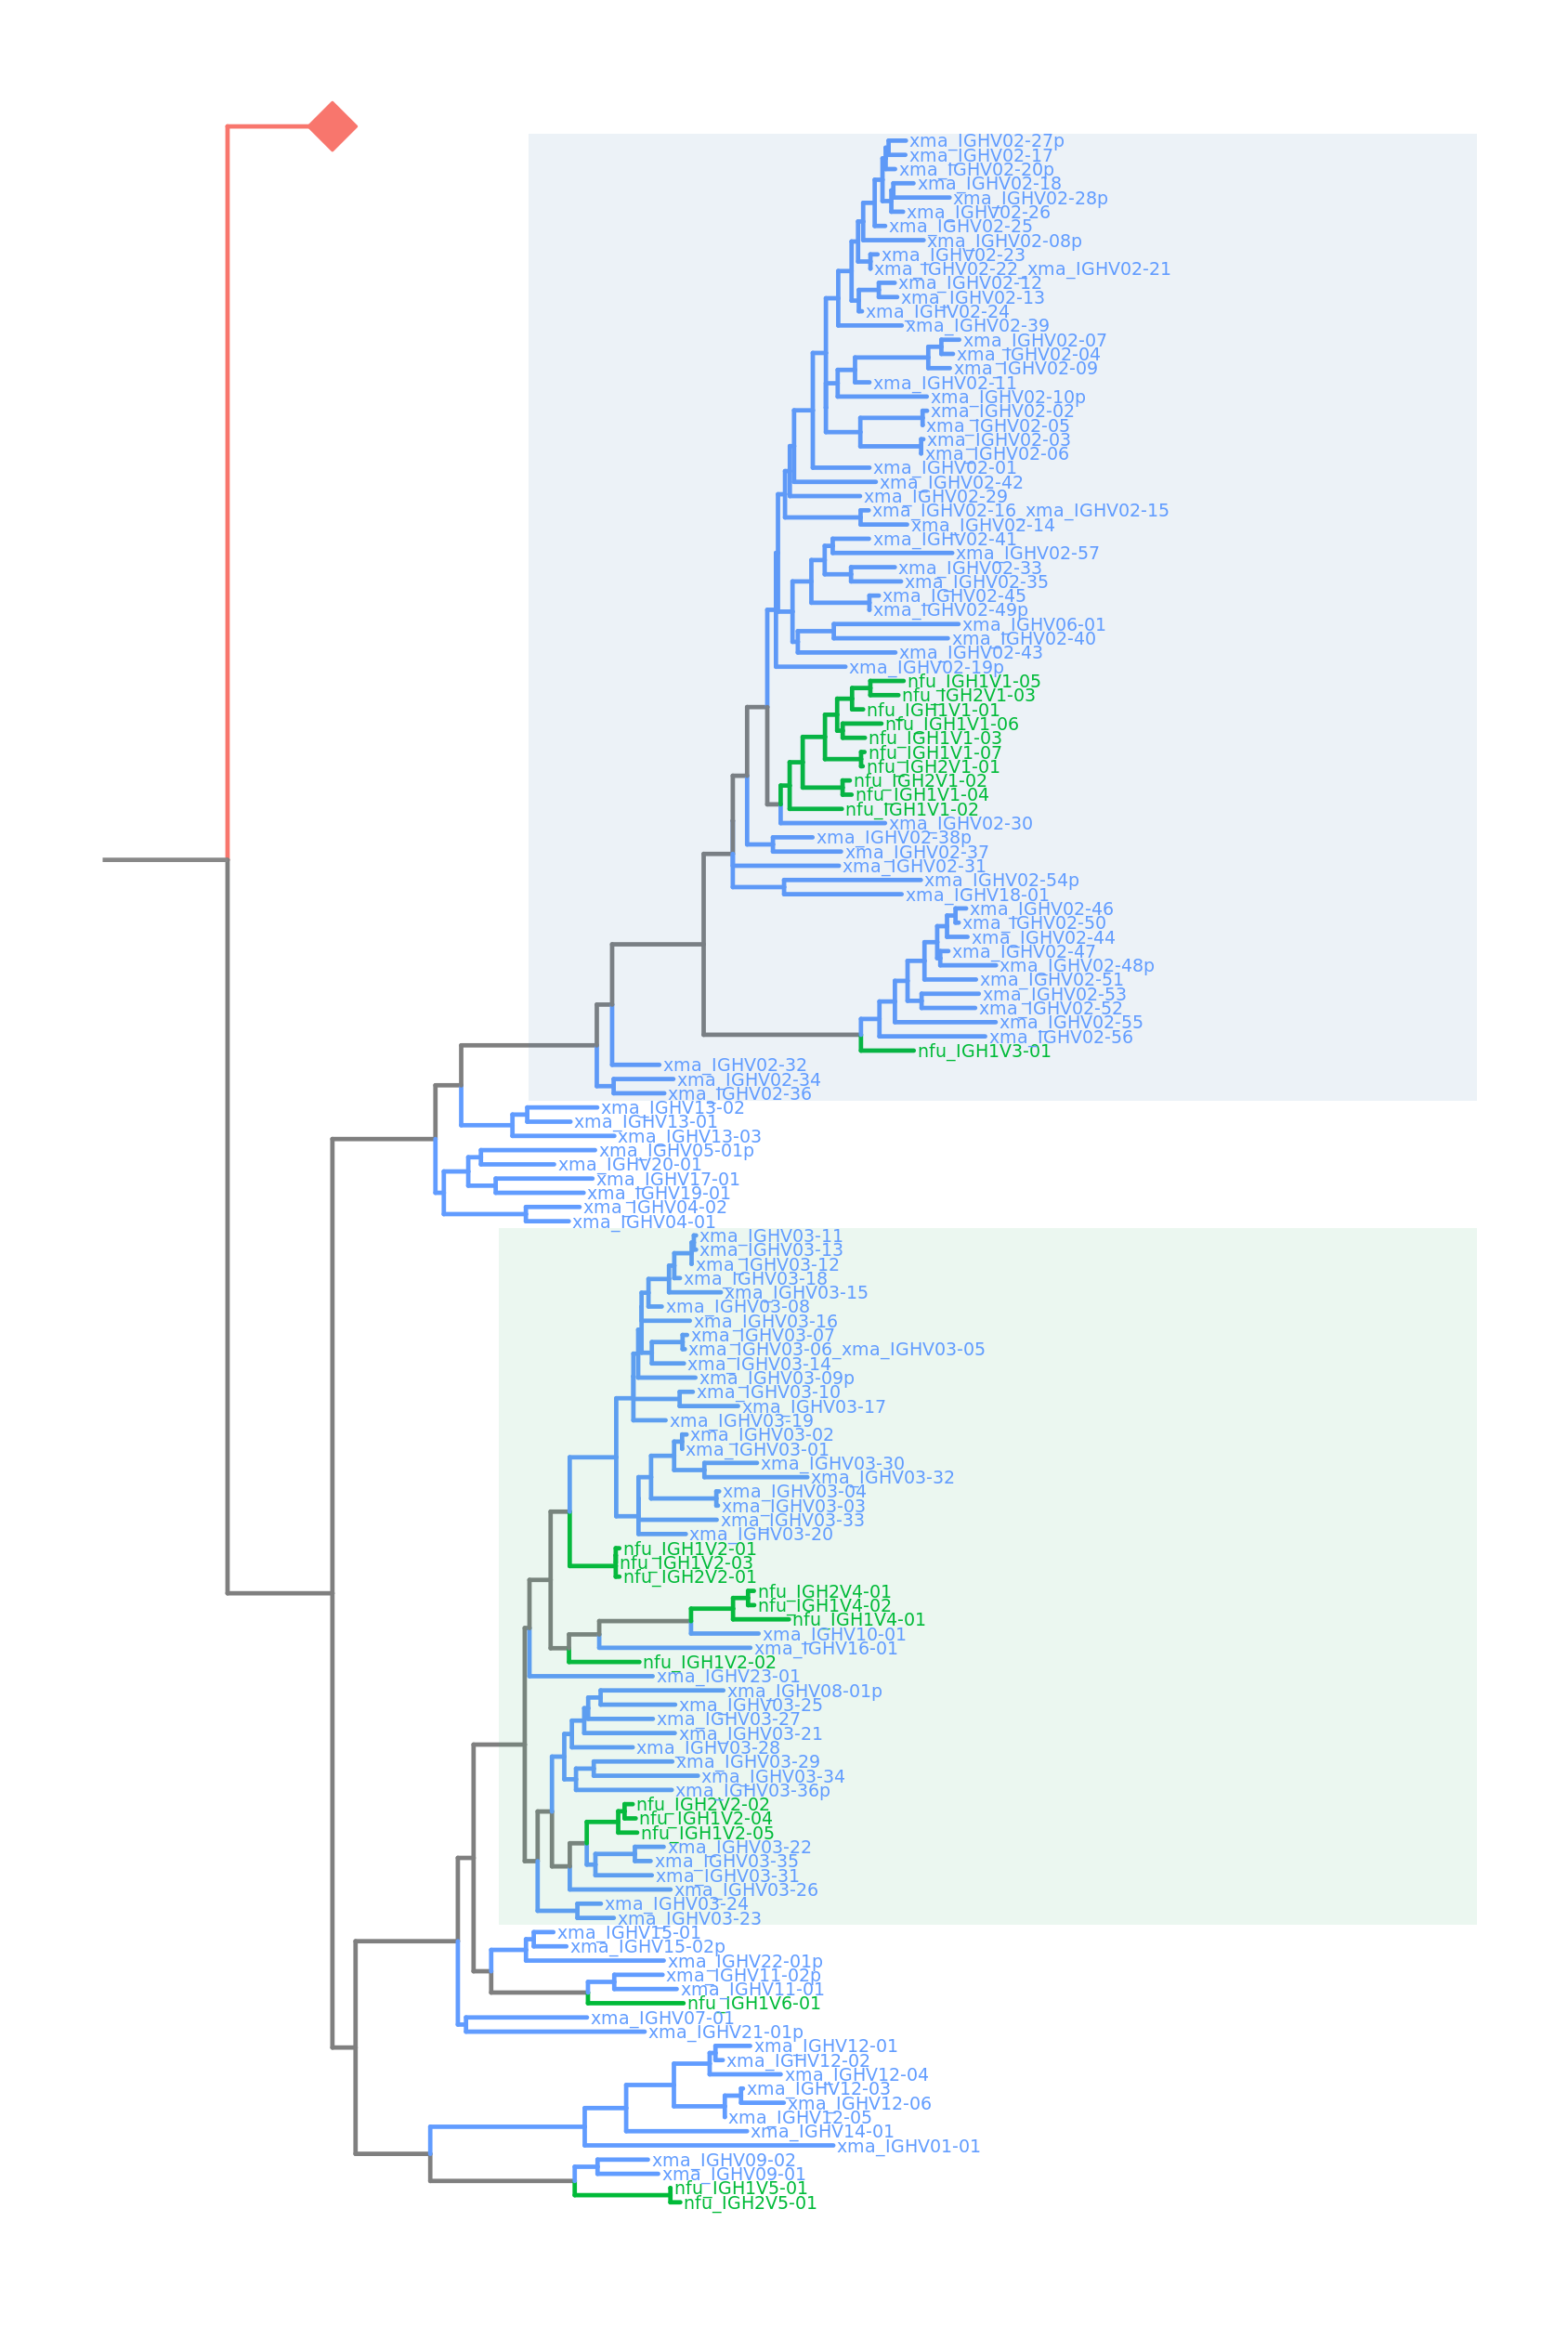
\includegraphics[width=0.8\textwidth]{_Figures/png/nfu-xma-vh-tree-nt.png}
	\Caption{Evolutionary relationships between \vh families in \Xma and \Nfu}{Phylogenetic tree of evolutionary relationships between \igh{} \vh segments in \Nfu and \Xma, as inferred from the nucleotide sequences of \vh segments from both loci. Note the close interrelationship between the largest \vh families in each species (red zone), and similarly between the second-largest families in each species (blue zone). The red diamond indicates the location of the outgroup, which is composed of zebrafish \textit{TRB} V-segments.}
	\label{fig:nfu-xma-vh-tree-nt}
	\end{figure}
		
\FloatBarrier

\clearpage

\section{\igh{} constant-region evolution in the Cyprinodontiformes}
\label{sec:locus_comparative}

The characterised \igh{} loci of \nfu and \xma together reveal a high degree of variability in structure and function across the Atherinomorpha, the parent clade of the Cyprinidontiformes (including \Nfu and \Xma) and medaka (\Cref{fig:species-tree-large-taxa}). Several unusual features (including the loss of \igh{Z}, an inverted sublocus, and an unusual splicing pattern of \igh{M-TM}) are shared between medaka and turquoise killifish, but absent in \Xma (\Cref{fig:species-tree-small}), indicating either an independent origin in the former two species or a reversion to the primitive state in the latter. In addition, the copy number, exon usage and orientation of constant regions of other isotypes differs among the three species, raising the further question of how, when and why these changes occurred. 

In order to investigate a subset of these questions with a greater degree of phylogenetic resolution, I identified and analysed \igh{} constant regions in the genomes of ten additional cyprinodontiform species (\Cref{fig:species-tree-large-taxa}, \Cref{tab:cyprinodontiform-genomes}), as well as in a new and improved genome assembly of medaka (Genbank accession GCA\_002234675.1), using the same methods described for \Nfu and \Xma (\Cref{sec:nfu-locus-constant,sec:nfu-locus-variable}). I then grouped the constant-region exons so identified (\Cref{fig:ch-tree-all}) by order, exon type and spatial proximity to identify contiguous constant-regions, enabling the presence/absence and number of constant regions of each isotype to be estimated for each species. The results of this analysis (\Cref{fig:multispecies-ch-regions}, \Cref{tab:multispecies-ch-regions-1,tab:multispecies-ch-regions-2,tab:multispecies-ch-regions-3}) demonstrate that every species investigated possesses at least one complete \igh{M} and \igh{D} constant region in tandem, with several species exhibiting multiple such regions. Apart from \Nfu and medaka, only \textit{Nothobranchius orthonotus} was identified as clearly possessing adjacent constant regions in opposite orientation, indicating the presence of at least one sublocus in antisense; however, the fragmented nature of the \igh{} locus assembly in many analysed species prevented a confident exclusion of such configurations in other cases.

\begin{table}[bh!]
\centering
\begin{threeparttable}
\begin{tabular}{>{\itshape}l>{\itshape}llc}\toprule
\textnormal{\textbf{Genus}} & \textnormal{\textbf{Species}} & \textbf{Common Name} & \textbf{GenBank Assembly Accession}\\\midrule
Nothobranchius & furzeri & Turquoise killifish & NA\tnote{1}\\\midrule
Xiphophorus & maculatus & Southern platyfish & GCA\_002775205.2\\
Austrofundulus & limnaeus & -- & GCA\_001266775.1\\
Fundulus & heteroclitus & Mummichog & GCA\_000826765.1\\
Poecilia & formosa & Amazon molly & GCA\_000485575.1\\
Poecilia & reticulata & Guppy & GCA\_000633615.1\\
Cyprinodon & variegatus & Sheepshead minnow & GCA\_000732505.1\\
Kryptolebias & marmoratus & Mangrove rivulus & GCA\_001649575.1\\\midrule
Aphyosemion & australe & Lyretail panchax & NA\tnote{2}\\
Callopanchax & toddi & -- & NA\tnote{2}\\
Pachypanchax & playfairii & Golden panchax & NA\tnote{2}\\
Nothobranchius & orthonotus & Spotted killifish & NA\tnote{2}\\\midrule
Oryzias & latipes & Medaka & GCA\_002234675.1\\
\bottomrule\end{tabular}
\begin{tablenotes}
\item[1] Willemsen \textit{et al.} \parencite{willemsen2019popgen}
\item[2] Cui \textit{et al.} \parencite{cui2019annual}
\end{tablenotes}
\end{threeparttable}
\vspace{0.5em}
\caption{Genome assemblies used to identify \igh{} locus sequences in cyprinodontiform fishes}
\label{tab:cyprinodontiform-genomes}
\end{table}

\begin{figure}
\centering
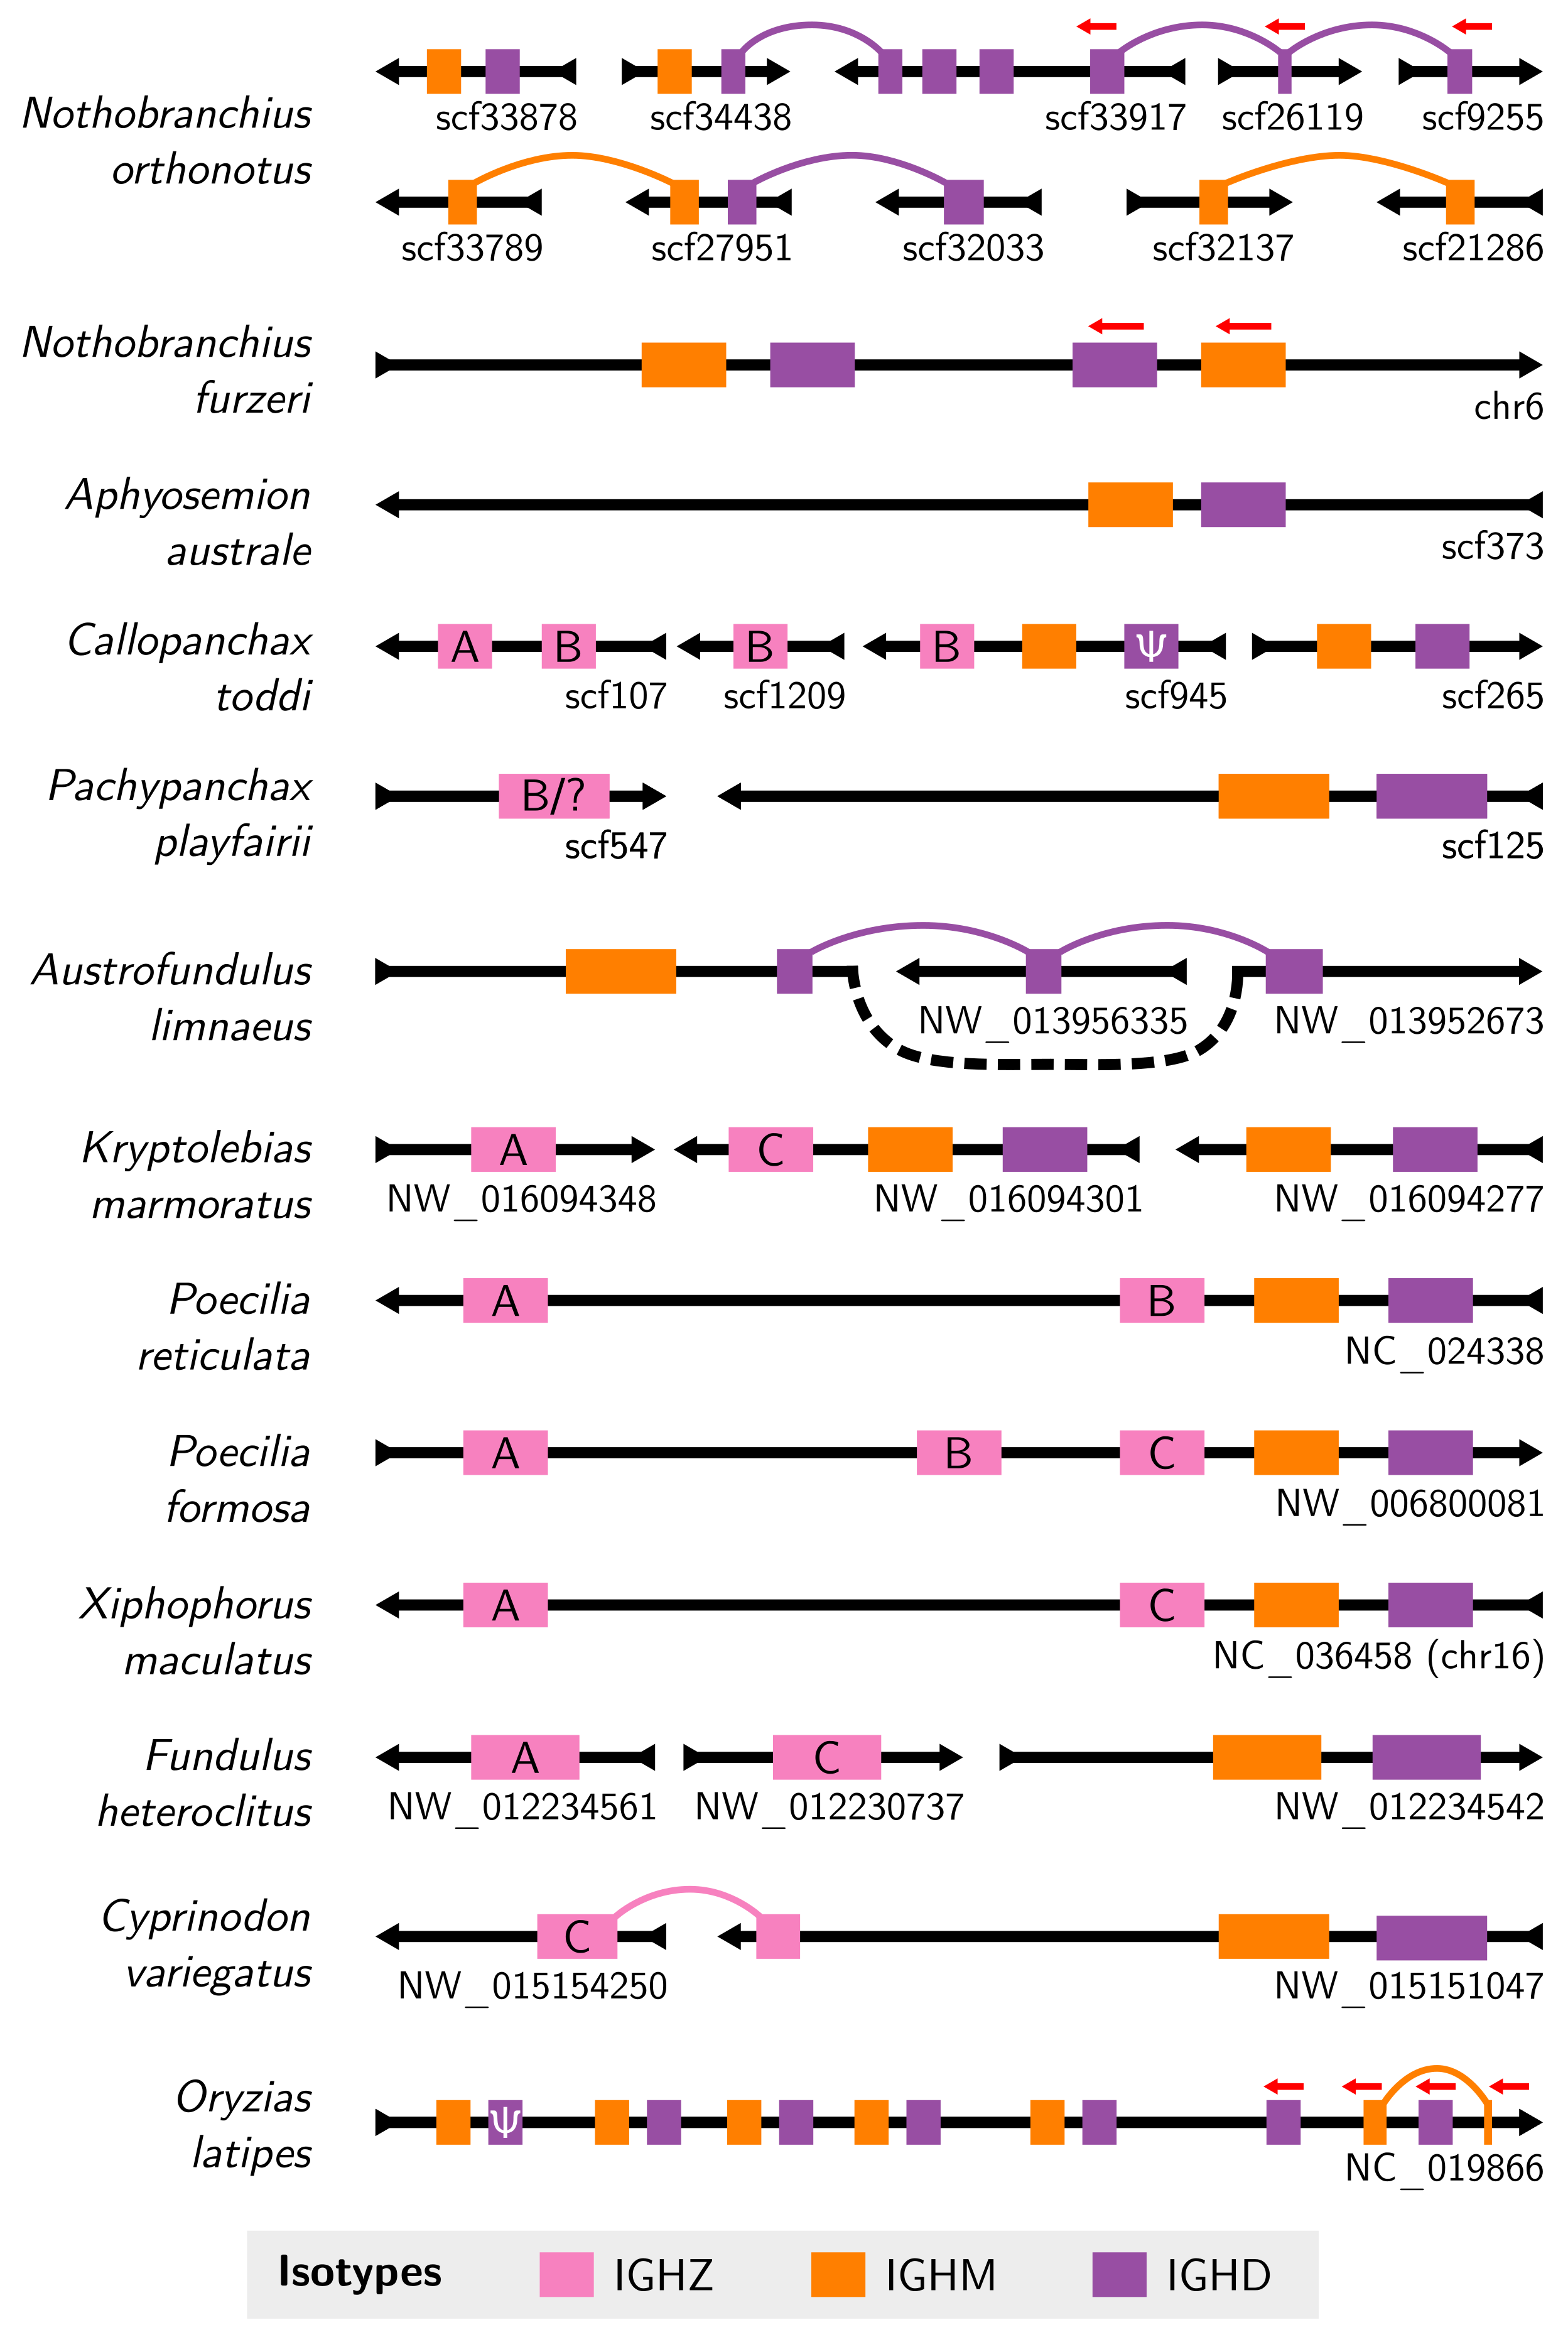
\includegraphics[width=0.9\textwidth]{_Figures/png_edited/multispecies-ch-regions}
\Caption{Constant-region organisation in the Atherinomorpha}{Schematic of \igh{} constant regions in the genomes of thirteen species from the Atherinomorpha. Scaffold orientation is given by the black arrows; constant regions are oriented left-to-right unless otherwise specified (red arrows). Links between regions on different scaffolds indicate that exons from what appears to be the same constant region are distributed across multiple scaffolds in the order indicated; the order of unlinked scaffolds is arbitrary. The isotype of each region is given by its colour; \igh{Z} regions are further annotated with their subclass (\Cref{fig:species-tree-large-ighz}). Clearly pseudogenised constant regions are indicated by $\Psi$. Isotype length, scaffold length, and scaffold position are not to scale. Variable regions and lone, isolated constant-region exons are not shown.}
\label{fig:multispecies-ch-regions}
\end{figure}

In addition to at least one \igh{M} and \igh{D} constant region, the majority of species analysed (8 out of 13) were also found to possess at least one complete \igh{Z} constant region; of the exceptions, \species{A.}{limnaeus} exhibits an orphaned, pseudogenised \igh{Z-TM1} exon but no \cz{} exons in the current genome assembly (\Cref{fig:multispecies-ch-regions}, \Cref{tab:multispecies-ch-regions-2}), while \species{O.}{latipes}, \species{A.}{australe}, \Nfu and \species{N.}{orthonotus} possess no \igh{Z} exons at all. Annotating the tree from \Cref{fig:species-tree-large-taxa} with the \igh{Z} status of each species (\Cref{fig:species-tree-large-ighz}) confirms that the loss of \igh{Z} in turquoise killifish (and related species) and medaka represent two distinct deletion events, with \textit{Austrofundulus limnaeus} potentially representing a second independent loss of \igh{Z} within the Cyprinodontiformes and a third within the Atherinomorpha.

\begin{figure}
\centering
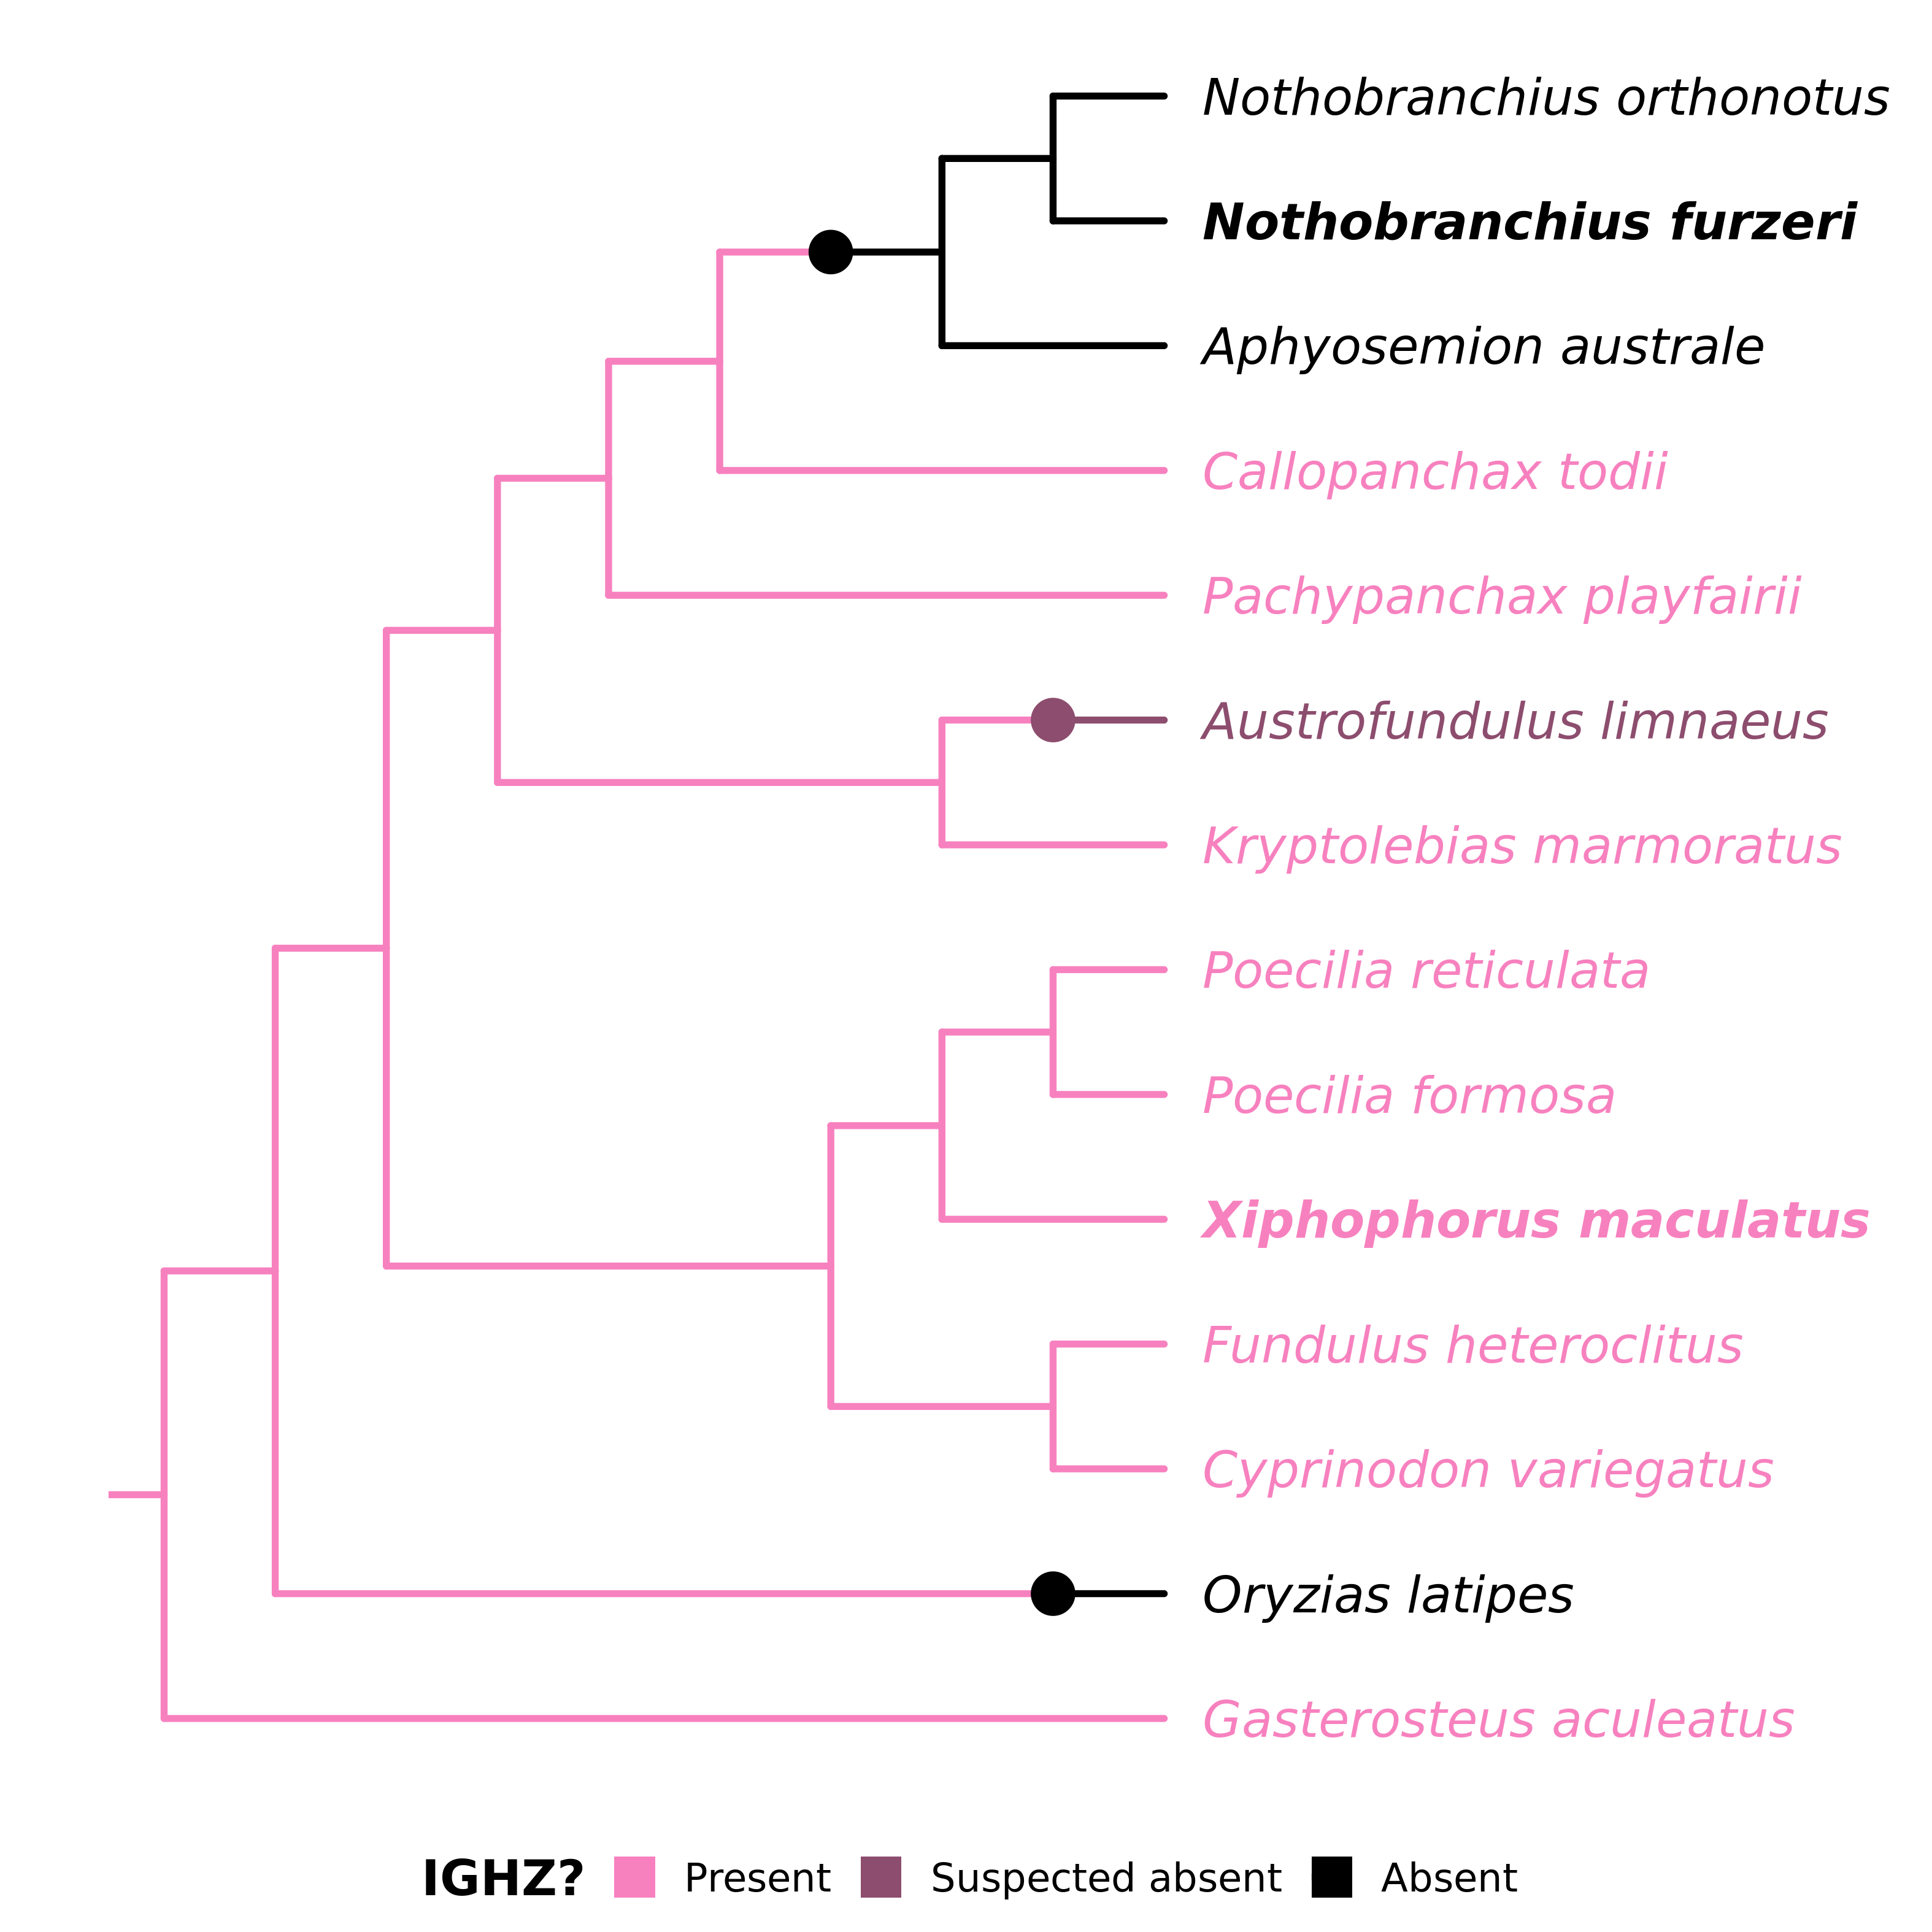
\includegraphics[width=0.9\textwidth]{_Figures/png/species-tree-large-ighz}
\Caption{\igh{Z} has been lost multiple times independently in the Atherinomorpha}{Cladogram of species reproduced from \Cref{fig:species-tree-large-taxa}, annotated according to the known (tip nodes) or inferred (internal nodes) presence or absence of intact \igh{Z} constant regions in each species. Large coloured points on the cladogram denote sites of hypothesised state changes; \igh{Z} is assumed to be primitively present in the clade and losses to be irreversible. The currently-available genome assembly of \textit{A. limnaeus} (dark pink) contains one pseudogenised \igh{Z-TM1} exon and no \cz{} exons.}
\label{fig:species-tree-large-ighz}
\end{figure}

Apart from its repeated loss within the lineage, a second striking feature of \igh{Z} within the Cyprinodontiformes is its frequent presence in multiple copies per \igh{} locus, with a geometric mean of 1.929 regions per \igh{Z}-bearing locus. On average (geometric mean), the species analysed have approximately 1.62 \igh{Z} constant regions per \igh{M} constant region, and the same ratio vs \igh{D}, suggesting a more complex evolutionary history than can be captured by a simple presence/absence metric. Concordantly, phylogenetic analysis (\Cref{fig:multispecies-cz-tree}, tree built using \program{PRANK} and \program{RAxML} on concatenated \cz{1}--\cz{4} exon sequences) reveals three distinct lineages (or subclasses) of \igh{Z} constant regions in the Cyprinidontiformes, \igh{ZA} to \textit{C}, each of which is present in multiple different species and appears to have been present in the common ancestor of the eight \igh{Z}-bearing species analysed (\Cref{fig:multispecies-cz-subclasses}).

\begin{figure}
	\centering
	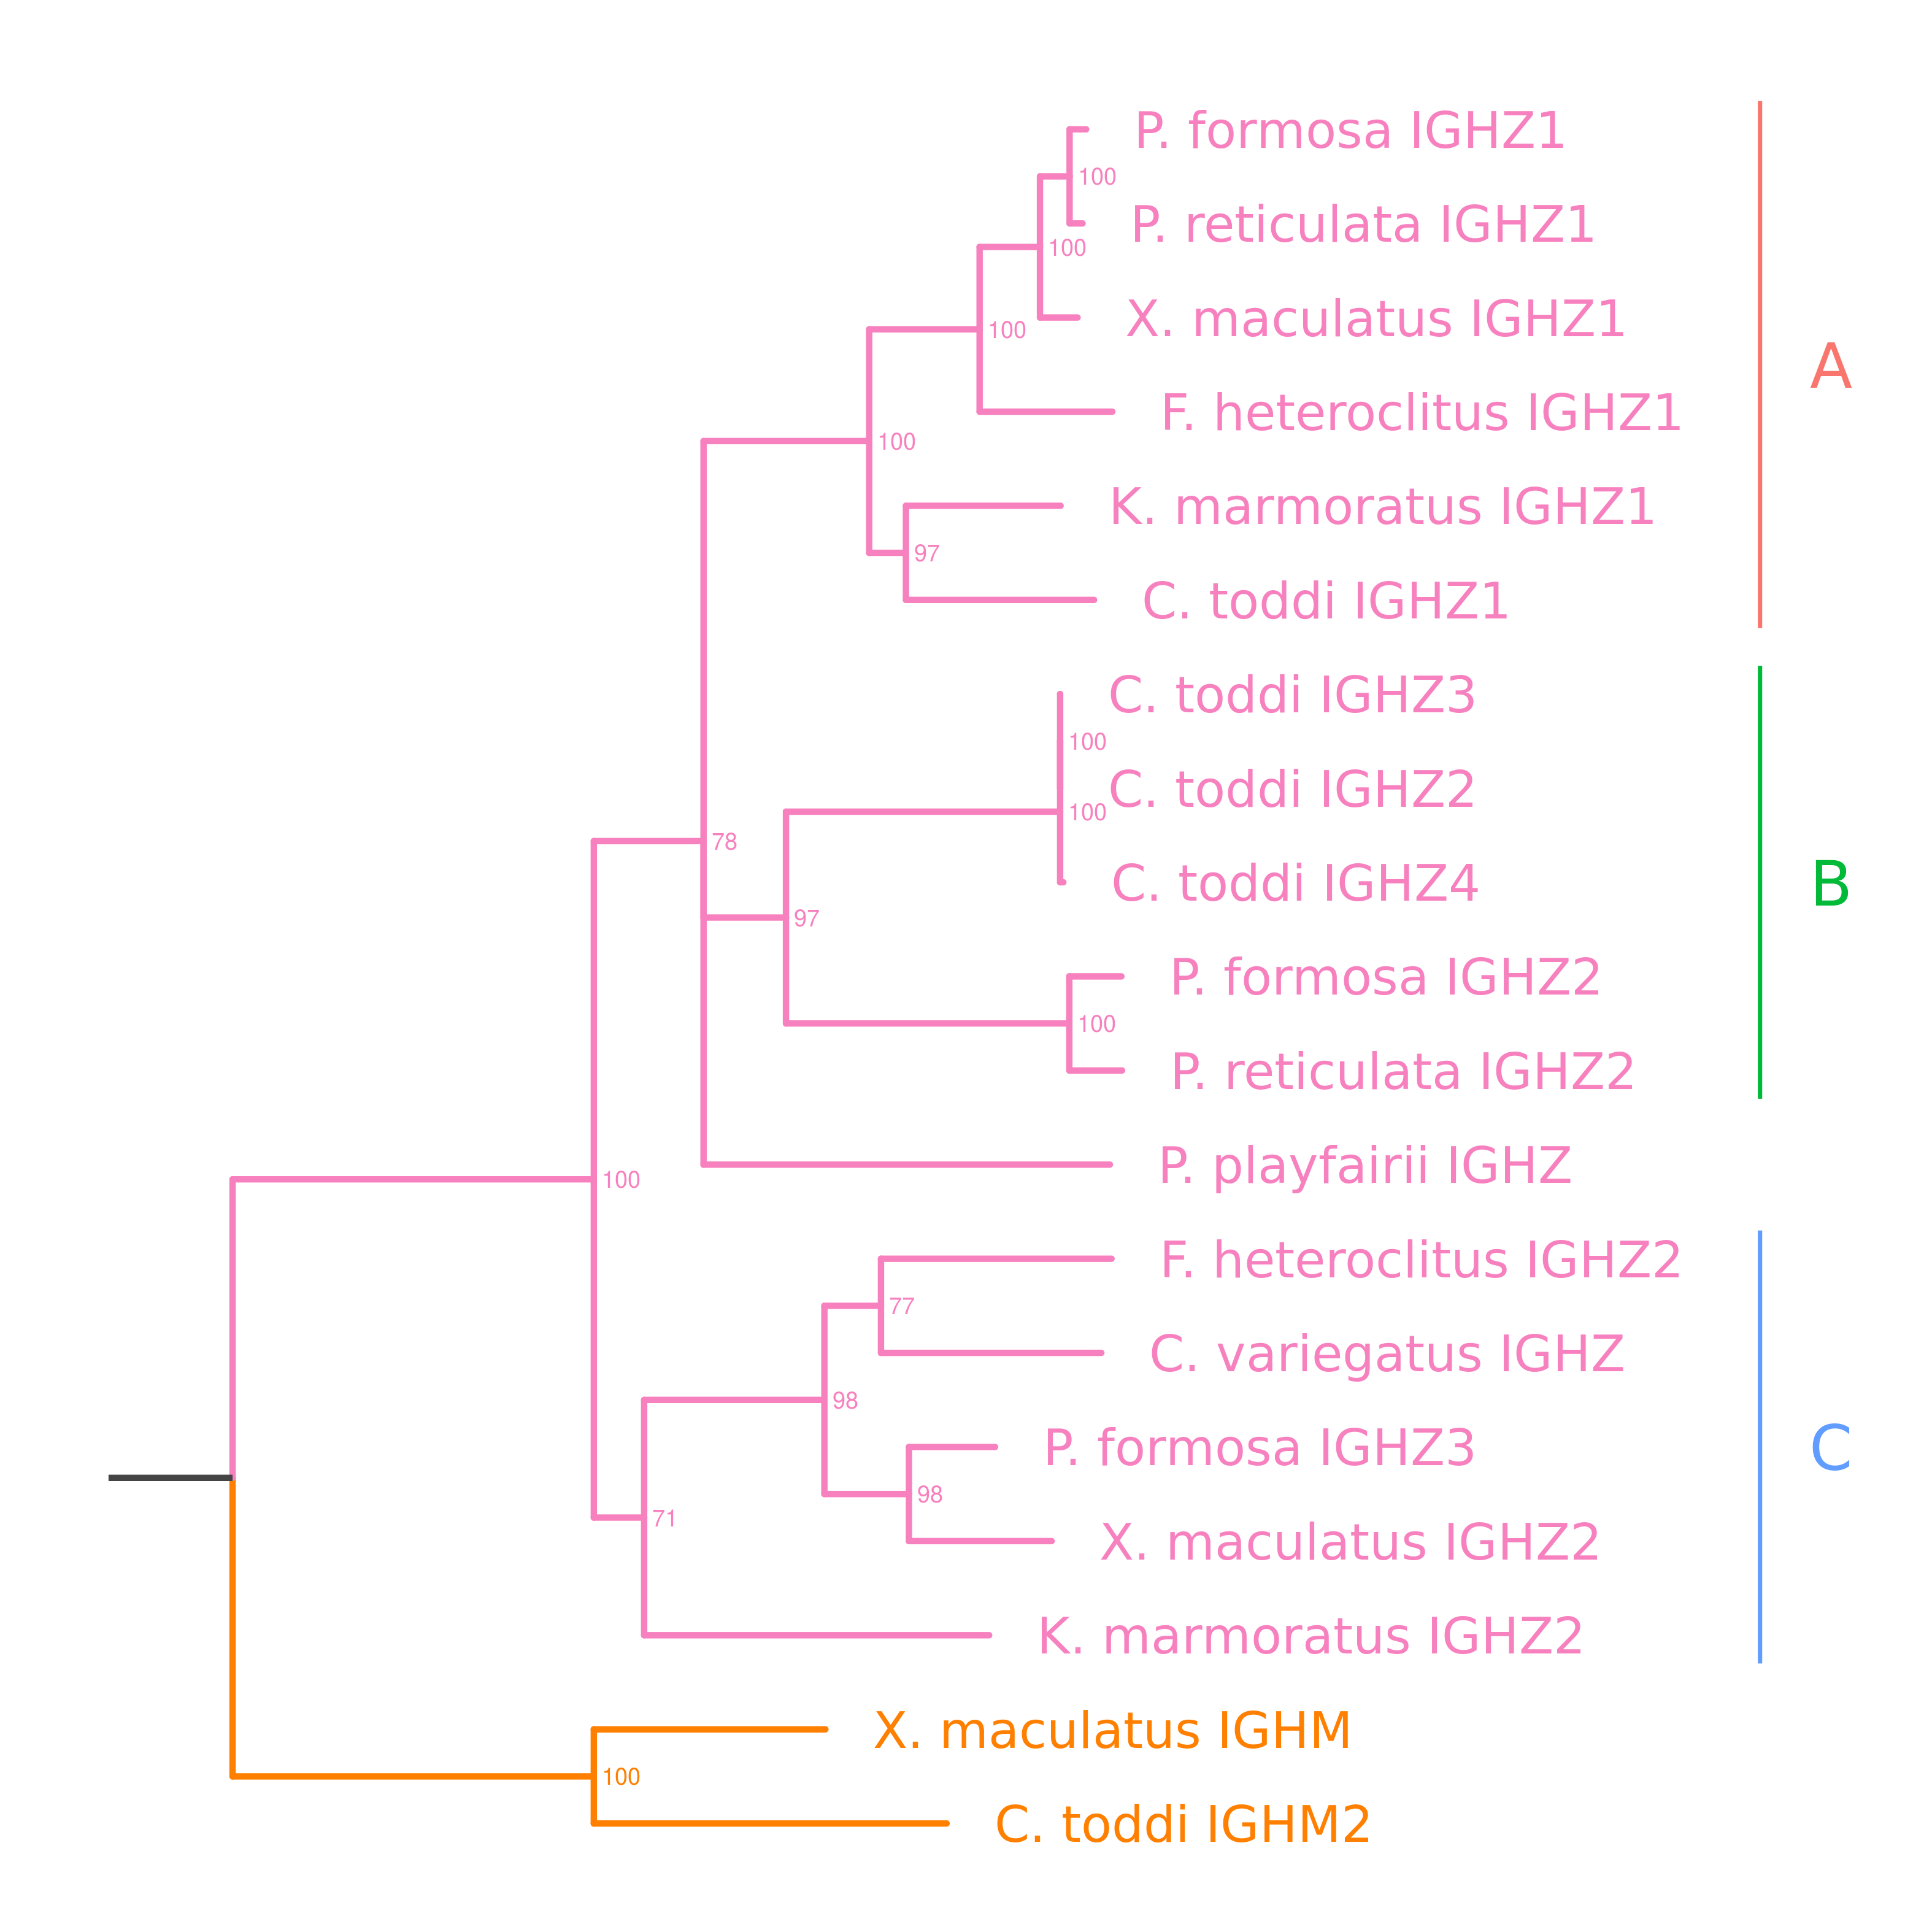
\includegraphics[width=0.9\textwidth]{_Figures/png/multispecies-cz-tree}
	\Caption{\igh{Z} constant regions in the Cyprinodontiformes constitute three distinct subclasses}{Phylogram of concatenated \cz{1}--\cz{4} nucleotide sequences from \igh{Z}-bearing species in \Cref{tab:cyprinodontiform-genomes}, with \cm{1}--\cm{4} sequences from two species as an outgroup (in orange). Nodes with bootstrap support of less than 65\,\% are collapsed into polytomies. Major clades (A--C) are annotated on the right. Support values indicate the result of rapid bootstrapping by \program{RAxML} across 1000 replicates.}
	\label{fig:multispecies-cz-tree}
\end{figure}

\begin{figure}
\centering
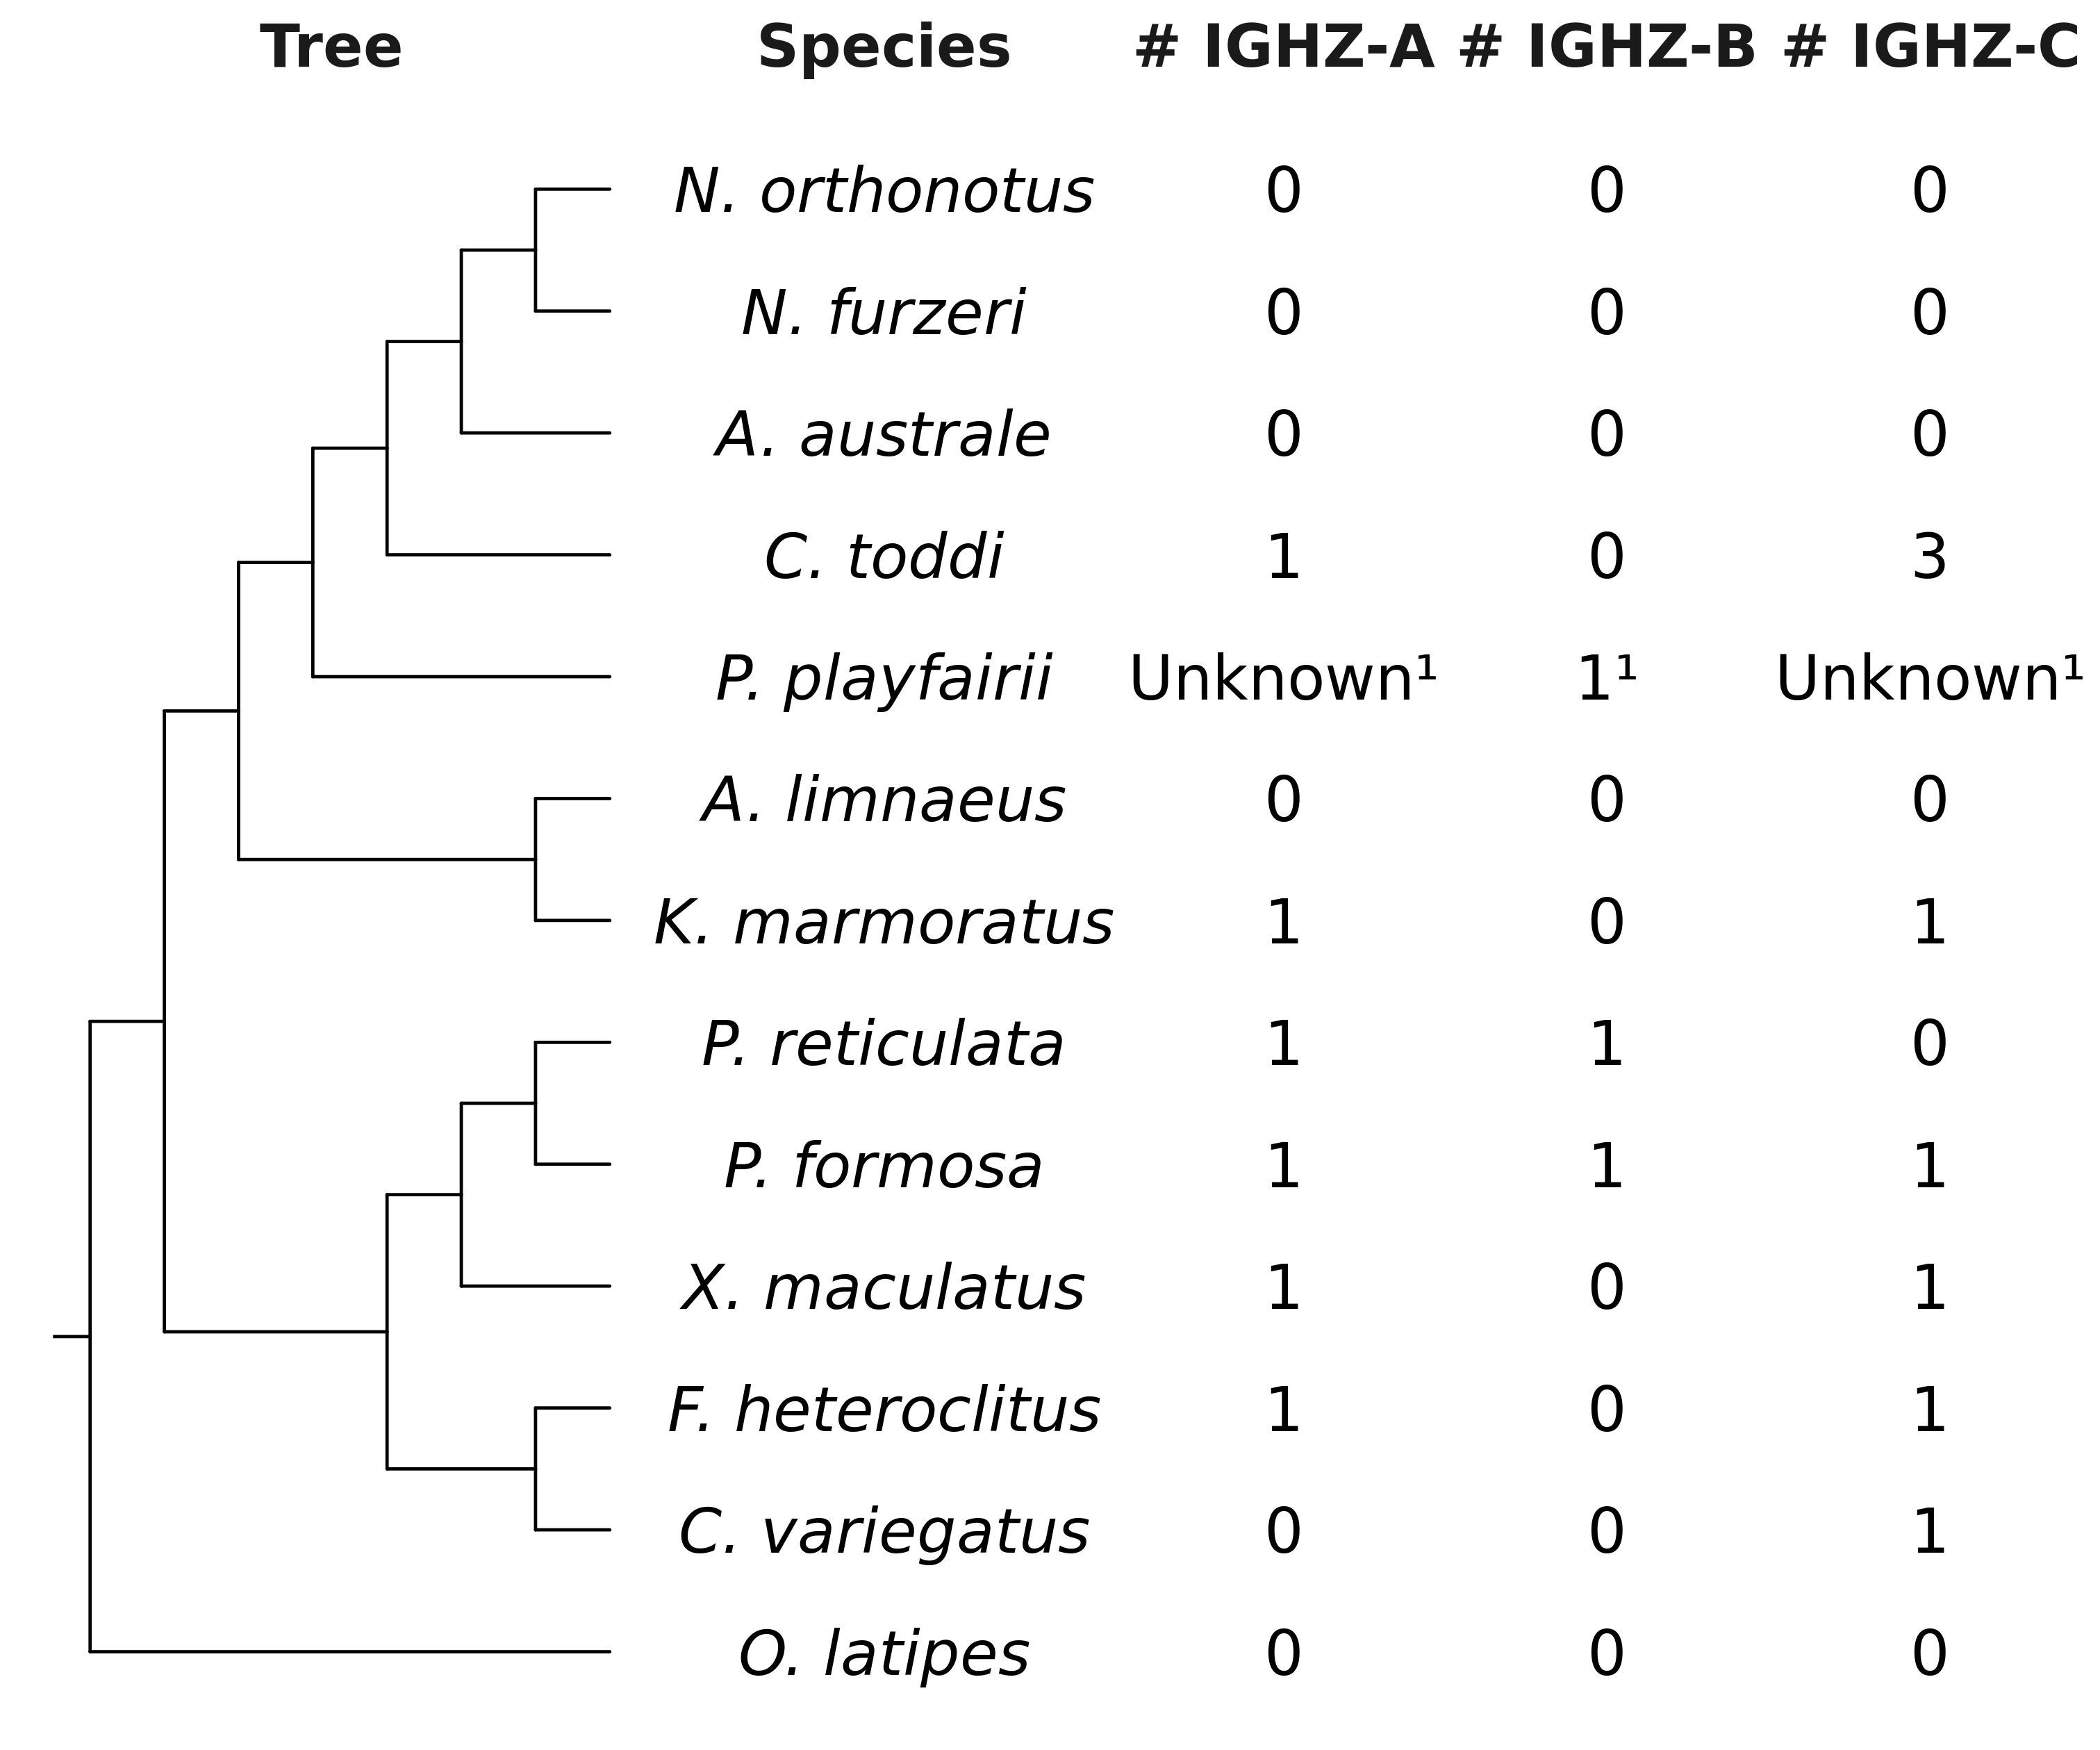
\includegraphics[width=0.8\textwidth]{_Figures/png/multispecies-cz-subclasses}
\begin{minipage}{0.7\textwidth}
\footnotesize
\begin{threeparttable}
\begin{tablenotes}
\item[1] \textit{P. playfairii} \igh{Z} \cz{1}--\cz{2} appear to be derived from \igh{Z-B}, while the other exons are of uncertain subclass origin (\Cref{fig:ppl-cz-aln}).
\end{tablenotes}
\end{threeparttable}
\end{minipage}
\Caption{Distribution of \igh{Z} subclasses in the Atherinomorpha}{Cladogram of atherinomorph species with characterised \igh{} constant regions, annotated with the number of regions belonging to each \igh{Z} isotype in each species. All three subclasses are present in at least one species in both major branches of the cyprinodontiform clade, suggesting that they were all present in the common ancestor of this grouping.}
\label{fig:multispecies-cz-subclasses}
\end{figure}


Only one \igh{Z} constant region from the analysed species could not be confidently assigned to one of these three subclasses, namely the single \igh{Z} of \species{Pachypanchax}{playfairii} (\Cref{fig:multispecies-cz-tree}). In order to more closely investigate the relationships of \igh{Z} in this species, I aligned the exon sequences of \species{P.}{playfairii} \cz{1}--\cz{4} separately to the \cz{} exons of all other \igh{Z}-bearing species and plotted the distribution of alignment scores in each case (\Cref{fig:ppl-cz-aln}). The results show a striking difference in alignment behaviour between the exons, with \cz{1} and \cz{2} aligning significantly more strongly to exons from the B subclass and \cz{3} and \cz{4} showing more ambiguous affinity for either A- or C-subclass sequences. This unexpected behaviour indicates that the \species{P.}{playfairii} \igh{Z} sequence is the result of a deletion or fusion event combining the first two exons of a B-subclass \igh{Z} constant region with the latter exons of a constant region from another subclass, resulting in a chimeric gene with ambiguous ancestry.

\begin{figure}
	\centering
	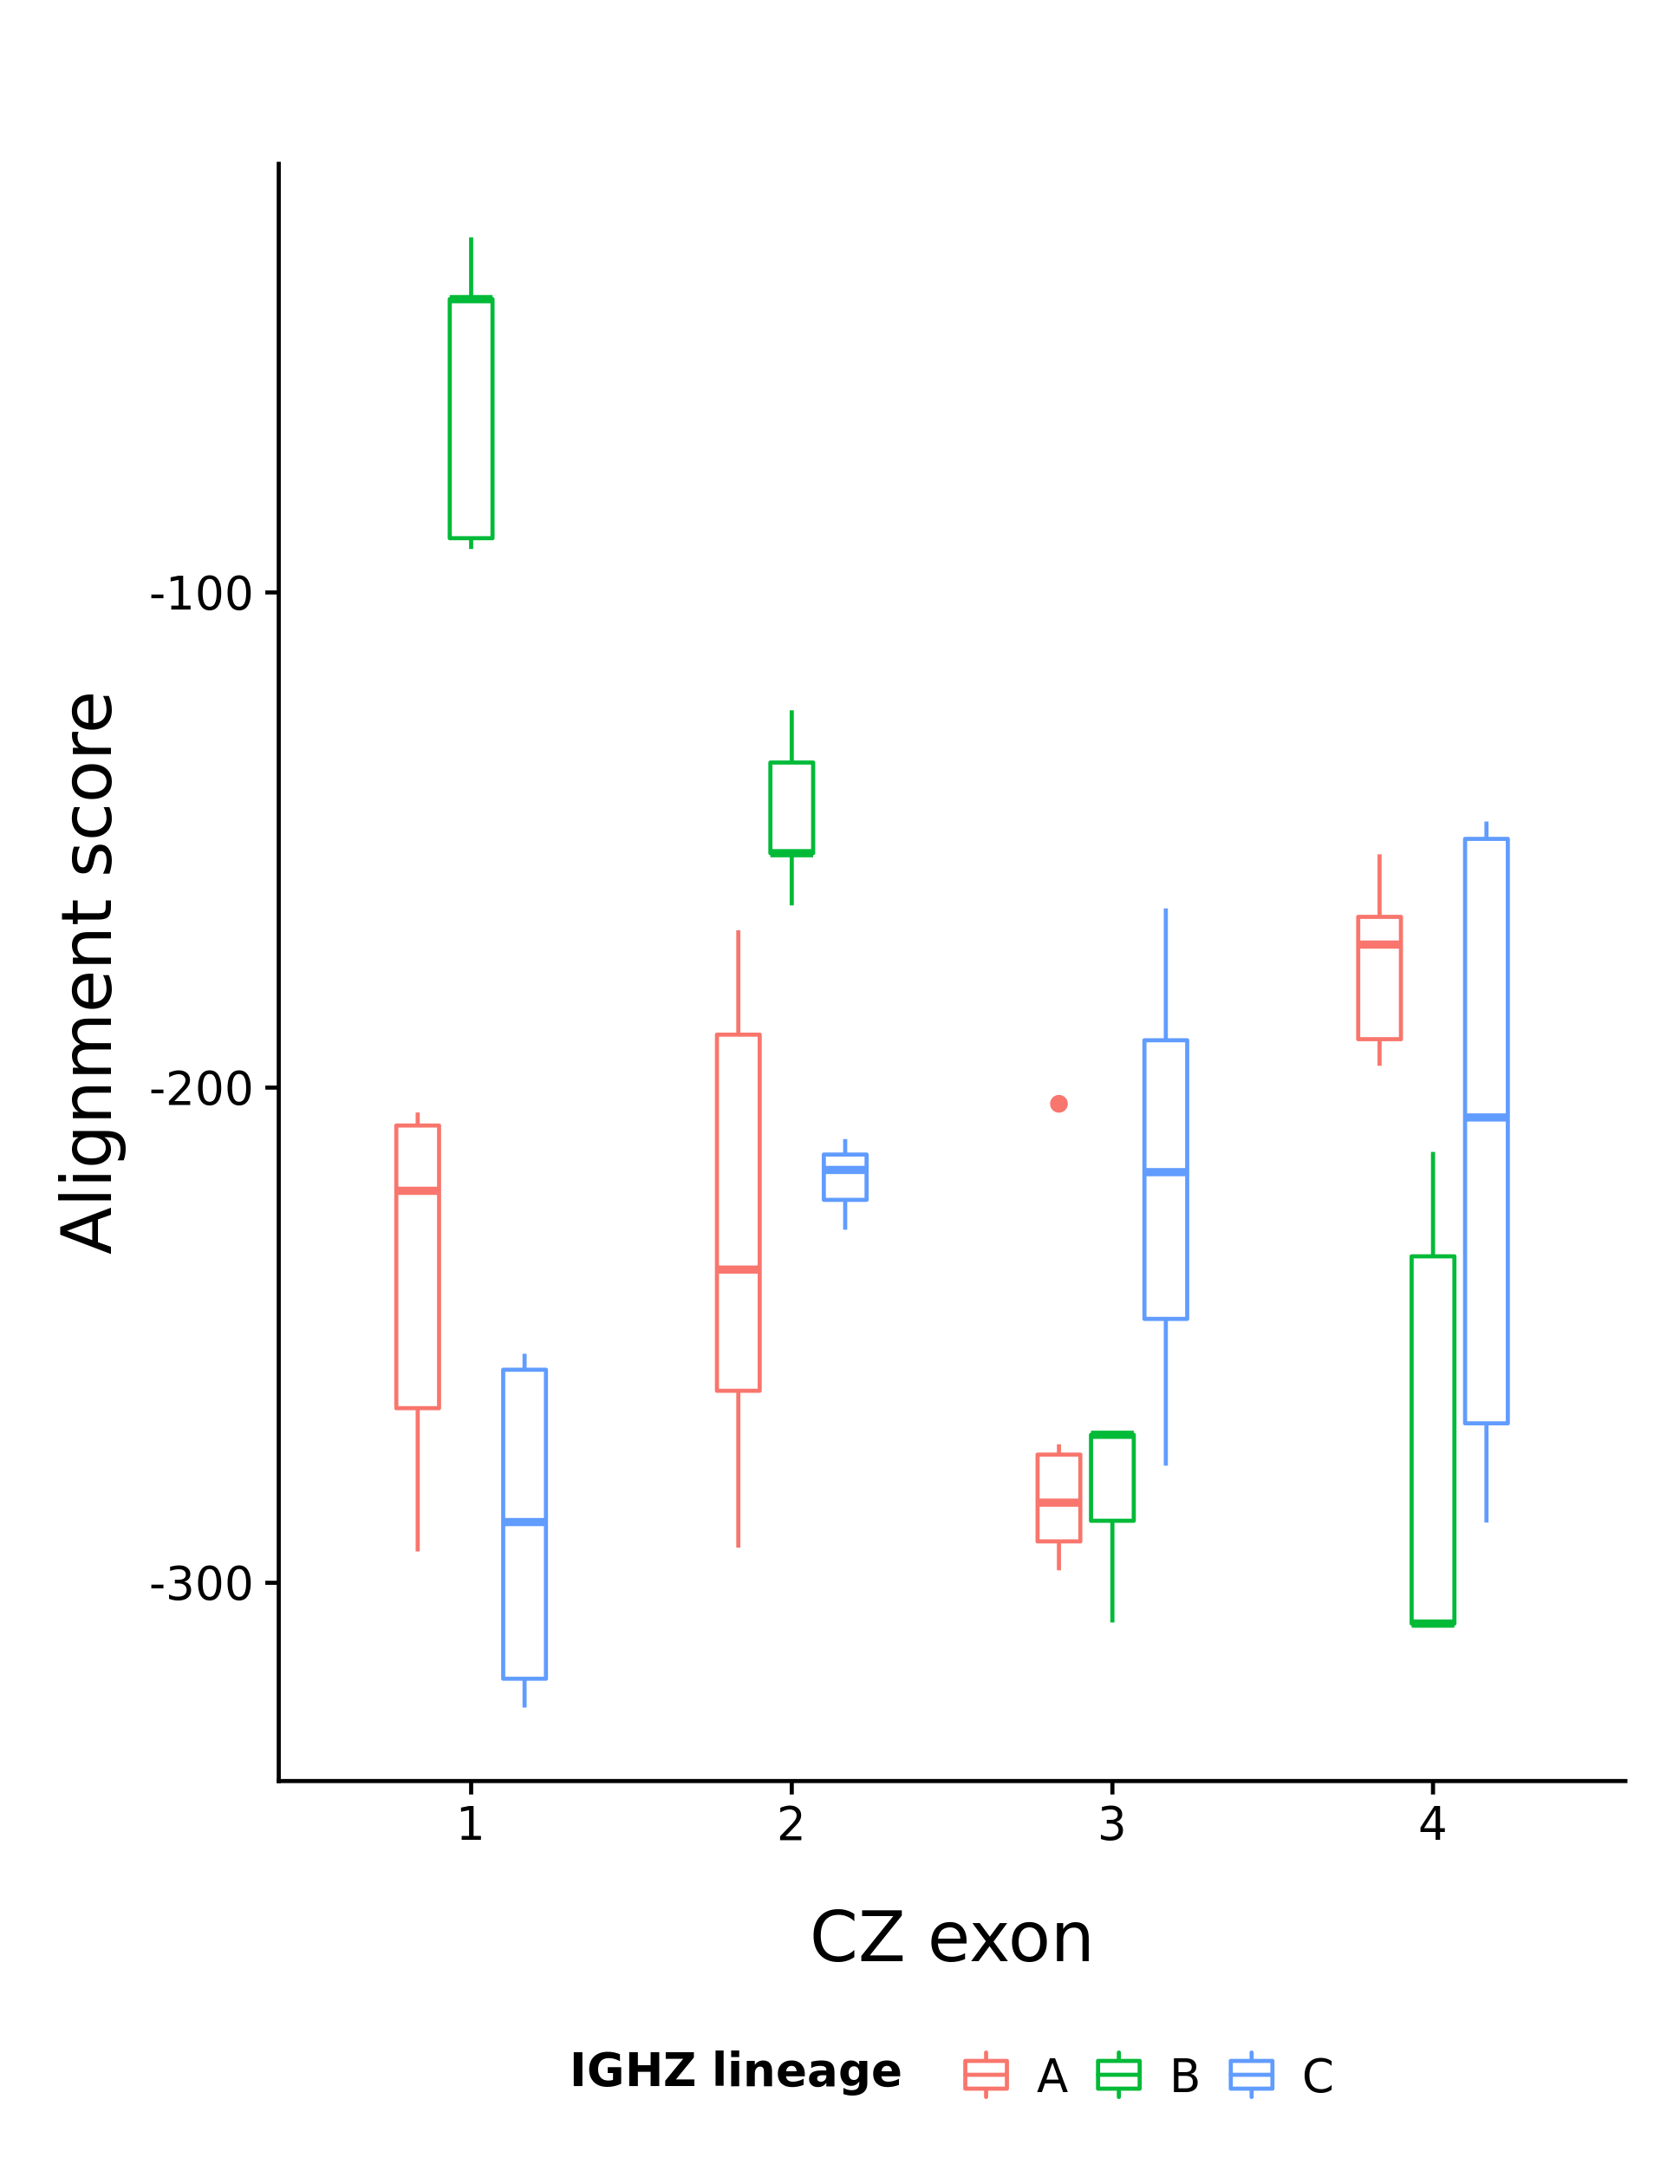
\includegraphics[width=0.8\textwidth]{_Figures/png/ppl-cz-aln-aa.png}
	\Caption{Subclass affinity of \igh{Z} in \species{Pachypanchax}{playfairii}}{Boxplots of Needleman-Wunsch alignment scores between the amino-acid sequences of \species{P.}{playfairii} \cz{} exons and those of seven other \igh{Z}-bearing cyprinodontiform species, demonstrating the differing affinity of different \species{P.}{playfairii} exons for each of the three \igh{Z} subclasses. Pairwise $p$-values were computed using nonparametric Mann-Whitney $U$ tests ($*: 0.01 < p \leq 0.05;~**: 0.001 < p \leq 0.01;~***: p \leq 0.001$).}
	\label{fig:ppl-cz-aln}
\end{figure}
	
In summary, in addition to the still-universal primitive antibody classes \igh{M} and \igh{D}, the cyprinodontiforms ancestrally possessed at least three variants of \igh{Z}, giving rise to multiple subclasses of \igh{Z} constant regions evolving in parallel across the clade. Each of these subclasses appears to have been lost in multiple cyprinodontiform species, with different species showing distinct patterns of retention and loss, and in at least one lineage -- that of \species{Pachypanchax}{playfairii} -- two different \igh{Z} lineages have fused to produce a chimeric isotype. All three subclasses are missing from a subset of species in the Nothobranchiidae (including \nfu), and also appear to have been independently lost in \species{Austrofundulus}{limnaeus}. Taken together, these data suggest a high degree of complexity and volatility in the evolution of mucosal adaptive immunity in the Cyprinodontiformes.

\newpage

\section{Discussion}

The teleost fishes are the largest and most diverse group of vertebrates, with nearly 30,000 species comprising almost half of extant vertebrate diversity \parencite{ravi2018divergent}. Of this vast variety of teleosts, only a few species, mostly those used extensively in aquaculture or scientific research, have undergone extensive study with regard to their immunoglobulin gene loci (\Cref{sec:intro_teleost_loci}). Studies in these model species have revealed a high level of structural diversity among teleost \igh{} loci, with huge variation in both size and organisation, as well as the existence of three distinct antibody isotypes in fish, of which two (\igh{M} and \igh{D}) are shared with tetrapods and one (\igh{Z}) appears to be teleost-specific. However, in many large and important teleost lineages, the genetic basis of B-cell-mediated humoral immunity remains unknown.

In this chapter, I presented two complete and ten partial assemblies of \igh{} loci from the Cyprinodontiformes, a diverse clade of primarily freshwater fishes for which no such loci have previously been characterised. The two complete assemblies were of the \igh{} loci of the turquoise killifish \nfu and the southern platyfish \xma, two important model species with an estimated divergence time of less than 80 Mya \parencite{hughes2018teleostphylo}. Despite their close relationship, these species show radically different locus organisations, with huge differences in VDJ number (24 \vh segments in \Nfu versus 125 in \Xma), locus organisation (two small subloci in opposite sense in \Nfu, one large unitary locus in \Xma) and isotype availability (no \igh{Z} in \Nfu, two distinct \igh{Z} regions in \Xma), as well as more subtle but still-important distinctions like differences in constant-region splicing behaviour (four exons in \Nfu \igh{M-TM}, five in \Xma). These results are consistent with previous findings of highly-diverse teleost loci and support a process of rapid evolution in the \igh{} locus. Characterisation of the constant regions of a further ten cyprinodontiform species confirmed this finding, with several groups of closely-related species (e.g. \nfu, \species{Nothobranchius}{orthonotus} and \species{Callopanchax}{toddi}) showing highly divergent locus structures and constant-region availability.

It is interesting to speculate on the origins of this extremely rapid diversification in gene structure. Very little is known about the relationship between environmental context and immune locus structure; it is possible that part of the variety in \igh{} gene locus structure in the Cyprinodontiformes represents divergent adaptations to different immune environments. Alternatively, this diversification may be primarily the result of unusually high rates of stochastic, non-adaptive changes in gene structure in germline \igh{}. Finally, at least some of the difference between locus structures in different species is likely to be attributable to differences in assembly quality; for example, the characterisation of medaka constant regions presented here contains many fewer unusual or incomplete constant regions than that presented in the published medaka \igh{} locus \parencite{magadan2011medaka}, primarily due to the increased quality of the more recent medaka genome assemblies.

Before the publication of this work, only two teleost species (medaka and channel catfish) were known or thought to lack the \igh{Z} antibody isotype from their \igh{} loci, out of more than ten species with published locus characterisations. This relative rarity of observed absence, combined with the apparent importance of \igh{Z} in teleost mucosal immunity, suggested that the loss of \igh{Z} was likely to be a rare and unusual event. However, in addition to confirming the absence of \igh{Z} in medaka, this study identified four new teleost species (\nfu, \species{Nothobranchius}{orthonotus}, \species{Aphyosemion}{australe} and \species{Austrofundulus}{limnaeus}) that appear to lack \igh{Z} constant regions in their \igh{} loci, representing two distinct and previously unknown loss events independent from that affecting the closely-related medaka. This finding, which triples the number of known teleost species without \igh{Z} and doubles the number of known loss events, is even more striking when combined with the discovery that the cyprinidontiform common ancestor likely had no fewer than three distinct \igh{Z} constant regions, all of which would have had to be lost on the way to any \igh{Z}-free lineage. The high level of observed variability in \igh{Z} prevalence among the cyprinidontiforms suggests that the presence/absence of \igh{Z} in the wider teleost clade may be much more volatile than suggested by previously available locus data, and raises the possibility that, given sufficiently high-density analysis of other teleost lineages, a similar frequency of \igh{Z}-lacking species may also be found elsewhere. However, it may also be the case that the apparently high frequency of \igh{Z} loss events in the Atherinomorpha is a special case, arising from chance, an unusual selective environment, or limitations in the available genome assemblies.

The absence of \igh{Z} from so many species in the Atherinomorpha naturally raises the important question of how the mucosal adaptive immune system in these species differs from that of their \igh{Z}-bearing relatives. Data from rainbow trout suggest that \igh{T} (an alternative name for \igh{Z} in some species) plays a specialised role in antibody immune responses at multiple mucosal surfaces, with increased prevalence of \igh{T}$^+$ B-cells and secreted IGHT antibodies relative to serum, a primarily \igh{T}-dependent response to mucosal infections, and a much higher rate of bacterial coating by IGHT in skin and gut flora relative to IGHM \parencite{zhang2010igtgut,xu2013igtskin}.
If these findings hold for other teleost species, it is not clear how \igh{Z}-lacking teleost species carry out specialised immune functions at mucosal barriers: how, and to what extent, can \igh{M} compensate for the loss of a specialised mucosal isotype? This question is especially interesting in the case of \igh{Z}-lacking species with close \igh{Z}-bearing relatives (e.g. \nfu and \species{Callopanchax}{toddi}, or perhaps \species{Austrofundulus}{limnaeus} and \species{Kryptolebias}{marmoratus}); if it is the case that mucosal immune responses differ systematically between these species, such that \igh{M} takes up some or all of the roles normally played by \igh{Z}, then uncovering the mechanisms by which this shift is regulated could reveal important new insights into decision-making and control of humoral adaptive immunity.

One important difference between the \Xma and \Nfu loci whose evolution is more difficult to investigate using genomic data is the exon usage behaviour of the different splice isoforms present in the transcriptome of each species. In \Xma, transmembrane \igh{M} adopts the same configuration as that seen in most teleosts for which this has been investigated: a five-exon isoform in which the end of \cm{3} is spliced to the start of TM1 and \cm{4} is excised. Conversely, in \Nfu \igh{M-TM} adopts the same four-exon configuration observed in medaka, in which \cm{3} is also excluded. Given that \Xma adopts the primitive configuration, the recurrence of the same unusual configuration in both medaka and turquoise killifish is surprising, and indicates that both configurations are present in the Cyprinodontiformes; however, without more information about the mechanisms and genomic sequence correlates underlying this difference, it is impossible to distinguish an independent origin of the derived phenotype in medaka and \Nfu from a reversion to the primitive phenotype in \Xma. It is also not clear at present what functional differences, if any, arise from this difference in exon usage, although it seems unlikely that the shorter four-exon form of \igh{M-TM} would persist in multiple species if it prevented effective antibody development, selection, or antigen response.

As a result of the research findings presented in this chapter, a number of previously-uncharacterised teleost species now have databases of constant regions available. As a result, primer design for targeted RNA-sequencing of expressed antibody sequences is now possible for these taxa, enabling quantitative immune-repertoire sequencing approaches in a large number of closely-related cyprinidontiform species. In addition to the special interest of immune-repertoire data from any one of these new species (e.g. \Nfu for immune-repertoire ageing or \Xma for ecological and evolutionary research), the possibility of sequencing the repertoires of several related species adds an exciting comparative dimension. This comparative element would be especially interesting in the context of investigating the repertoire responses of closely related species with different \igh{Z} genotypes. In combination with the genomic and functional comparisons discussed above, the novel possibility of large-scale comparative repertoire studies arising as a result of this research establishes the Cyprinidontiformes, and especially the African killifishes, as a highly-promising group of model species for comparative evolutionary immunology.

% TODO: Ask Dario re discussion
